%Einbindung Pakete
\documentclass[11pt,a4paper,oneside]{scrartcl}

%Pakete

%Style
\usepackage[left=2.5cm,right=2.5cm,top=2.0cm,bottom=2.5cm,footskip=1.5cm,head=25pt]{geometry}		
\usepackage{setspace}
\usepackage[bottom,hang]{footmisc}
\usepackage{longtable}

%Sprache
\usepackage[T1]{fontenc}  
\usepackage[utf8]{inputenc}
\usepackage[english]{babel}
\usepackage{eurosym}
\usepackage{lmodern}
\usepackage{lipsum}
\usepackage{csquotes}

%Mathe- Umgebung
\usepackage{amsmath}
\usepackage{amssymb}
\usepackage{amsfonts}

%Grafiken
\usepackage{graphicx}																								
\usepackage{psfrag}
\usepackage{wrapfig}
\usepackage{subfigure}
\usepackage[headsepline,automark]{scrlayer-scrpage}

%Tabellenstil
\usepackage{tabularx}
\usepackage{multirow}
\usepackage{booktabs}
\usepackage{colortbl}

%Referenzen
\usepackage[backend=biber, style=numeric, sorting=nty]{biblatex}
\addbibresource{Quellen.bib}  

%Das hyperref paket führt zu Problemen mit der Internet-Link Darstellung, da bei diesen mit aktivem Paket kein Zeilenumbruch möglich ist ggf. kann hier eine eigene Lösung gefunden werden
\usepackage[hidelinks]{hyperref}

%Grafikpafad
\graphicspath{{./Abbildungen/}}

%Zusätzliche Pakete
\usepackage{caption}
\usepackage{units}
\usepackage{float}
\usepackage[]{xcolor}
\usepackage{colortbl}
\usepackage{hhline}
\usepackage{pdfpages}

%Nachträglich hinzugefügte Pakete
%\usepackage{auto-pst-pdf}


%For header
\clearpairofpagestyles

\ihead{\responsibleName}
\chead{\headmark}
\cfoot{\pagemark}

\newcommand{\responsibleName}{}
\newcommand{\setresponsible}[1]{\renewcommand{\responsibleName}{#1}}

%Initialisierung des Dokuments
\begin{document}

%Einbindung unterschiedlicher Befehlsänderungen
\input{style}

\parindent 0cm

%Zeilenabstand	
\onehalfspacing			 									
\addtolength{\footskip}{-8mm}

%Titelseite
\begin{titlepage}
    \begin{center}
        
\includegraphics[width=0.25\textwidth]{HTWLogo}\\

        \vspace*{\fill}

        \rule{\textwidth}{0.4pt}\\[0.8em]
        \textcolor{HTWGreen}{\Large\textbf{Production, Characterization, and Utilization of Biochar from Slaughterhouse Digestates via Pyrolysis and $H_2O$-Activation}}\\[0.8em]
        \rule{\textwidth}{0.4pt}

        \vspace*{\fill}

                \LARGE Masterarbeit

        \vspace*{\fill}

        \Large Regenerative Energien (M)

        \bigskip
        \textcolor{HTWGreen}{\Large\textbf{Fachbereich 1: Ingenieurwissenschaften - Energie und Information}}

        \bigskip
        \Large Hochschule für Technik und Wirtschaft Berlin

        \vspace*{\fill}

        vorgelegt von

        \vspace*{0.5em}

        \begin{table}[H]
            \centering
            \large
            \begin{tabular}{|l|c|}
                \hline
                \rowcolor[cmyk]{0.55, 0.00, 1.00, 0.00} \textbf{Name} & \textbf{Matrikelnummer} \\
                \hline
                Regen Wijaya & 575946\\
                \hline
                Surya Salim & 576214\\
                \hline
            \end{tabular}
        \end{table}

        \vspace*{\fill}

        Datum:\\
        Berlin, 14.09.2026

        \vspace*{\fill}

        \Large Erstgutachter\_in: Prof. Dr.-Ing. Mirko Barz\\
        \Large Zweitgutachter\_in: Dipl.-Ing. Guy Kabengele

        \vspace*{\fill}
    \end{center}
\end{titlepage}
\newpage

%Abstract (dieser ist für Laborprotokolle in der Regel nicht notwendig)
\begin{abstract}

\begin{center}
\normalsize \textbf{Abstract}\\
\end{center}

\noindent
Slaughterhouse digestate is a residue that normally carries a disposal cost. The aim of this work is to examines whether it can be pyrolysed into biochar, upgraded by steam activation into a sulfur sorbent, and also how the steam route compares with the CO$_2$ activation used in a preceding project work. Biochar was produced from French (and also Algerian) slaughterhouse digestate at 400, 500, and 600\,$^{\circ}$C. These chars are then characterized by bomb calorimetry, CHNS elemental analysis, and N$_2$ adsorption. The French chars were then steam-activated at 700\,$^{\circ}$C and loaded with sulfur from H$_2$S. The French digestate gave the higher solid yield at every temperature, falling from 45.7 to 42.2\,\% against 37.4 to 33.5\,\% for the Algerian material. Ash rose from 22.6\,\% in the digestate to 43.5--50.0\,\% in the chars and held the gross calorific value at 14.1--14.2\,MJ\,kg$^{-1}$, against 25.1--28.2\,MJ\,kg$^{-1}$ on an ash-free basis, so the low heating value reflects mineral dilution rather than incomplete pyrolysis. Ash-free carbon rose from 67.2 to 76.0\,\% and the atomic H/C ratio fell from 0.481 to 0.163. Steam activation at 0.5\,mL\,g$^{-1}$ removed 11--18\,\% of the char mass, the loss falling as the precursor pyrolysis temperature rose. The specific surface area increased from 0.8--32\,m$^2$\,g$^{-1}$ in the pristine chars to 89--146\,m$^2$\,g$^{-1}$ after activation and sulfur loading, with the maximum at the 500\,$^{\circ}$C precursor rather than at the most carbonized char. Every sample took up sulfur, 36--64\,mg\,g$^{-1}$ by weighing and 5.2--6.8\,\% S by CHNS against about 1.5\,\% in the pristine chars, which is two to three times the uptake of the CO$_2$-activated chars of the preceding work, although the feedstocks differed and no surface-area data exist for the CO$_2$ samples. No single pyrolysis temperature suited every purpose: 500\,$^{\circ}$C gave the most developed pore structure for adsorption, 400\,$^{\circ}$C the highest nitrogen content for soil application, and 600\,$^{\circ}$C the lowest H/C ratio for carbon storage, while the ash content rules all three out as a solid fuel. At 146\,m$^2$\,g$^{-1}$ the char stays well below commercial activated carbon, so the realistic case is a low-cost sorbent for removing H$_2$S from the biogas of the same digestion.
\noindent

\end{abstract}


\vspace{0.5em}

\noindent

\vspace{0.8em}
\newpage

%
 
\begin{center}
\normalsize \textbf{Acknowledgements}\\
\end{center}

    \noindent

We would like to convey our sincerest appreciation and gratitude to the following individuals who helped us greatly in completing this thesis. First and foremost, we would also like to express our sincerest gratitude to Prof. Dr.-Ing Mirko Barz, who offered us the topic of production, characterization, and utilization of biochar from slaughterhouse digestates via pyrolysis and $H_2$O-activation, and whose course ultimately drove us to choose this topic. His insightful suggestions and guidance helped shape this work.

\vspace{0.3em}

We would like to acknowledge our second expert opinion, Dipl.-Ing. Guy-Rod Kabengele, for giving us insight throughout the thesis. His feedback on our methodology and the interpretation of our results helped us improve the work at several stages, and his suggestions pointed us toward clearer and more precise explanations. We appreciate the time he took to discuss our progress with us and would like to thank him. 

\vspace{0.3em}

We would also like to acknowledge Mr. Martin Krüger for helping us produce the biochar and for determining its calorific value, Mr. Steffen Kadow for assisting us in activating the biochar, and Mr. Adrian Lengemann for his support during the sulfur-loading process. Without their support, this work would not have advanced so successfully. Therefore, we would like to thank them with our deepest gratitude. 

\vspace{0.3em}

Last but not least, we would like to express how grateful we are to our family and friends for their unwavering love and support. We are especially thankful to our parents, who gave us the opportunity to experience this journey and supported us all the way to the end.

%\newpage

\pagenumbering{roman}

%Inhaltsverzeichnis
\setcounter{tocdepth}{3}
\tableofcontents
\newpage

%Abbildungsverzeichnis und Tabellenverzeichnis
\listoffigures
\listoftables
\newpage

%Symbol- und Abkürzungsverzeichnis
%%=====================================================================
%  List of Symbols and Abbreviations
%  Include in the main file with %=====================================================================
%  List of Symbols and Abbreviations
%  Include in the main file with %=====================================================================
%  List of Symbols and Abbreviations
%  Include in the main file with \input{Symbolverzeichnis}
%  (place it after \listoftables, before \pagenumbering{arabic})
%=====================================================================

\addtocounter{table}{-1}
\bigskip
\Large \textsf{\textbf{List of Symbols}}
\normalsize
\vspace{0.5em}

%---------------------------------------------------------------------
%  LATIN SYMBOLS
%---------------------------------------------------------------------
\begin{longtable}{p{3cm}p{9.5cm}p{2.5cm}}
\textbf{Symbol} & \textbf{Meaning} & \textbf{Unit}\\
\hline
\endfirsthead
\textbf{Symbol} & \textbf{Meaning} & \textbf{Unit}\\
\hline
\endhead
\multicolumn{3}{l}{\textit{Latin symbols}}\\[0.3em]
\(A\)                        & Specific surface area                                           & m$^2$\,g$^{-1}$\\
\(A_m\)                      & Cross-sectional area of one adsorbate molecule                  & m$^2$\\
\(C\)                        & BET constant                                                    & --\\
\(EDF\)                      & Energy densification factor                                     & --\\
\(H_0\)                      & Higher heating value (Brennwert, GCV)                           & MJ\,kg$^{-1}$\\
\(H_u\)                      & Lower heating value (Heizwert, NCV)                             & MJ\,kg$^{-1}$\\
\(H_d\)                      & Hydrogen content on a dry basis                                 & wt\,\%\\
\(HHV_d\)                    & Gross calorific value on a dry basis                            & MJ\,kg$^{-1}$\\
\(LHV_{p,ar}\)               & Lower heating value, constant pressure, as received             & MJ\,kg$^{-1}$\\
\(M\)                        & Moisture content, as received                                   & wt\,\%\\
\(M_0\)                      & Biochar mass before H$_2$O activation                           & g\\
\(M_1\)                      & Biochar mass after H$_2$O activation                            & g\\
\(M_{\mathrm{H_2}}\)         & Molar mass of hydrogen (2.016)                                  & g\,mol$^{-1}$\\
\(M_{\mathrm{H_2O}}\)        & Molar mass of water (18.015)                                    & g\,mol$^{-1}$\\
\(m\)                        & Sample mass burned in the calorimeter                           & g\\
\(m_0\)                      & Sample mass used for ash determination                          & g\\
\(m_{\mathrm{ash}}\)         & Residual ash mass                                               & g\\
\(m_{biochar}\)              & Mass of biochar (energy-yield relation)                         & g\\
\(m_{feedstock}\)            & Mass of feedstock (energy-yield relation)                       & g\\
\(m_{Biochar}\)              & Mass of biochar recovered after pyrolysis                       & g\\
\(m_{Digestate}\)            & Mass of digestate charged to the reactor                        & g\\
\(m_{before}\)               & Biochar mass before H$_2$O activation                           & g\\
\(m_{after,wet}\)            & Biochar mass after activation, before drying                    & g\\
\(m_{after,dry}\)            & Biochar mass after activation, after drying                     & g\\
\(m_{\mathrm{before,s}}\)    & Biochar mass before sulfur loading                              & g\\
\(m_{\mathrm{after,s}}\)     & Biochar mass after sulfur loading                               & g\\
\(m_{Nutrings}\)             & Combined mass of the two inert metal rings (20.74)              & g\\
\(m_p\)                      & Sample mass used in the BET measurement                         & g\\
\(N_A\)                      & Avogadro constant                                               & mol$^{-1}$\\
\(O\)                        & Oxygen content, calculated by difference                         & wt\,\%\\
\(O_{\mathrm{spez.}}\)       & Specific surface area determined by the BET method              & m$^2$\,g$^{-1}$\\
\(p\)                        & Equilibrium pressure of the adsorptive                           & Pa\\
\(p_0\)                      & Saturation vapour pressure of the adsorptive                     & Pa\\
\(p/p_0\)                    & Relative pressure                                               & --\\
\(Q_{\mathrm{ext}}\)         & Sum of external corrections in bomb calorimetry                 & J\\
\(Q_{\mathrm{S}}\)           & Sulfur loading capacity derived from CHNS analysis              & mg\,g$^{-1}$\\
\(q_s\)                      & Sulfur loading capacity determined gravimetrically              & mg\,g$^{-1}$\\
\(q_{V,gr}\)                 & Gross calorific value at constant volume                        & J\,g$^{-1}$\\
\(T\)                        & Temperature                                                     & $^\circ$C\\
\(T_{\mathrm{pyr}}\)         & Pyrolysis temperature                                           & $^\circ$C\\
\(V\)                        & Gas volume adsorbed at equilibrium pressure $p$                 & cm$^3$\\
\(V_{\mathrm{Mono}}\)        & Gas volume adsorbed in a complete monolayer                     & cm$^3$\\
\(V_m\)                      & Molar volume of the adsorptive at STP                           & cm$^3$\,mol$^{-1}$\\
\(V_p\)                      & Total pore volume                                               & cm$^3$\,g$^{-1}$\\
\(w_{bio}\)                  & True moisture content of the biochar                            & wt\,\%\\
\(w_{dryer}\)                & Moisture content reported by the halogen moisture analyser      & wt\,\%\\
\(w_{\mathrm{S,base}}\)      & Sulfur mass fraction of the pristine biochar                    & wt\,\%\\
\(w_{\mathrm{S,loaded}}\)    & Sulfur mass fraction after sulfur loading                        & wt\,\%\\
\(Y\)                        & Biochar (mass) yield                                            & \%\\
\(Y_E\)                      & Energy yield                                                    & \%\\
\\[0.3em]
\multicolumn{3}{l}{\textit{Greek symbols}}\\[0.3em]
\(\Delta m_{active,wet}\)    & Activation mass loss on a wet basis                             & \%\\
\(\Delta m_{loss}\)          & Total mass loss (activation and residual moisture)              & \%\\
\(\Delta T\)                 & Corrected temperature rise in the calorimeter                    & K\\
\(\varepsilon\)              & Effective heat capacity of the calorimeter system                & J\,K$^{-1}$\\
\\[0.3em]
\multicolumn{3}{l}{\textit{Subscripts}}\\[0.3em]
\(ar\)                       & As received                                                     & --\\
\(d\)                        & Dry basis                                                       & --\\
\(f\)                        & Free active carbon site (e.g.\ C$_f$)                           & --\\
\(gr\)                       & Gross                                                           & --\\
\(p\)                        & At constant pressure                                            & --\\
\(s\)                        & Sulfur loading step                                             & --\\
\(V\)                        & At constant volume                                              & --\\
\end{longtable}

\newpage

%---------------------------------------------------------------------
%  ABBREVIATIONS
%---------------------------------------------------------------------
\addtocounter{table}{-1}
\bigskip
\Large \textsf{\textbf{List of Abbreviations}}
\normalsize
\vspace{0.5em}

\begin{longtable}{p{3cm}p{12cm}}
\textbf{Abbreviation} & \textbf{Meaning}\\
\hline
\endfirsthead
\textbf{Abbreviation} & \textbf{Meaning}\\
\hline
\endhead
AAEM   & Alkali and alkaline earth metals\\
AC     & Ash content\\
BC     & Biochar\\
BET    & Brunauer--Emmett--Teller (method for specific surface area)\\
CHNS   & Carbon, hydrogen, nitrogen and sulfur elemental analysis\\
EBC    & European Biochar Certificate\\
EDF    & Energy densification factor\\
EDX    & Energy-dispersive X-ray spectroscopy\\
FC     & Fixed carbon\\
GCV    & Gross calorific value\\
HHV    & Higher heating value\\
IUPAC  & International Union of Pure and Applied Chemistry\\
LHV    & Lower heating value\\
LOD    & Loss on drying\\
NCV    & Net calorific value\\
OFMSW  & Organic fraction of municipal solid waste\\
PY     & Pyrolysis yield\\
SD     & Standard deviation\\
SEM    & Scanning electron microscopy\\
SSA    & Specific surface area\\
STP    & Standard temperature and pressure\\
VM     & Volatile matter\\
\end{longtable}

%  (place it after \listoftables, before \pagenumbering{arabic})
%=====================================================================

\addtocounter{table}{-1}
\bigskip
\Large \textsf{\textbf{List of Symbols}}
\normalsize
\vspace{0.5em}

%---------------------------------------------------------------------
%  LATIN SYMBOLS
%---------------------------------------------------------------------
\begin{longtable}{p{3cm}p{9.5cm}p{2.5cm}}
\textbf{Symbol} & \textbf{Meaning} & \textbf{Unit}\\
\hline
\endfirsthead
\textbf{Symbol} & \textbf{Meaning} & \textbf{Unit}\\
\hline
\endhead
\multicolumn{3}{l}{\textit{Latin symbols}}\\[0.3em]
\(A\)                        & Specific surface area                                           & m$^2$\,g$^{-1}$\\
\(A_m\)                      & Cross-sectional area of one adsorbate molecule                  & m$^2$\\
\(C\)                        & BET constant                                                    & --\\
\(EDF\)                      & Energy densification factor                                     & --\\
\(H_0\)                      & Higher heating value (Brennwert, GCV)                           & MJ\,kg$^{-1}$\\
\(H_u\)                      & Lower heating value (Heizwert, NCV)                             & MJ\,kg$^{-1}$\\
\(H_d\)                      & Hydrogen content on a dry basis                                 & wt\,\%\\
\(HHV_d\)                    & Gross calorific value on a dry basis                            & MJ\,kg$^{-1}$\\
\(LHV_{p,ar}\)               & Lower heating value, constant pressure, as received             & MJ\,kg$^{-1}$\\
\(M\)                        & Moisture content, as received                                   & wt\,\%\\
\(M_0\)                      & Biochar mass before H$_2$O activation                           & g\\
\(M_1\)                      & Biochar mass after H$_2$O activation                            & g\\
\(M_{\mathrm{H_2}}\)         & Molar mass of hydrogen (2.016)                                  & g\,mol$^{-1}$\\
\(M_{\mathrm{H_2O}}\)        & Molar mass of water (18.015)                                    & g\,mol$^{-1}$\\
\(m\)                        & Sample mass burned in the calorimeter                           & g\\
\(m_0\)                      & Sample mass used for ash determination                          & g\\
\(m_{\mathrm{ash}}\)         & Residual ash mass                                               & g\\
\(m_{biochar}\)              & Mass of biochar (energy-yield relation)                         & g\\
\(m_{feedstock}\)            & Mass of feedstock (energy-yield relation)                       & g\\
\(m_{Biochar}\)              & Mass of biochar recovered after pyrolysis                       & g\\
\(m_{Digestate}\)            & Mass of digestate charged to the reactor                        & g\\
\(m_{before}\)               & Biochar mass before H$_2$O activation                           & g\\
\(m_{after,wet}\)            & Biochar mass after activation, before drying                    & g\\
\(m_{after,dry}\)            & Biochar mass after activation, after drying                     & g\\
\(m_{\mathrm{before,s}}\)    & Biochar mass before sulfur loading                              & g\\
\(m_{\mathrm{after,s}}\)     & Biochar mass after sulfur loading                               & g\\
\(m_{Nutrings}\)             & Combined mass of the two inert metal rings (20.74)              & g\\
\(m_p\)                      & Sample mass used in the BET measurement                         & g\\
\(N_A\)                      & Avogadro constant                                               & mol$^{-1}$\\
\(O\)                        & Oxygen content, calculated by difference                         & wt\,\%\\
\(O_{\mathrm{spez.}}\)       & Specific surface area determined by the BET method              & m$^2$\,g$^{-1}$\\
\(p\)                        & Equilibrium pressure of the adsorptive                           & Pa\\
\(p_0\)                      & Saturation vapour pressure of the adsorptive                     & Pa\\
\(p/p_0\)                    & Relative pressure                                               & --\\
\(Q_{\mathrm{ext}}\)         & Sum of external corrections in bomb calorimetry                 & J\\
\(Q_{\mathrm{S}}\)           & Sulfur loading capacity derived from CHNS analysis              & mg\,g$^{-1}$\\
\(q_s\)                      & Sulfur loading capacity determined gravimetrically              & mg\,g$^{-1}$\\
\(q_{V,gr}\)                 & Gross calorific value at constant volume                        & J\,g$^{-1}$\\
\(T\)                        & Temperature                                                     & $^\circ$C\\
\(T_{\mathrm{pyr}}\)         & Pyrolysis temperature                                           & $^\circ$C\\
\(V\)                        & Gas volume adsorbed at equilibrium pressure $p$                 & cm$^3$\\
\(V_{\mathrm{Mono}}\)        & Gas volume adsorbed in a complete monolayer                     & cm$^3$\\
\(V_m\)                      & Molar volume of the adsorptive at STP                           & cm$^3$\,mol$^{-1}$\\
\(V_p\)                      & Total pore volume                                               & cm$^3$\,g$^{-1}$\\
\(w_{bio}\)                  & True moisture content of the biochar                            & wt\,\%\\
\(w_{dryer}\)                & Moisture content reported by the halogen moisture analyser      & wt\,\%\\
\(w_{\mathrm{S,base}}\)      & Sulfur mass fraction of the pristine biochar                    & wt\,\%\\
\(w_{\mathrm{S,loaded}}\)    & Sulfur mass fraction after sulfur loading                        & wt\,\%\\
\(Y\)                        & Biochar (mass) yield                                            & \%\\
\(Y_E\)                      & Energy yield                                                    & \%\\
\\[0.3em]
\multicolumn{3}{l}{\textit{Greek symbols}}\\[0.3em]
\(\Delta m_{active,wet}\)    & Activation mass loss on a wet basis                             & \%\\
\(\Delta m_{loss}\)          & Total mass loss (activation and residual moisture)              & \%\\
\(\Delta T\)                 & Corrected temperature rise in the calorimeter                    & K\\
\(\varepsilon\)              & Effective heat capacity of the calorimeter system                & J\,K$^{-1}$\\
\\[0.3em]
\multicolumn{3}{l}{\textit{Subscripts}}\\[0.3em]
\(ar\)                       & As received                                                     & --\\
\(d\)                        & Dry basis                                                       & --\\
\(f\)                        & Free active carbon site (e.g.\ C$_f$)                           & --\\
\(gr\)                       & Gross                                                           & --\\
\(p\)                        & At constant pressure                                            & --\\
\(s\)                        & Sulfur loading step                                             & --\\
\(V\)                        & At constant volume                                              & --\\
\end{longtable}

\newpage

%---------------------------------------------------------------------
%  ABBREVIATIONS
%---------------------------------------------------------------------
\addtocounter{table}{-1}
\bigskip
\Large \textsf{\textbf{List of Abbreviations}}
\normalsize
\vspace{0.5em}

\begin{longtable}{p{3cm}p{12cm}}
\textbf{Abbreviation} & \textbf{Meaning}\\
\hline
\endfirsthead
\textbf{Abbreviation} & \textbf{Meaning}\\
\hline
\endhead
AAEM   & Alkali and alkaline earth metals\\
AC     & Ash content\\
BC     & Biochar\\
BET    & Brunauer--Emmett--Teller (method for specific surface area)\\
CHNS   & Carbon, hydrogen, nitrogen and sulfur elemental analysis\\
EBC    & European Biochar Certificate\\
EDF    & Energy densification factor\\
EDX    & Energy-dispersive X-ray spectroscopy\\
FC     & Fixed carbon\\
GCV    & Gross calorific value\\
HHV    & Higher heating value\\
IUPAC  & International Union of Pure and Applied Chemistry\\
LHV    & Lower heating value\\
LOD    & Loss on drying\\
NCV    & Net calorific value\\
OFMSW  & Organic fraction of municipal solid waste\\
PY     & Pyrolysis yield\\
SD     & Standard deviation\\
SEM    & Scanning electron microscopy\\
SSA    & Specific surface area\\
STP    & Standard temperature and pressure\\
VM     & Volatile matter\\
\end{longtable}

%  (place it after \listoftables, before \pagenumbering{arabic})
%=====================================================================

\addtocounter{table}{-1}
\bigskip
\Large \textsf{\textbf{List of Symbols}}
\normalsize
\vspace{0.5em}

%---------------------------------------------------------------------
%  LATIN SYMBOLS
%---------------------------------------------------------------------
\begin{longtable}{p{3cm}p{9.5cm}p{2.5cm}}
\textbf{Symbol} & \textbf{Meaning} & \textbf{Unit}\\
\hline
\endfirsthead
\textbf{Symbol} & \textbf{Meaning} & \textbf{Unit}\\
\hline
\endhead
\multicolumn{3}{l}{\textit{Latin symbols}}\\[0.3em]
\(A\)                        & Specific surface area                                           & m$^2$\,g$^{-1}$\\
\(A_m\)                      & Cross-sectional area of one adsorbate molecule                  & m$^2$\\
\(C\)                        & BET constant                                                    & --\\
\(EDF\)                      & Energy densification factor                                     & --\\
\(H_0\)                      & Higher heating value (Brennwert, GCV)                           & MJ\,kg$^{-1}$\\
\(H_u\)                      & Lower heating value (Heizwert, NCV)                             & MJ\,kg$^{-1}$\\
\(H_d\)                      & Hydrogen content on a dry basis                                 & wt\,\%\\
\(HHV_d\)                    & Gross calorific value on a dry basis                            & MJ\,kg$^{-1}$\\
\(LHV_{p,ar}\)               & Lower heating value, constant pressure, as received             & MJ\,kg$^{-1}$\\
\(M\)                        & Moisture content, as received                                   & wt\,\%\\
\(M_0\)                      & Biochar mass before H$_2$O activation                           & g\\
\(M_1\)                      & Biochar mass after H$_2$O activation                            & g\\
\(M_{\mathrm{H_2}}\)         & Molar mass of hydrogen (2.016)                                  & g\,mol$^{-1}$\\
\(M_{\mathrm{H_2O}}\)        & Molar mass of water (18.015)                                    & g\,mol$^{-1}$\\
\(m\)                        & Sample mass burned in the calorimeter                           & g\\
\(m_0\)                      & Sample mass used for ash determination                          & g\\
\(m_{\mathrm{ash}}\)         & Residual ash mass                                               & g\\
\(m_{biochar}\)              & Mass of biochar (energy-yield relation)                         & g\\
\(m_{feedstock}\)            & Mass of feedstock (energy-yield relation)                       & g\\
\(m_{Biochar}\)              & Mass of biochar recovered after pyrolysis                       & g\\
\(m_{Digestate}\)            & Mass of digestate charged to the reactor                        & g\\
\(m_{before}\)               & Biochar mass before H$_2$O activation                           & g\\
\(m_{after,wet}\)            & Biochar mass after activation, before drying                    & g\\
\(m_{after,dry}\)            & Biochar mass after activation, after drying                     & g\\
\(m_{\mathrm{before,s}}\)    & Biochar mass before sulfur loading                              & g\\
\(m_{\mathrm{after,s}}\)     & Biochar mass after sulfur loading                               & g\\
\(m_{Nutrings}\)             & Combined mass of the two inert metal rings (20.74)              & g\\
\(m_p\)                      & Sample mass used in the BET measurement                         & g\\
\(N_A\)                      & Avogadro constant                                               & mol$^{-1}$\\
\(O\)                        & Oxygen content, calculated by difference                         & wt\,\%\\
\(O_{\mathrm{spez.}}\)       & Specific surface area determined by the BET method              & m$^2$\,g$^{-1}$\\
\(p\)                        & Equilibrium pressure of the adsorptive                           & Pa\\
\(p_0\)                      & Saturation vapour pressure of the adsorptive                     & Pa\\
\(p/p_0\)                    & Relative pressure                                               & --\\
\(Q_{\mathrm{ext}}\)         & Sum of external corrections in bomb calorimetry                 & J\\
\(Q_{\mathrm{S}}\)           & Sulfur loading capacity derived from CHNS analysis              & mg\,g$^{-1}$\\
\(q_s\)                      & Sulfur loading capacity determined gravimetrically              & mg\,g$^{-1}$\\
\(q_{V,gr}\)                 & Gross calorific value at constant volume                        & J\,g$^{-1}$\\
\(T\)                        & Temperature                                                     & $^\circ$C\\
\(T_{\mathrm{pyr}}\)         & Pyrolysis temperature                                           & $^\circ$C\\
\(V\)                        & Gas volume adsorbed at equilibrium pressure $p$                 & cm$^3$\\
\(V_{\mathrm{Mono}}\)        & Gas volume adsorbed in a complete monolayer                     & cm$^3$\\
\(V_m\)                      & Molar volume of the adsorptive at STP                           & cm$^3$\,mol$^{-1}$\\
\(V_p\)                      & Total pore volume                                               & cm$^3$\,g$^{-1}$\\
\(w_{bio}\)                  & True moisture content of the biochar                            & wt\,\%\\
\(w_{dryer}\)                & Moisture content reported by the halogen moisture analyser      & wt\,\%\\
\(w_{\mathrm{S,base}}\)      & Sulfur mass fraction of the pristine biochar                    & wt\,\%\\
\(w_{\mathrm{S,loaded}}\)    & Sulfur mass fraction after sulfur loading                        & wt\,\%\\
\(Y\)                        & Biochar (mass) yield                                            & \%\\
\(Y_E\)                      & Energy yield                                                    & \%\\
\\[0.3em]
\multicolumn{3}{l}{\textit{Greek symbols}}\\[0.3em]
\(\Delta m_{active,wet}\)    & Activation mass loss on a wet basis                             & \%\\
\(\Delta m_{loss}\)          & Total mass loss (activation and residual moisture)              & \%\\
\(\Delta T\)                 & Corrected temperature rise in the calorimeter                    & K\\
\(\varepsilon\)              & Effective heat capacity of the calorimeter system                & J\,K$^{-1}$\\
\\[0.3em]
\multicolumn{3}{l}{\textit{Subscripts}}\\[0.3em]
\(ar\)                       & As received                                                     & --\\
\(d\)                        & Dry basis                                                       & --\\
\(f\)                        & Free active carbon site (e.g.\ C$_f$)                           & --\\
\(gr\)                       & Gross                                                           & --\\
\(p\)                        & At constant pressure                                            & --\\
\(s\)                        & Sulfur loading step                                             & --\\
\(V\)                        & At constant volume                                              & --\\
\end{longtable}

\newpage

%---------------------------------------------------------------------
%  ABBREVIATIONS
%---------------------------------------------------------------------
\addtocounter{table}{-1}
\bigskip
\Large \textsf{\textbf{List of Abbreviations}}
\normalsize
\vspace{0.5em}

\begin{longtable}{p{3cm}p{12cm}}
\textbf{Abbreviation} & \textbf{Meaning}\\
\hline
\endfirsthead
\textbf{Abbreviation} & \textbf{Meaning}\\
\hline
\endhead
AAEM   & Alkali and alkaline earth metals\\
AC     & Ash content\\
BC     & Biochar\\
BET    & Brunauer--Emmett--Teller (method for specific surface area)\\
CHNS   & Carbon, hydrogen, nitrogen and sulfur elemental analysis\\
EBC    & European Biochar Certificate\\
EDF    & Energy densification factor\\
EDX    & Energy-dispersive X-ray spectroscopy\\
FC     & Fixed carbon\\
GCV    & Gross calorific value\\
HHV    & Higher heating value\\
IUPAC  & International Union of Pure and Applied Chemistry\\
LHV    & Lower heating value\\
LOD    & Loss on drying\\
NCV    & Net calorific value\\
OFMSW  & Organic fraction of municipal solid waste\\
PY     & Pyrolysis yield\\
SD     & Standard deviation\\
SEM    & Scanning electron microscopy\\
SSA    & Specific surface area\\
STP    & Standard temperature and pressure\\
VM     & Volatile matter\\
\end{longtable}

\newpage

\pagenumbering{arabic}

%Inhaltlicher Teil
\section{Introduction}

\subsection{Background}
\setresponsible{Surya Salim}
Large amounts of organic waste are produced every day by the meat-processing industry. This waste is harmful to soil and water if it is not properly treated and disposed of. Anaerobic digestion is one established route for handling this material, where micro-organisms break the material down in the absence of oxygen and release biogas. A byproduct of this process is digestate, which contains most of the nitrogen, phosphorus, and other nutrients from the original feedstock and is typically applied as fertilizer to farmland. However, the amount that can be used in this manner is limited due to its high water content, changeable composition, and expensive transportation and storage costs \parencite{tambone-2010}. The residue of a recycling process, therefore, becomes a waste problem of its own.

\vspace{0.3em}

Pyrolysis turns that residue into a more stable and useful solid. Heating the dried digestate in an oxygen-limited atmosphere drives off the volatile fraction and leaves a porous, carbon-rich material called biochar \parencite{Qi2024}. Biochar can be returned to the soil, where it improves structure, holds water and nutrients, and stores carbon for long periods \parencite{Lehmann2015}; with further treatment, it can also act as a porous adsorbent for removing contaminants from gasses and liquids. It is combustible as well and thus has some value as a solid fuel; however, that is a secondary consideration in the present work.

\vspace{0.3em}

Most of what is known about biochar comes from wood and crop feedstock. Digestate-derived biochar, and slaughterhouse digestate in particular, has received far less attention, even though its mineral-rich composition makes it behave quite differently from lignocellulosic char \parencite{opatokun-2015}. A further practical point is that the digestate studied here arrived without any supplier specification of its composition, which is why its elemental make-up is determined in-house rather than taken from a data sheet.

\vspace{0.3em}

The slaughterhouse case closes a loop. Anaerobic digestion of slaughterhouse waste produces biogas contaminated with hydrogen sulfide (H$_2$S), a toxic and corrosive gas that must be removed before the biogas can be used \parencite{salminen-2002}. Activated biochar made from the digestate can adsorb the H$_2$S. The result is a sulfur-enriched biochar that can then be applied to soil, where sulfur serves as a plant nutrient \parencite{Zhang2017SulfurEnrichedBiochar}. A single feedstock thus addresses two problems at once: the digestate is diverted from disposal, and the H$_2$S is stripped from the biogas, with both ending up in a material that returns nutrients to the field.

\subsection{preceding Project Work}
\setresponsible{Regen Wijaya}
The present work builds on a preceding project in the master's program renewable energy as part of a research project on “Hybrid Biochemical and Thermochemical Conversion of Slaughterhouse Biowaste for Renewable Energy Production”. The digestates were provided by the institutes as part of a collaborative partnership within the research project.

\vspace{0.3em}

The preceding work investigated the production of biochar from three different types of digestates:

\begin{itemize}
    \item \text{Biowaste Fermentation} 
    \item \text{Grass silage}
    \item \text{Slaughterhouse}
\end{itemize}

The resulting biochars were subsequently activated with carbon dioxide, followed by  scanning electron microscopy (SEM) analysis to visualize the morphology and pore development as well as CHNS-analysis to determine the elemental composition of the biochars \parencite{MartinezHuete2024Projektarbeit}. 

\subsection{Motivation of Work}

This work follows the same structure as the preceding one. However, due to several changes and additions, its scope differs slightly. This work focused exclusively on investigating the production and characterization of biochar using slaughterhouse waste originating from France and Algeria, which—as in the preceding project—was provided by the same corporate partner as part of a research project. The French digestate was designated as the primary substrate, since the Algerian digestate was the same digestate that had already been used in the preceding project work. This work examined exclusively the activation of biochar using steam in order to compare the results of steam activation and CO$_2$ activation for biochar derived from slaughterhouse waste. 

\vspace{0.3em}

To determine more properties of the biochar, several characterization methods were employed that had not been used in the preceding study. In this study, the calorific value of the biochar was determined to obtain realistic information about the energy content of the digested residue and the resulting biochar. In addition, the characterization included a Brunauer-Emmett-Teller (BET) analysis to determine the surface area and pore structure of the biochar, as well as a CHNS analysis to determine the elemental composition of the activated biochar.

\subsection{Objectives of The Work}

\subsubsection{General Objective}

The general objective of this work is to explore the potential of different digestates from slaughterhouses for biochar production, including their potential modification through activation and sulfur loading. This work investigates the effect of pyrolysis temperature on biochar production, the effect of steam as an activating agent on biochar activation, and the feasibility of sulfur enrichment on the resulting biochars. This work also aims to characterize the properties of the resulting biochars. In addition, another objective of this work is to draw comparisons with the authors’ preceding project on the production and characterization of biochar via pyrolysis and CO$_2$ activation and to discuss the findings.

\subsubsection{Specific Objectives}

To help achieve the overall objectives of this work, several specific objectives are formulated. These are as follows:

\begin{itemize}
    \item to produce biochar from two different slaughterhouse digestates using pyrolysis with temperatures at 400, 500, and 600~$^\circ$C, and further determine the yield obtained at each temperature. The higher heating value of the char is also determined by bomb calorimetry as a complementary fuel property 
    \item to perform the activation of biochars with steam and to quantify the effect of activation through the associated mass loss.
    \item to carry out the sulfur-loading process on the activated biochars with hhydrogen sulfide.
    \item to characterize the physicochemical properties of the produced biochar using various methods, including the determination of calorific value, BET surface area, and CHNS elemental analysis, and to evaluate potential applications based on the determined properties.  
    \item to compare the result from the current work, and to set the findings against the CO$_2$-activation baseline of the authors’ preceding project work and discuss the finding.
\end{itemize}

\subsubsection{Limitations of the Work}
\label{subsec:limitations}
In this work, several limitations were encountered, particularly in the pyrolysis and steam activation experiments. Firstly, the amount of produced biochars is limited due to the limited amount of biomass/feedstock available to undergo pyrolysis. This could affect further experiments that require a large amount of biochars. A further limitation concerned the steam activation system, in particular the reactor tube and the vessel, which were not in perfect condition. Furthermore, it was not possible to install a suitable water pipe connected directly to the reactor, as this would have been too time-consuming. Therefore, water was introduced into the reactor using a single-use syringe. The syringe injection restricted control over the steam supply. Although the water was injected at a temperature of over 100~$^\circ$C, partial condensation in cooler parts of the reactor may have lowered the steam quantity for activation.

\vspace{0.8em}

A limitation was also encountered in analyzing or characterizing the resulting biochars. Analysis or characterization methods such as BET surface area analysis and CHNS elemental analysis had to be outsourced and were relatively expensive. Therefore, only several biochars were selected. SEM analysis was also not possible due to resource constraints.
\subsection{Structure of The Thesis}

The thesis is structured into several chapters, each of which covers specific aspect of the research that together outline the overall framework of this work as follows:

\vspace{0.8em}

\textbf{chapter~1} introduces the context of the work, consisting of the research background, objectives, and structure of the thesis.

\vspace{0.8em}

\textbf{chapter~2} presents the theoretical background of the work, serving as the basic principles for the experiment and analysis. 

\vspace{0.8em}

\textbf{chapter~3} outlines the experimental investigations that were carried out within the scope of this work, covering the materials as well as the methods for the experiment.

\vspace{0.8em}

\textbf{chapter~4} presents the results of the work. The results are interpreted to highlight the key findings related to the overall objectives of this work. The key findings will be concluded at thhe end.

\vspace{0.8em}

\textbf{chapter~5} presents the conclusion of the experiments.
\newpage
\section{Literature Review}
\setresponsible{Regen Wijaya}
\subsection{Biochar}

Biochar is defined as a carbon-rich pyrogenous, solid product produced from biomass-derived digestate or from biomass itself, which is organic matter, mainly plant or animal waste. Biochar is produced through pyrolysis, which is a thermochemical process under high temperature in an oxygen-limited environment. Unlike charcoal, it is not only used as a renewable fuel but predominantly serves to improve soil fertility, maintain carbon neutrality, and mitigate particular environmental pollution. \cite{Qi2024}    

\subsubsection{Properties of Biochar}
The properties of biochar can be broadly classified into physicochemical characteristics, which together determine its behavior and potential use in soil and environmental applications. Biochar properties vary widely depending on the feedstock material and type of pyrolysis process.

\label{Properties of Biochar}
\subsubsection*{Composition and Content}

Biochar is composed of an organic fraction, including fixed-carbon and volatile matter, as well as an inorganic fraction such as ash. Fixed-carbon component is a solid material that has higher stability at varying thermal conditions, while volatile matter component is easily decomposed at higher temperatures \cite{Wood2024BiocharMolecularData}. 
The higher the fixed-carbon content, the higher its heating value and energy content \cite{Tuominen2025BiocharEnergyBalance}. The organic fraction consists primarily of carbon with small amount of other element, including hydrogen, oxygen, sulfur, nitrogen and phosphorus \cite{Wood2024BiocharMolecularData}. On the other hand, inorganic fraction is made of ash, which contains various mineral components, including Na, Mg, K, Ca, P, and other mineral elements \cite{Sajjadi2019}.

\begin{figure}[ht!]
    \centering
    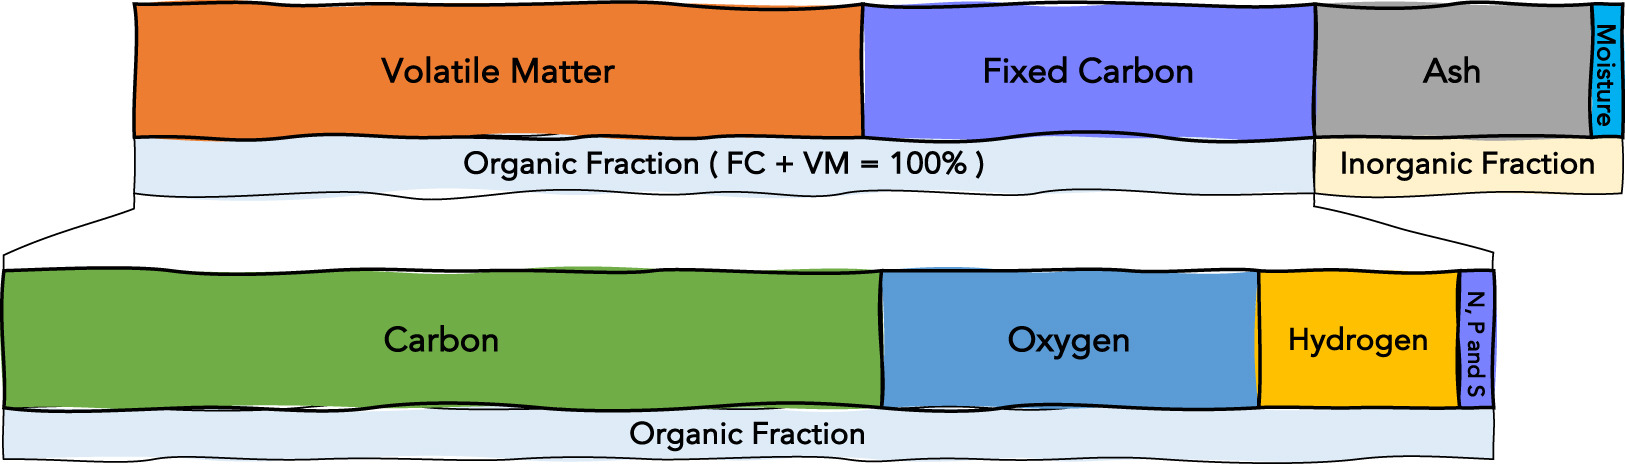
\includegraphics[width=0.8\linewidth]{Abbildungen/gr3_lrg.jpg}
    \caption{Scheme to the chemical composition of biochars.}
    \label{fig:2.1.1.1}
\end{figure}

\begin{table}[H]
\centering
\caption{Elemental composition of biochar. \cite{Sajjadi2019}}
\label{tab:Elemental composition of biochar}

\small
\begin{tabular}{l c c}
\toprule
\textbf{Element} & \textbf{Symbol} & \textbf{Typical content (\%)} \\
\midrule
Carbon   & C & 40--70 \\
Oxygen   & O & 10--45 \\
Hydrogen & H & 1--5 \\
Nitrogen & N & 0--3 \\
Sulfur   & S & $<$1 \\
\bottomrule
\end{tabular}
\end{table}

\newpage
The content of biochar is significantly influenced by the bulk composition of the feedstock. Wood and crop-derived biochar has higher carbon content compared to manure-derived biochar due to its higher lignin content, whereas manure-based biochar has higher nutrient, because it has already rich inorganic elements \cite{Ippolito2020BiocharCharacteristics}. For this reason, manure-derived biochar contains high amount of ash. 


\begin{table}[H]
\centering
\caption{Biochar chemical characteristic. PT = pyrolysis temperature; PY = pyrolysis yield; VM = volatile matter; A = ash content. \cite{Domingues2017} \cite{tomczyk-2020}.}
\label{tab:biochar_properties_elemental}

\small
\resizebox{\textwidth}{!}{%
\begin{tabular}{l c c c c c c c c c c c}
\toprule
\textbf{Biomass} & \textbf{PT} 
& \textbf{PY} & \textbf{pH} & \textbf{VM} & \textbf{A}
& \multicolumn{4}{c}{\textbf{Elemental composition (\%)}} 
& \multicolumn{2}{c}{\textbf{Atomic ratio}} \\
\cmidrule(lr){7-10} \cmidrule(lr){11-12}
& \textbf{($^\circ$C)} 
& \textbf{(\%)} & & \textbf{(\%)} & \textbf{(\%)}
& \textbf{C} & \textbf{H} & \textbf{S} & \textbf{O} 
& \textbf{H/C} & \textbf{O/C} \\
\midrule

Chicken manure       & 350 & 69.7 & 9.7  & 36.9 & 52.0 & 31.2 & 1.97 & 0.31 & 10.9 & 0.76 & 0.26 \\
                     & 450 & 63.0 & 10.2 & 30.6 & 55.3 & 27.2 & 1.92 & 0.44 & 11.4 & 0.85 & 0.31 \\
                     & 750 & 55.9 & 11.7 & 26.5 & 56.4 & 24.7 & 0.67 & 0.29 & 16.3 & 0.32 & 0.49 \\
\midrule

Eucalyptus sawdust   & 350 & 42.5 & 5.9  & 36.9 & 0.9  & 70.4 & 3.81 & 0.02 & 24.0 & 0.65 & 0.26 \\
                     & 450 & 36.0 & 8.0  & 28.5 & 0.7  & 78.6 & 3.42 & 0.01 & 16.6 & 0.52 & 0.16 \\
                     & 750 & 28.2 & 9.7  & 6.5  & 1.1  & 90.9 & 1.52 & 0.04 & 5.6  & 0.20 & 0.05 \\
\midrule

Coffee husk          & 350 & 43.5 & 9.7  & 34.6 & 12.9 & 60.5 & 3.92 & 0.09 & 19.5 & 0.78 & 0.24 \\
                     & 450 & 37.7 & 9.8  & 26.2 & 12.9 & 61.3 & 3.65 & 0.10 & 19.0 & 0.71 & 0.23 \\
                     & 750 & 31.6 & 9.9  & 17.6 & 19.6 & 66.0 & 1.57 & 0.23 & 9.8  & 0.29 & 0.11 \\
\midrule

Sugarcane bagasse    & 350 & 37.5 & 7.2  & 35.0 & 1.9  & 74.7 & 4.26 & 0.03 & 17.9 & 0.68 & 0.18 \\
                     & 450 & 33.2 & 8.8  & 24.0 & 2.1  & 81.6 & 3.66 & 0.05 & 11.3 & 0.54 & 0.10 \\
                     & 750 & 26.9 & 9.7  & 7.7  & 2.2  & 90.5 & 1.64 & 0.06 & 4.3  & 0.22 & 0.04 \\
\midrule

Pine bark            & 350 & 59.6 & 7.8  & 38.5 & 8.3  & 67.6 & 3.73 & 0.01 & 28.7 & 0.66 & 0.32 \\
                     & 450 & 49.3 & 8.3  & 29.3 & 7.9  & 75.2 & 2.74 & 0.02 & 24.7 & 0.44 & 0.25 \\
                     & 750 & 38.9 & 9.9  & 6.0  & 14.5 & 86.3 & 1.16 & 0.04 & 19.1 & 0.16 & 0.17 \\
\bottomrule

\end{tabular}%
}

\vspace{0.3em}
\end{table}

\label{Properties of Biochar}
\subsubsection*{Functional Groups and pH}
The properties of biochar are closely related to its functional groups, mainly oxygen-containing groups (Table~\ref{tab:surface-functional-groups} and Figure~\ref{fig:2.1.1.2}), which are the major active sites on surface of biochar that influence the adsorption ability of biochar \cite{Sajjadi2019}. 

\begin{table}[h]
\centering
\caption{Oxygen-containing surface functional groups in biochar}
\label{tab:surface-functional-groups}
\begin{tabular}{l}
\toprule
\textbf{Surface functional group} \\
\midrule
Carbonyl \\
Quinone \\
Ether \\
Carboxylic anhydride \\
Lactone \\
Carboxylic acid \\
Phenol \\
Intercalated oxygen \\
\bottomrule
\end{tabular}
\end{table}

\begin{figure}[ht!]
    \centering
    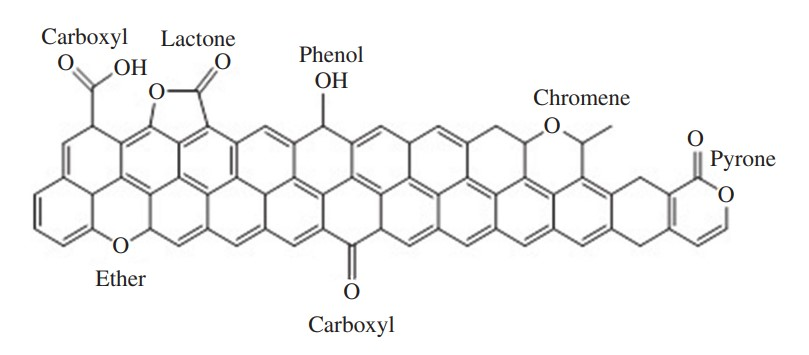
\includegraphics[width=0.8\linewidth]{surface functional group.jpg}
    \caption{Oxygen-containing surface functional group.}
    \label{fig:2.1.1.2}
\end{figure}

\vspace{0.3em}


\newpage
The oxygen-containing functional group is profoundly impacted by the pyrolysis temperatures. At low pyrolysis temperatures, the acidic functional groups are relatively abundant, making the produced biochars tend to be acidic, hydrophilic, and polar, whereas the biochars tend to be alkaline, hydrophobic, and nonpolar at higher pyrolysis temperatures, as the acidic functional groups are gradually eliminated and the concentratio of carbonat, ash, and inorganic alkali salts is higher \cite{Sajjadi2019} \cite{Tomczyk2020}. 

\vspace{0.3em}

In addition to oxygen-containing groups, biochars made from nitrogen-rich feedstocks like manure or sewage sludge may contain nitrogen-containing groups (such pyrrolic and pyridinic N), which provide additional Lewis base sites important for the adsorption of acidic contaminants.


%During pyrolysis, under increasing temperature, the higher degree of carbonization reduces the atomic ratios of H/C, O/C,and N/C, followed by a reduction in the abundances of carboxylic, hydroxyl, and amino groups.

%The O/C value represents the quantity of superficial polar functional groups and the hydrophilicity of BC, whereas the H/C value indicates the aromatization of the organic structure (Fang et  al. 2014, Han et  al. 2017). During pyrolysis, under increasing temperature, the higher degreeof carbonization reduces the atomic ratios of H/C, O/C, and N/C, followed by a reduction in the abundances of carboxylic, hydroxyl, and amino groups. Different elements of BC are (usually) determined by dry combustion, 




%whereas these elements respectively contribute to different functional groups that influence and determine other chemical properties, such as pH and nutrient value, as well as cation exchange capacity \cite{Munzeiwa2025BiocharBaselinePotential}. Oxygen contributes in forming surface functional groups, including hydroxyl and carboxyl that influence the pH value and cation exchange capacity of biochar. On the other hand, sulfur and phosporus content still associated with the pH value and CEC, while nitrogen content associated with the nutrient value \cite{Munzeiwa2025BiocharBaselinePotential}. 

%Oxygen content influences the resulting surface functionalities (e.g., hydroxyl, carboxyl, etc.) resulting in acidic biochar and improved cation exchange Content courtesy of Springer Nature, terms of use apply. Munzeiwa et al. Discover Water (2025) 5:77 Page 6 of 48 capacity (CEC). Biomass with higher oxygen content tends to have a lower carbon content but enhanced pore structure and surface area [69]. The elemental ratios C/H, C/O, and H/O can be used as indices for baseline potential, energy content, and environmental consequences of the biomass [160]. Whereas a higher C/H ratio predisposes biochar characterized by high aromaticity and stable graphic microstructure, a low C/H ratio indicates highly aliphatic biomass that is susceptible to decomposition [160]. A higher C/O ratio shows low oxygen content, resulting in more carbonization and lower reactivity [161].
%Nitrogen content influences the diversity of chemical moieties of the surface by contributing to the formation of functional groups such as amines, amides, pyrroles, pyridines, and nitriles, while sulfur contributes to thiols, sulfides, sulfonic acids, and sulfates, and P forms phosphates and phosphites which influence the pH and CECs of the resulting biochar [99, 100].

%\label{Properties of Biochar}
%\subsubsection*{pH}

%The pH of biochar is one the crucial chemical property in order to determine its application involving soil, since soil has varying levels of acidity and alkalinity. Acidic 


%Surface functional groups are an important chemical characteristic of biochar because they strongly influence its reactivity, interaction with water, nutrient retention, and adsorption behaviour. Although biochar is mainly described as a carbon-rich material, its surface is not chemically uniform. Instead, it contains different functional groups attached to the carbon matrix, particularly oxygen-containing groups such as hydroxyl, carboxyl, carbonyl, phenolic, lactone, ether, and quinone groups. Depending on the feedstock material and the production conditions, biochar may also contain nitrogen-, phosphorus-, or sulfur-containing functional groups, although these are usually present in smaller amounts compared with oxygen-based groups

\label{Properties of Biochar}
\subsubsection*{Specific Surface Area and Porosity}

The physical properties of biochar are primarily characterized by its specific surface area and porosity, which determine the reactivity and adsorption capacity of biochar \cite{Ingle2024}. Biochar displays high porosity with pores ranging from micro- (<2 nm) to macropores (>50 nm) \cite{Tomczyk2020} \cite{Sajjadi2019}, while the size of its specific surface area also vary. They are influenced by BC feedstock, pyrolysis temperature, and the activation process \cite{Sajjadi2019}. High pyrolysis temperature stimulates micropores formation, leading to larger specific surface area \cite{Sajjadi2019}. Micropores are also mainly formed from cellulose-enriched feedstock, whereas macropores are mainly observed in lignin-enriched feedstocks based biochar. The specific surface area and porosity of crop-residue-derived biochar are much bigger compared to those of animal-li-derived biochar, which is caused by the higher carbon content of plant-derived biochar \cite{Tomczyk2020} \cite{Sajjadi2019}. 

\begin{table}[H]
\centering
\caption{Specific surface area of different biochars. PT = pyrolysis temperature; SSA = specific surface area \cite{Tomczyk2020}.}
\label{tab:biochar_ssa_selected}

\small
\resizebox{0.75\textwidth}{!}{%
\begin{tabular}{l c c l}
\toprule
\textbf{Biomass feedstock} & \textbf{PT ($^\circ$C)} & \textbf{SSA (m$^2$/g)} & \textbf{Reference} \\
\midrule

Sugarcane bagasse & 400 & 0.8  & Ding et al. \cite{Ding2014BagasseBiochar} \\
Rapeseed plant    & 400 & 16.0 & Karaosmanoglu et al. \cite{Karaosmanoglu2000RapeseedCake} \\
Cow manure        & 400 & 2.5  & Kolodynska et al.\cite{Kolodynska2012BiocharMetalIons} \\
Pig manure        & 400 & 15.6 & Kolodynska et al.\cite{Kolodynska2012BiocharMetalIons} \\

\bottomrule
\end{tabular}%
}

\vspace{0.3em}
\end{table}

As example, figure~\ref{fig:bgr_biochar} illustrates the surface area and porosity of  plant-based charcoal and biochar. The charcoal and gasification coke produced from beech wood exhibit a porous surface structure, which is associated with a larger accessible surface area. By contrast, the flash-pyrolysis coke produced from spruce wood is covered by a resin layer, which reduces the accessible surface and limits the development or exposure of pores. 

\begin{figure}[ht!]
    \centering
    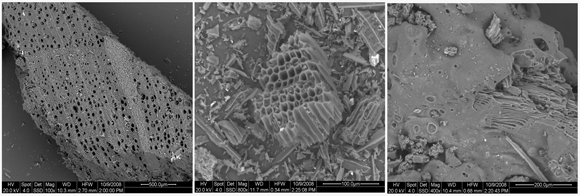
\includegraphics[width=1\textwidth]{Abbildungen/Biokohle.png}
    \caption{Surface area and porosity of charcoal from beech wood (left), gasification coke from beech wood (middle) and flash-pyrolisis coke from spruce wood (right)\cite{BGRBiochar}}
    \label{fig:bgr_biochar}
\end{figure}

\vspace{0.3em}

\subsubsection{Physical Activation of Biochar}

Physical activation refers to a method to produce activated biochar that has a larger surface area, wide range of functional groups and a more
uniform pore size distribution, leading to improvement on adsorption capacity of biochar. The most established and practically used physical approach is to activate the biochar by treating it with oxidizing agent, mainly steam and carbon dioxide, at temperature above 700°C. During this gaseous activation, oxidizing agents penetrate and gasify the structure of biochar consisting mainly from carbon atom, resulting in newly open and wider blocked pores. Therefore, activated biochar has higher internal surface areas and more oxygen functional groups as adsorption active sites \cite{sajjadi-2018}. 

\label{Physical Activation of Biochar}
\subsubsection*{Steam Activation}



Together with carbon dioxide 









%Steam activation is one of the oldest and most well-established methods for the physical activation of carbonaceous materials (Marsh and Reinoso, 2006). The process involves exposing biochar to superheated steam, typically at temperatures ranging from 700 to 900°C, for durations spanning from 30 minutes to several hours (Demiral et al., 2011; Girgis et al., 2011; Han et al., 2013). The smaller molecular size of water compared to CO₂ is a fundamental advantage of steam as an activating agent, as it facilitates deeper diffusion into the internal pore network of the biochar, inducing a faster and more thorough reaction throughout the material (Dalai and Azargohar, 2007). Unlike air activation, the reaction between steam and carbon is endothermic in nature, which makes it inherently more controllable and better suited for the activation of carbons with high surface activity (Sajjadi et al., 2018).
%The overall reaction mechanism of steam activation with biochar involves several sequential and concurrent steps, beginning with the chemisorption of water molecules onto active carbon surface sites (Lussier et al., 1998). In this initial step, oxygen from the water molecule is transferred to the carbon surface, forming a surface oxide complex while releasing hydrogen gas. This surface oxide may subsequently desorb from the carbon surface as carbon monoxide, regenerating an active carbon site. The carbon monoxide produced can further participate in the gasification process by scavenging additional surface oxide species to yield carbon dioxide. A water-gas shift reaction then proceeds in parallel, in which water vapor is decomposed into carbon dioxide and hydrogen gas (Sattar et al., 2014; Ferreira et al., 2017). The hydrogen produced can go on to further activate the carbon surface or inhibit gasification depending on local concentration. Hydrogen produced during these reactions has been shown to adsorb onto active carbon sites, forming stable surface hydrogen complexes that effectively block and deactivate those sites, thereby inhibiting further gasification (Lussier et al., 1998). Hydrogen adsorbed onto carbon surfaces requires temperatures as high as 1500°C for complete desorption, as detailed by Redmond and Walker (1960), meaning that the inhibitory effect of hydrogen is a persistent feature of the steam activation process that must be carefully managed through control of activation temperature and steam flow rate. Hüttinger (Hermann and Hüttinger, 1986) identified three possible mechanisms by which hydrogen inhibits steam gasification: dissociative hydrogen adsorption onto free active carbon sites, reverse oxygen exchange between hydrogen and surface oxides, and the scavenging of surface oxides by hydrogen gas.

\newpage
\label{Physical Activation of Biochar}
\subsubsection*{\textbf{CO$_2$} Activation}

The mechanism of biochar activation with carbon dioxide 






The mechanism of char (C) activation with CO2
involves the Boudouard reaction (C + CO2 ↔ 2CO). In this
process, CO2 undergoes dissociative chemisorption on the
carbon surface to form a surface oxide and carbon mon-
oxide as shown in R12. The surface oxide, C(O), is sub-
sequently desorbed from the surface, further developing
the pore structure (R13). CO in the gaseous product can
also be adsorbed on the carbon active site and retards the
gasification (R14).



\newpage
\subsubsection{Sulfur Loading of Biochar}

Sulfur loading refers to a process for increasing the sulfur content in biochar by exposing it to sulfur compounds, primarily hydrogen sulfide. The concept of sulfur loading is identical to the hydrogen sulfide removal process, which lets elemental sulfur to be adsorbed on the surface of biochar. In this process, the elemental sulfur is formed through the partial oxidation of hydrogen sulfide by oxygen in air \cite{Lin2025H2SOxidationPETBiochar}. Full oxidation is avoided to prevent the formation of unwanted sulfur dioxide ($SO$_2$) or sulfate ($SO$_4^{2-}$).

\begin{equation}
H_2S + \frac{1}{2}O_2 \rightarrow S + H_2O
\end{equation}

This process is favored for activated biochar due to its larger specific surface area and modifiable porosity compared to pristine biochar \cite{Lin2025H2SOxidationPETBiochar}. 

\vspace{0.3em}



%Sulfur loading of biochar refers to the enrichment of biochar with sulfur-containing species through adsorption, impregnation, or reaction with sulfur compounds. This modification is commonly applied to improve the chemical functionality of biochar and to expand its potential use as a soil amendment, fertiliser, or adsorbent material. In general, pristine biochar already contains a certain amount of sulfur depending on the original feedstock. However, the sulfur content is often relatively low compared with other major elements such as carbon, oxygen, potassium, calcium, and phosphorus. The total sulfur content of biochar is strongly influenced by feedstock type. 

%Sulfur loading can be carried out by exposing biochar to sulfur-containing gases, especially hydrogen sulfide (H$_2$S), or by treating it with sulfur-containing solutions. One important example is the use of activated biochar to remove H$_2$S from biogas streams. H$_2$S is a toxic and corrosive gas commonly produced during anaerobic digestion, and its removal is necessary to prevent equipment corrosion and environmental problems. Biochar can act as an adsorbent for H$_2$S due to its porous structure, surface area, pH, mineral content, and surface functional groups. In addition to physical adsorption, biochar can also promote the oxidation of H$_2$S into other sulfur forms, such as elemental sulfur and sulfate. These reactions are influenced by the surface chemistry of the biochar, including oxygen-containing functional groups, aromatic carbon structures, and catalytic elements such as iron and calcium.

%The effectiveness of sulfur loading depends strongly on the properties of the biochar. A higher surface area and well-developed pore structure can provide more adsorption sites for sulfur compounds. The pyrolysis temperature and activation process also play important roles because they influence the surface area, pore volume, pH, and the stability of functional groups. For example, steam activation can increase the surface area and microporosity of biochar, making it more suitable for gas adsorption. In the study by Zhang et al., sulfur-enriched biochar was produced by passing landfill biogas through a packed column containing activated biochar. The biochar used in this process was produced from anaerobically digested solid dairy manure and then steam activated. After exposure to H$_2$S-containing gas, the resulting sulfur-loaded biochar, referred to as SulfaChar, showed a sulfur content of 36.5%, compared with only 2.7% in the original biochar. This confirms that biochar can adsorb and retain a significant amount of sulfur from H$_2$S gas.

%Sulfur-loaded biochar is interesting not only as a gas-cleaning material but also as a potential fertiliser. Sulfur is an essential plant nutrient because it is involved in protein synthesis, enzyme activity, and chlorophyll formation. When sulfur is retained in biochar as plant-available forms such as sulfate, the material may function as a slow-release sulfur source in soil. Zhang et al. reported that SulfaChar increased corn biomass and enhanced the uptake of sulfur as well as other macro- and micronutrients, including nitrogen, phosphorus, potassium, calcium, magnesium, zinc, manganese, and boron. This suggests that sulfur-loaded biochar can act either as a direct nutrient supplier or as a carrier material that improves nutrient uptake efficiency.

%Biochar, enriched with sulfur, has recently emerged as a promising alternative in sustainable agricultural practices, particularly as a means of enhancing soil fertility. This approach addresses the dual challenge of managing environmental contamination and optimizing resource utilization. Conventional fertilizers, although effective in nutrient delivery, often pose risks to ecosystems due to their propensity for nutrient runoff and chemical leaching, contributing to ecological imbalance. Hence, biochar enriched with sulfur offers an eco-friendly and resource-efficient solution by improving nutrient retention capacity, promoting soil organic matter content, and subsequently enhancing plant productivity. On the other side, sulfur enrichment of biochar can be achieved through the adsorption of hydrogen sulfide ($H_2S$), a highly toxic and corrosive gaseous contaminant commonly produced during the anaerobic digestion of organic waste for methane generation. Recent studies indicate that biochar possesses substantial potential as an effective adsorbent for $H_2S$ removal from biogas, thereby not only mitigating the environmental hazards associated with $H_2S$ emissions but also creating a value-added sulfur-enriched biochar suitable for agricultural use. 

\subsubsection{Utilization of Biochar}

Biochar has broad application depending to its modifications. 

\newpage
\setresponsible{Surya Salim}
\subsection{Pyrolisis}

%https://www.intechopen.com/chapters/78772
%https://www.intechopen.com/books/10862
%https://www.mdpi.com/1996-1073/5/12/4952
\subsubsection{Definition and principle of pyrolysis}
Pyrolysis is one of the most widely used thermochemical methods for converting biomass and producing biochar. It involves the thermal decomposition of organic material under an inert atmosphere, in the absence of oxygen, yielding three primary products: char, bio-oil, and syngas. Bio-oil is a complex liquid mixture composed of hundreds of oxygenated compounds, which can be further upgraded using specialized catalysts to produce biofuels or value-added chemicals. During pyrolysis, the complex molecular structure of biomass is broken down into smaller, simpler components, resulting in the formation of both a vapor phase and a solid phase \cite{Dufour2016}.

\subsubsection{Slow versus Fast Pyrolysis}
Pyrolysis of biomass is broadly classified into three modes: slow, intermediate, and fast pyrolysis. The key parameters governing this classification, which also serve as the primary operating conditions, are the heating rate, temperature, and vapor residence time \cite{Vuppaladadiyam2022}.
\vspace{0.3em}
\newline
Fast pyrolysis is characterized by very high heating rates (typically exceeding 100 °C/s), short vapor residence times of less than 2 seconds, and moderate temperatures ranging from 500 to 700 °C. These conditions promote rapid thermal decomposition, favoring the production of liquid products — particularly bio-oil — which can reach yields of up to 70–75 wt.\% \cite{Lehmann2015,Luque2016}.
\vspace{0.3em}
\newline
In contrast, slow pyrolysis operates at lower heating rates (0.1–1 °C/s), longer residence times (minutes to hours), and temperatures typically ranging from 300 to 700 °C. Under these conditions, volatile compounds remain in contact with the solid phase for longer periods, enabling secondary reactions that promote char formation. This mode of pyrolysis is preferred when the primary objective is to maximize biochar yield, a process also referred to as carbonization \cite{Lehmann2015,Pahnila2023}.
As a result of these process differences, slow pyrolysis is primarily employed for biochar production, whereas fast pyrolysis is optimized for bio-oil production. The prolonged interaction between vapors and the solid phase in slow pyrolysis enhances carbonization, leading to higher solid yields. Consequently, slow pyrolysis is the preferred thermochemical conversion route when the objective is to produce stable, carbon-rich biochar with well-developed structural properties.

\begin{table}[H]
\centering
\caption{Comparison of slow and fast pyrolysis for biomass (adapted from \textcite{Tan2021})}
\label{tab:pyrolysis_comparison}
\small
\begin{tabular}{p{2.5cm} p{6cm} p{6cm}}
\hline
\textbf{Features} & \textbf{Slow Pyrolysis} & \textbf{Fast Pyrolysis} \\
\hline
Temperature (°C) & 300–700 & 600–1000 \\[3pt]
Heating rates (°Cmin$^{-1}$) & 0.1–10 & 10–10000 \\[3pt]
Aeration & Oxygen-free or limited & Oxygen-free \\[3pt]
Residence Time & Minutes–hours & Seconds \\[3pt]
Target product & Biochar & Bio-oil \\[3pt]
Advantages & -The highest yield of biochar. \newline -Can accept a wide range of particle size. & -A higher yield of bio-oil. \\[3pt]
Disadvantages & Further treatment of gases is needed due to high CO concentrations & -Low biochar yield. \newline -Fine particle of biomass feed (1–2mm) is required. \newline -Prefer biomass with low moisture content ($<$10\%) \\[3pt]
\hline
\end{tabular}
\end{table}


\subsubsection{Thermal decomposition of biomass components}
Biomass subjected to pyrolysis typically consists of a mixture of organic and inorganic constituents, including lignocellulosic components (cellulose, hemicellulose, and lignin), as well as proteins, lipids, and mineral matter. The thermal decomposition behavior of these constituents plays a crucial role in determining the yield and properties of the resulting biochar \cite{Yang2007,Wen2021}.

\vspace{0.3em}

The lignocellulosic fraction exhibits distinct thermal decomposition characteristics. Hemicellulose is the least thermally stable component, decomposing at relatively low temperatures, typically between 150 °C and 300 °C. Cellulose decomposes at slightly higher temperatures, generally in the range of 320 °C to 400 °C, and is characterized by a sharp and narrow degradation profile. In contrast, lignin decomposes over a much broader temperature range, from approximately 250 °C up to 600 °C or higher, owing to its complex aromatic structure \cite{ElSayed2023,Chen2026}.

\vspace{0.3em}

The overall pyrolysis process can be divided into several stages. At temperatures below approximately 220 °C, moisture evaporation dominates. Between 220 °C and 400 °C, rapid devolatilization occurs, primarily due to the decomposition of hemicellulose and cellulose. At higher temperatures, above 400 °C, lignin degradation and carbonization become dominant, leading to the formation of a carbon-rich solid residue \cite{Yang2005,ElSayed2023}. Notably, compared to cellulose and hemicellulose, lignin decomposes more slowly and contributes significantly to char formation owing to its high thermal stability and complex aromatic structure. Consequently, lignin is considered the primary precursor for biochar formation during pyrolysis \cite{Chen2022}.

\vspace{0.3em}

In addition to lignocellulosic components, digestate-based feedstocks contain proteins, lipids, and inorganic minerals, which further influence pyrolysis behavior. Proteins decompose to form nitrogen-containing compounds, that affect the nitrogen content of the resulting biochar\cite{Navarro2025}. Lipids tend to promote the formation of liquid products, while inorganic minerals can act as catalysts, altering reaction pathways and influencing pore development. Furthermore, interactions between these components during pyrolysis can lead to non-additive effects, resulting in complex product distributions and structural characteristics of biochar \cite{Puri2024,Kebelmann2013}.

\begin{table}[H]
\centering
\caption{Biomass components and their role during pyrolysis\cite{Chen2022,Armanu2024,Puri2024}}
\label{tab:biomass_components}
\small
\begin{tabular}{p{2cm} p{2.2cm} p{1.8cm} p{3.2cm} p{2.5cm} p{3cm}}
\hline
\textbf{Component} & \textbf{Typical Decomposition Temperature} & \textbf{Thermal Stability} & \textbf{Main Role During Pyrolysis} & \textbf{Effect on Char Formation} & \textbf{Key Notes} \\
\hline
Hemicellulose & $\sim$150–300°C & Low & Decomposes early $\rightarrow$ releases CO$_2$, volatiles & Very low & Produces mostly gases and light compounds; little solid residue \\[6pt]

Cellulose & $\sim$320–400°C & Medium & Rapid depolymerization $\rightarrow$ volatiles (e.g. levoglucosan) & Moderate & Can contribute to char under certain conditions\cite{Armanu2024} \\[6pt]

Lignin & $\sim$250–600°C (wide range) & High & Slow decomposition $\rightarrow$ aromatic structures & High (dominant) & Main precursor for stable biochar \\[6pt]

Proteins & $\sim$200–500°C & Medium & Decompose $\rightarrow$ NH$_3$, N-compounds & Indirect & Increase nitrogen content in biochar \\[6pt]

Lipids (fats) & $\sim$300–500°C & Medium & Crack into hydrocarbons and oils & Low / negative & Promote bio-oil formation $\rightarrow$ reduce char yield \\[6pt]

Mineral matter (ash) & Non-decomposing (inorganic) & Very high & Catalyzes reactions & Indirect (can increase or decrease) & Alters decomposition pathways and pore structure \\
\hline
\end{tabular}
\end{table}

\subsubsection{Influence of Pyrolysis Condition on Bichar Properties}
\label{Influence pyrolysis condition}
\subsubsection*{Effect of Temperature on Biochar}
\label{subsubsec:Effect of Temperature on Biochar}
Pyrolysis temperature is one of the most influential parameters governing the physicochemical properties of biochar. It directly affects the extent of thermal decomposition, carbonization, and structural transformation of biomass, thereby determining the resulting biochar yield, elemental composition, porosity, and stability \cite{Lataf2022}.

\vspace{0.3em}

With increasing pyrolysis temperature, biochar yield generally decreases due to the enhanced release of volatile compounds, such as gasses and condensable vapors. At lower temperatures, incomplete decomposition leads to higher retention of solid mass, whereas higher temperatures promote devolatilization and reduce the remaining char fraction \cite{zhang-2014}.

\vspace{0.3em}

Simultaneously, increasing pyrolysis temperature leads to a higher degree of carbonization, reflected in a rising carbon content and a concurrent decrease in hydrogen and oxygen content, resulting in a more aromatic and condensed carbon structure. Consequently, biochar produced at higher temperatures exhibits enhanced thermal stability and resistance to degradation \cite{zhang-2014,zhang-2022,224pyrolysistemp}.

\vspace{0.3em}

In addition, elevated pyrolysis temperatures promote the development of pore structures due to the progressive release of volatile matter. This results in increased surface area and porosity, which are important for adsorption-related applications. However, excessively high temperatures may also lead to pore widening or structural collapse, depending on the feedstock and process conditions \cite{tomczyk-2020,ghorbani-2022}.

\vspace{0.3em}

Overall, pyrolysis temperature governs a fundamental trade-off between biochar yield and quality: lower temperatures favor higher yields but produce less stable and less carbonized materials, while higher temperatures enhance structural stability, carbon content, and porosity at the expense of reduced yield.


\subsubsection*{Effect of Heating Rate on Biochar}

Heating rate is one of the operational parameters that must be defined in pyrolysis. It influences thermal decomposition pathways, volatile release, and the physicochemical properties of the resulting biochar. As a general rule of thumb, slow heating rates promote gradual devolatilization and prolong the interaction between volatile compounds and the solid phase, thereby favoring secondary charring reactions and enhancing solid carbon formation \cite{awad-2024,brunner-1980}.

\vspace{0.3em}

Compared to rapid heating conditions, low heating rates are commonly associated with higher char yields and improved structural ordering of biochar. Slow pyrolysis conducted at heating rates in the range of approximately 10–30 °C/min has been widely reported as suitable for maximizing biochar production \cite{awad-2024}.

\vspace{0.3em}

In addition, heating rate can influence pore development and carbon structure formation. Previous studies have shown that slowly carbonized biomass may exhibit larger micropore volumes and more developed surface characteristics compared to rapidly heated samples \cite{awad-2024,song-2025}.
In the present study, a constant heating rate of 10 °C/min was selected to ensure controlled thermal decomposition under slow pyrolysis conditions and to promote the formation of stable, carbon-rich biochar.


\subsubsection*{Effect of Residence Time on Biochar}
Residence time is another important operational parameter in pyrolysis, as it influences the extent of devolatilization, carbonization, and structural transformation of biomass during thermal decomposition. Longer residence times allow biomass to remain at elevated temperatures for extended periods, thereby promoting further decomposition of volatile compounds and the formation of more condensed carbon structures \cite{leng-2018,wang-2019}. Several studies have reported that increasing residence time can reduce biochar yield due to the continued release of volatile matter and secondary cracking reactions. At the same time, extended residence times are generally associated with higher pH values, increased ash content, and greater aromaticity of the resulting biochar \cite{sun-2016,wijitkosum-2023}.

\vspace{0.3em}

Residence time also affects the physicochemical structure of biochar, including surface area and pore development. Moderate residence times may enhance pore formation and surface characteristics, whereas excessively long residence times can lead to pore widening or partial structural collapse \cite{wang-2019}. However, compared to pyrolysis temperature, the influence of residence time on biochar properties is often less pronounced. Previous studies have reported that pyrolysis temperature is generally the dominant parameter governing biochar characteristics, while the effects of residence time are comparatively minor \cite{wang-2020, zhao-2017}.

\vspace{0.3em}

In the present study, a constant residence time of 1 hour was selected to ensure sufficient devolatilization and stable carbonization under slow pyrolysis conditions. Although pyrolysis temperature was the principal variable investigated, the selected heating rate and residence time also contributed to the final physicochemical properties of the produced biochars.

\vspace{0.3em}

The physicochemical properties of biochar are strongly governed by pyrolysis conditions such as temperature, heating rate, and residence time. These process parameters directly influence the elemental composition, aromaticity, pore structure, surface functionality, and stability of the resulting biochar, thereby determining its suitability for specific applications \cite{luo-2024,tomczyk-2020}.
For soil amendment applications, biochar produced at relatively lower pyrolysis temperatures generally retains a higher proportion of oxygen-containing functional groups and volatile matter, which may enhance nutrient exchange capacity and microbial interactions in soil. In contrast, biochar produced at higher temperatures typically exhibits greater aromaticity, higher carbon stability, and increased resistance to microbial degradation, making it more suitable for long-term carbon sequestration and persistent soil conditioning \cite{lu-2021,nogues-2023,pokharel-2025}.
Pyrolysis temperature also significantly influences pore development and surface area. Elevated temperatures promote devolatilization and the formation of more developed porous structures, which are beneficial for adsorption-related applications such as wastewater treatment, gas purification, and contaminant removal. Higher-temperature biochars generally possess larger surface areas and improved adsorption performance due to increased aromaticity and pore formation \cite{loebsack-2025,luo-2024}.
In addition, biochar characteristics relevant to soil improvement — including water-holding capacity, cation exchange capacity, pH, and microbial interactions — are strongly dependent on pyrolysis conditions. Several studies have reported that biochar produced within intermediate-to-high temperature ranges may significantly improve soil aggregation, water retention, and long-term soil carbon conservation \cite{ghorbani-2022,kabir-2023,shyam-2025}.
Therefore, optimization of pyrolysis conditions is essential to tailor biochar properties for targeted applications. Lower-temperature biochars may be more favorable for nutrient-related and biologically active soil applications, whereas higher-temperature biochars are generally preferred for adsorption processes, contaminant remediation, and long-term carbon sequestration.

\subsubsection{Relevance of Pyrolysis for digestate-derived biochar}
\label{subsubsec:digestate-pyrolysis relevance}
Digestate-derived biochar differs significantly from biochar produced from conventional lignocellulosic biomass such as wood, straw, or agricultural residues. Digestates represent complex biomass matrices containing partially degraded organic matter resulting from anaerobic digestion, as well as elevated mineral and ash contents. In addition to residual lignocellulosic structures, digestates may contain proteins, lipids, and inorganic compounds, all of which influence thermal decomposition behaviour during pyrolysis \cite{kujawska-2026,sarkar-2024}.

\vspace{0.3em}

Due to this heterogeneous composition, the physicochemical properties of digestate-based biochar are strongly dependent on pyrolysis temperature. Pyrolysis temperature governs the extent of devolatilization, carbonization, aromatization, and pore development, thereby determining the resulting yield, elemental composition, stability, and surface characteristics of biochar \cite{kujawska-2026, manya-2012}.

\vspace{0.3em}

At relatively low pyrolysis temperatures of around 400 °C, carbonization remains incomplete and the resulting biochar typically retains a larger proportion of volatile matter and oxygen-containing functional groups. Consequently, low-temperature biochars often exhibit higher yields, greater chemical reactivity, and improved nutrient exchange capacity. However, their carbon structure is generally less aromatic and less resistant to microbial degradation \cite{wystalska-2021}.

\vspace{0.3em}

Intermediate pyrolysis temperatures of around 500 °C are commonly regarded as a transition region between incomplete carbonization and the formation of more condensed aromatic carbon structures. Within this temperature range, biochar may exhibit a balance between yield retention and improved physicochemical properties, such as thermal stability and pore development \cite{alghashm-2023,kujawska-2026}.

\vspace{0.3em}

At higher pyrolysis temperatures of around 600 °C, devolatilization and carbonization become more pronounced, resulting in biochar with increased aromaticity, enhanced thermal stability, and more developed pore structures. Elevated temperatures also promote the elimination of hydrogen- and oxygen-containing functional groups, leading to more carbon-rich and chemically stable biochar materials \cite{kujawska-2026,wystalska-2021}.

\vspace{0.3em}

Several studies have reported that increasing pyrolysis temperature generally reduces biochar yield due to the enhanced release of volatile compounds. However, digestate-derived biochars may exhibit more complex behavior owing to their elevated mineral and ash contents. Inorganic components such as potassium, calcium, magnesium, and phosphorus may catalytically influence pyrolysis reactions and alter char formation pathways, resulting in deviations from conventional lignocellulosic biomass trends\cite{kujawska-2026,wang-2023}.

\vspace{0.3em}

In the present study, pyrolysis temperatures of 400 °C, 500 °C, and 600 °C were selected to investigate the transition from partially carbonized digestate-derived biochar toward more thermally stable and aromatic carbon structures. Particular attention was given to the relationship between pyrolysis temperature and biochar yield, elemental composition, and surface morphology.


\newpage
\subsection{Calorific Value (HHV and LHV)}

\subsubsection*{Definition}
The two principal calorific descriptors of a solid fuel are the \textbf{higher heating value} (HHV; also termed Brennwert, gross calorific value, GCV, or $H_0$) and the \textbf{lower heating value} (LHV; also termed Heizwert, net calorific value, NCV, or $H_u$).
\begin{itemize}
    \item \textbf{HHV (Brennwert /  $H_0$ / GCV )} is defined as the absolute value of the specific energy of combustion, in joules, of unit mass of a fuel burned in oxygen in a calorimetric bomb under specified standard conditions, with the resulting water of combustion fully condensed to the liquid state at the reference temperature of 25°C \cite{iso18125_2017,din51900_2023,astm_d5865_2019}. HHV is therefore measured at constant volume.
    \item \textbf{LHV (Heizwert / $H_u$ / NCV)} is the corresponding heat of combustion calculated under conditions where the water of combustion remains in the vapor state. LHV at constant pressure is the operative quantity used in practical fuel applications (boilers, gasifiers, combustors), since flue gases generally leave the system above the dew point \cite{iso18125_2017, din51900_old,van-loo-2008}
\end{itemize}

The fundamental difference between HHV and LHV is therefore the inclusion (HHV) or exclusion (LHV) of the latent heat of vaporization ($\approx$ 2.442-2.453 MJ kg$^{-1}$ at 25 °C) of the water that is chemically formed by the combustion of the fuel-bound hydrogen and originally present in the fuel as moisture \cite{basu-2018,channiwala-2002}.

\subsubsection*{Why the Distinction Matters for Biomass and Biochar}
Biomass and digestate-derived chars typically contain non-trivial amounts of hydrogen (1-6 wt\% in chars, up to 6-7 wt\% in raw biomass) and moisture (5-60 wt\% as received). Because the latent heat term is mass-specific to the $H_2O$ formed/contained, neglecting the HHV→LHV correction can lead to errors of 1-3 MJ kg$^{-1}$ for biomass - i.e., 5–15\% of the energy content \cite{van-loo-2008,vargas-moreno-2012}. In biochars from high-ash, high-mineral feedstocks (such as slaughterhouse digestate), where HHV may already be modest (10-22 MJ kg$^{-1}$), reporting LHV vs HHV consistently is essential for honest energy balances and for downstream techno-economic assessments of pyrolysis-and-activation systems \cite{Lehmann2015}.

\subsubsection*{Conversion Formulae HHV $\leftrightarrow$ LHV}
The most widely used conversion at constant pressure, applicable to both biomass and biochar, is given in ISO 18125:2017 \cite{iso18125_2017} and reproduced in essentially identical form by virtually all biofuel handbooks \cite{van-loo-2008,basu-2018}:
\[
LHV_{p,ar} = HHV_d \times (1 - M/100) - 2.442 \times (M/100) - 2.442 \times 8.94 \times (H_d/100) \times (1 - M/100)        [MJ kg^{-1}]
\]

where $HHV_d$ is the gross calorific value on a dry basis (MJ kg$^{-1}$), $H_d$ the hydrogen content on a dry basis (wt\%), and M the moisture content as received (wt\%). The LHV$_{p,ar}$ itself represents the lower heating value, at constant pressure, on an as-received basis. The constant 2.442 MJ kg$^{-1}$ is the latent heat of vaporization of water at 25 °C, and the factor 8.94 = $M_{H2O}$/$M_{H2}$ = 18.015/2.016 converts hydrogen mass to the mass of water formed.
Equivalent simplified form often quoted in the literature \cite{sheng-2005}:
\[
LHV = HHV - 2.442 \times (9 H/100 + M/100) \qquad [MJ\, kg^{-1},\:H\: and\: M\: in\: wt\%]
\]

For dry-basis comparisons (M = 0), this reduces to 
\[
LHV_d = HHV_d - 0.21978 \times H_d \qquad [MJ kg^{-1},\: H_d\: in\: wt\% ]
\]

\subsubsection{Relevance of calorific Value for Biomasss, Digestate and Biochar}
HHV and LHV are universally regarded as the single most important physico-chemical properties for evaluating solid fuels, because they directly govern the thermal output per unit mass that can be released by combustion and thus the techno-economic viability of any thermal-utilization pathway \cite{van-loo-2008,basu-2018,Lehmann2015}. They are also a required input for energy balances of pyrolysis processes (energy yield, energy densification factor) and for the classification of solid biofuels under EN ISO 17225 and the European Biochar Certificate (EBC) standard.

\subsubsection*{Typical HHV Ranges}
\begin{table}[H]
\centering
\caption{Typical higher heating values (HHV) of various fuel categories}
\label{tab:hhv_fuels}
\small
\begin{tabular}{p{3.5cm} p{4cm} p{4.5cm}}
\hline
\textbf{Fuel category} & \textbf{HHV (MJ kg$^{-1}$, dry basis)} & \textbf{Reference} \\
\hline
Lignocellulosic biomass (wood, straw) & 17--19 & \textcite{van-loo-2008} \\[6pt]
Herbaceous / agricultural residues & 15--18 & \textcite{vassilev-2009} \\[6pt]
Raw digestate (anaerobic) & 14--17 (often lower because of high ash) & \textcite{neumann-2014}; \textcite{pecchi-2019} \\[6pt]
Lignocellulosic biochar & 25--33 & \textcite{Lehmann2015} \\[6pt]
Charcoal from wood & 30--34 & \textcite{antal-2003} \\[6pt]
Bituminous coal & 28--33 & \textcite{channiwala-2002} \\
\hline
\end{tabular}
\end{table}

Specific representative values:
\begin{itemize}
    \item Solid digestate (biogas plant, food/agricultural origin): HHV $\approx$ 15.0 - 17.1 MJ kg$^{-1}$ (\textcite{neumann-2014}).
    
    \item Solid digestate with high ash ($\approx$ 23 wt\% ash): HHV $\approx$ 16.6 MJ kg$^{-1}$ (\textcite{hung-2017}).
    
    \item Slaughterhouse meat-and-bone meal (MBM): HHV $\approx$ 13 - 30 MJ kg$^{-1}$ (\textcite{cascarosa-2011}).
\end{itemize}

\subsubsection*{Energy Densification Factor}
The energy densification ratio (or energy densification factor, EDF) is defined as
\begin{equation}
    EDF = HHV_{biochar} / HHV_{feedstock}  
\end{equation}
             
and the energy yield, considered in conjunction with mass yield, as
\begin{equation}
    Y_E = (m_{biochar} / m_{feedstock}) \times (HHV_{biochar} / HHV_{feedstock})  
\end{equation}
\cite{bridgwater-2011,antal-2003}. For lignocellulosic feedstocks pyrolysed at 400 - 600°C, EDF is typically 1.4 - 1.8 with energy yields of 50–75 \%; for high-ash digestates, EDF is generally lower than 1.4 and may be $\leq$ 1, because ash dilution can outweigh organic carbon enrichment \cite{hung-2017, opatokun-2015}.

\subsubsection{Effect of Pyrolysis Temperature on Calorific Value of (Digestate-Derived) Biochar}


\subsubsection*{General Trend for Lignocellulosic Biochar}
For wood and herbaceous feedstocks, increasing pyrolysis temperature from ~300 °C to 600 - 700 °C consistently elevates HHV. Carbon content typically rises from 50 - 55 wt\% (raw biomass) to 75–90 wt\% in 600 °C biochar, while H/C and O/C atomic ratios drop sharply, indicating progressive aromatization and dehydration/decarboxylation \cite{tag-2016,babu-2024}.

\subsubsection*{Trend for Digestate-Derived Biochar}
For digestate-based biochars the picture is qualitatively different and is critical for the present thesis. The dominant trend reported across multiple studies is that HHV plateaus, levels off, or even decreases with rising pyrolysis temperature. This was driven primarily by progressive ash concentration, which preserves the inorganic fraction while combustible volatiles are released. Calcination and shrinkage of mineral phases at higher temperatures further suppress the calorific value \cite{hung-2017, pecchi-2019}.

\vspace{0.3em}

Reported HHV values for digestate-derived biochars typically fall in the range of 13-22 MJ kg$^{-1}$, depending on feedstock origin and pyrolysis temperature:
\begin{table}[H]
\centering
\caption{HHV trends of digestate-derived biochar across pyrolysis temperature ranges}
\label{tab:hhv_digestate_comparison}
\small
\begin{tabular}{p{3.5cm} p{2cm} p{6cm} p{3cm}}
\hline
\textbf{Feedstock} & \textbf{T range (°C)} & \textbf{HHV trend} & \textbf{Reference} \\
\hline
Biogas digestate (food waste, 23 wt\% ash) & 300--900 & Decreasing from 16.6 MJ kg$^{-1}$ (raw) & \textcite{hung-2017} \\[6pt]
Food-waste digestate & 350--600 & 18.5 $\rightarrow$ 13--16 MJ kg$^{-1}$ & \textcite{opatokun-2015} \\[6pt]
Agricultural digestate & 300--700 & Capped at modest gains; ash rose 20 $\rightarrow$ $>$40 wt\% & \textcite{pecchi-2019} \\[6pt]
Agricultural biogas digestate & 400--600 & 17 $\rightarrow$ 19--22 MJ kg$^{-1}$ (peak at 400--500°C, then decline) & \textcite{kujawska-2026} \\[6pt]
OFMSW digestate & 300--700 & Ash rises monotonically, limiting HHV & \textcite{alghashm-2023} \\
\hline
\end{tabular}
\end{table}

\subsubsection*{Competing mechanisms}
The temperature dependence of biochar HHV is governed by two opposing effects:
\begin{enumerate}
    \item \textbf{Carbon enrichment / Aromatization} Raises HHV: As temperature increases, hydrogen- and oxygen-containing functional groups (-OH, -COOH, C=O) are progressively eliminated through dehydration, decarboxylation and condensation reactions, raising the C content and the degree of aromaticity. This per se increases the HHV on a daf basis.
    \item \textbf{Devolatilization and ash concentration} (lowers HHV on a whole-mass basis): The release of combustible volatile matter reduces solid mass while inorganic ash is retained, so the fraction of ash in the residual solid grows monotonically. For high-ash feedstocks, this dilution dominates \cite{alghashm-2023}.
\end{enumerate}
The net effect depends on the ash/organic ratio of the feedstock. For lignocellulosic biomass (ash 1-5 wt\%), effect (1) dominates and HHV rises with temperature. For digestate (ash 15–50 wt\%), effect (2) often overwhelms effect (1), and HHV can plateau or decline above ~500 °C \cite{Lehmann2015,antal-2003}.

\subsubsection*{Why Digestate-Derived Biochar Has Lower HHV than Wood-Derived Biochar}
There are some reasons that explain why biochar produced from digestate consistently exhibits a lower calorific value than its wood-derived counterpart, even when pyrolysed under same conditions.

\vspace{0.3em}

\textbf{First, the high mineral content of digestate fundamentally limits its energy density.}\newline
Anaerobic digestion concentrates inorganic elements - primarily Ca, P, K, Mg, and Si - in the solid residue, since these are not consumed by methanogenic microorganisms \cite{moller-2012,tambone-2010}. Because ash is non-combustible, it acts as a thermal diluent: every unit of ash mass displaces an equivalent mass of carbonaceous material that could otherwise contribute to combustion enthalpy. This effect is quantified directly in the \textcite{channiwala-2002} correlation, where ash carries a negative coefficient of –0.0211 MJ kg$^{-1}$ per wt\%.

\vspace{0.3em}

\textbf{Second, anaerobic digestion alters the organic composition of the residual solid in ways that reduce its fuel quality.} \newline
Methanogenic bacteria preferentially degrade easily hydrolysable carbohydrates - cellulose and hemicellulose - while lignin remains largely recalcitrant, which means that that the microorganisms in the biogas reactor struggle tyo break it down, so it largely passes through the digestion process intact and ends up concentrated in the digestate \cite{triolo-2011,monch-tegeder-2013}. The resulting digestate is therefore enriched in lignin, protein, and mineral matter relative to the original feedstock. While lignin itself has a relatively high HHV, the combined dilution by ash and moisture in the digestate matrix yields a substantially lower overall calorific value than "fully" lignocellulosic biomass \cite{pecchi-2019}.

\vspace{0.3em}

\textbf{Third, slaughterhouse digestate exhibits a particularly distinctive composition.} It typically contains paunch content, blood, fat residues, bone fragments, and proteinaceous matter \cite{salminen-2002,ware-2016}, which combine to give a unique profile: increased ash from bone-derived Ca-P phases, high nitrogen content from proteins, and significant moisture. Its calorific value is therefore comparable to meat-and-bone meal (MBM), with reported raw HHV values in the range of 13-30 MJ kg$^{-1}$ \cite{cascarosa-2011,conesa-2003,zaharioiu-2022}. After pyrolysis, biochar HHV typically falls within 15 - 22 MJ kg$^{-1}$, depending on temperature \cite{pecchi-2019,kujawska-2026}.

\subsubsection{Note on Steam (\texorpdfstring{H$_2$O}{H2O}) Activation}
Physical steam activation, applied after pyrolysis typically at temperatures above 700 °C and commonly around 800–900 °C, develops porosity by gasifying carbon through steam–carbon reactions such as $C$ + $H_2O$ → $CO$ + $H_2$. This process consumes part of the carbon matrix and can reduce the total solid mass or energy yield, although the HHV per unit mass may remain relatively stable depending on the feedstock and activation severity \cite{sajjadi-2018};
however, a study reports that steam-activated carbons produced from mixed conifer mill-residue biochars retained high higher heating values, ranging from approximately 27.7 to 31.1 MJ kg$^{-1}$. This indicates that activation did not eliminate the material’s energy content, although the study mainly evaluates the products as activated carbon/sorbents rather than as fuels \cite{anderson-2021}.





            




\subsubsection{Caloric Value Determination : Principle of Bomb Calorimetry}
\label{subsubsec:HHV}
Caloric value is determined by burning a precisely weighed sample in pure oxygen at an initial pressure of certain bar within a sealed, thermally insulated stainless-steel pressure vessel ("bomb"). It then immersed itself in a defined mass of water inside an insulated jacket. Combustion is initiated electrically via an ignition wire, and the heat released raises the temperature of the calorimeter-water system. The corrected temperature rise $\Delta T$ is converted into the gross calorific value using the calorimeter heat capacity C, previously determined by combustion of certified benzoic acid \cite{iso18125_2017,astm_d5865_2019}.

The general working equation is:
\begin{equation} \label{equ: qvgr}
    q_{V,gr}=(\varepsilon \cdot \Delta T - Q_{EXT} )/m
\end{equation}

where:
\begin{itemize}
    \item $q_{V,gr}$ = gross calorific value at constant volume (J $g^{-1}$);
    \item $\varepsilon$ = effective heat capacity of the calorimeter system (J K$^{-1}$), determined by calibration with benzoic acid (HHV = 26.434 kJ g$^{-1}$ at the certified reference state);
    \item $\Delta T$ = corrected temperature rise (K), corrected for heat exchange with surroundings (Regnault-Pfaundler or equivalent in static/isoperibolic mode; not required in adiabatic mode);
    \item $Q_{\mathrm{ext}}$ = sum of external corrections (ignition wire combustion, cotton thread, formation of HNO$_3$ from N$_2$ and H$_2$O, formation of H$_2$SO$_4$ from fuel-bound S);
    \item $m$ = sample mass (g).
\end{itemize}


\subsection{Scanning Electron Microscopy (SEM) analysis}

\newpage
\section{Methods and Materials}

\subsection{Materials}
\setresponsible{Regen Wijaya}
\label{subsec:Materials}

The feedstock used in this work is digestate derived from waste from pig slaughterhouses in France and Algeria. The digestate was provided by two institutes—the Centre National de la Recherche Scientifique (CNRS-ICARE) in Orléans, France, and the Centre de Développement des Energies Renouvelables (CDER) in Algiers, Algeria—as part of the collaborative partnership in the research project "Hybrid Biochemical and Thermochemical Conversion of Slaughterhouse Biowaste for Renewable Energy Production. (BIOTHEREP)". Unfortunately, no further information regarding the corresponding feedstock composition, anaerobic digestion, or operating conditions of the originating biogas plants was available. Both samples are labeled as "French digestate" (Figure~\ref{fig:3.12}) and "Algeria digestate" (Figure~\ref{fig:3.11}) respectively. To ensure consistent labeling, each product manufactured at the various processing stages was named after its place of origin, followed by the product type.

\begin{figure}[H]
    \centering

    \begin{minipage}[t]{0.49\linewidth}
        \centering
        \resizebox{\linewidth}{!}{%
            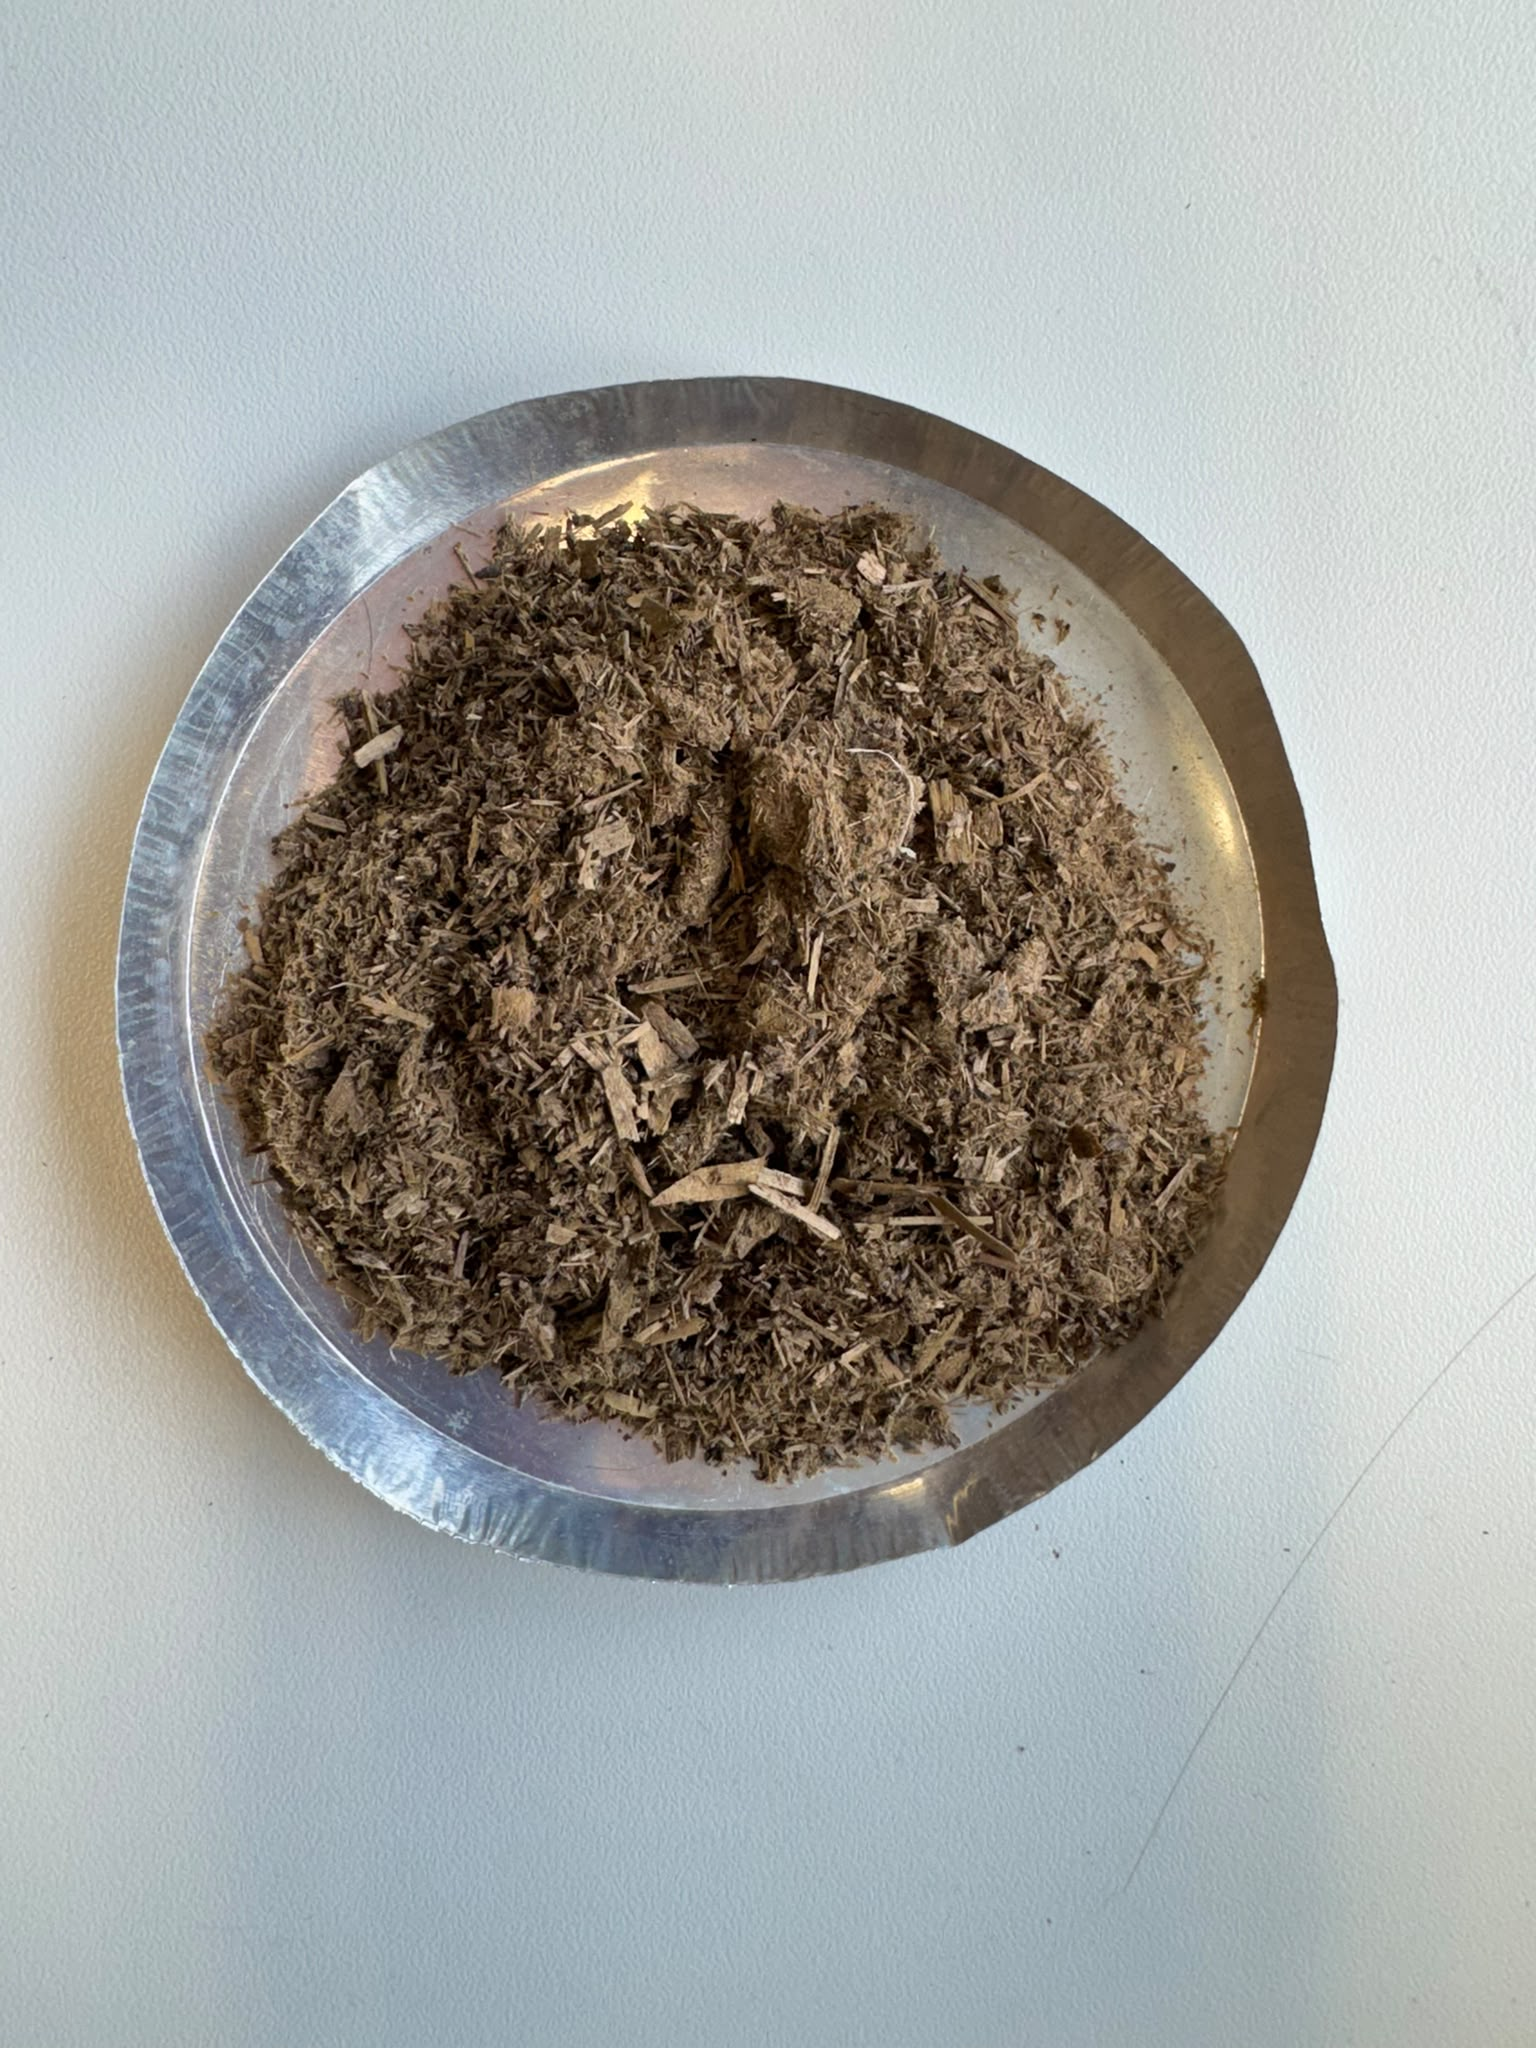
\includegraphics[angle=-90,origin=c]
            {Abbildungen/Algerian Digestate.jpeg}
        }
        \captionof{figure}{
            Algerian digestate obtained from the Centre de Développement
            des Energies Renouvelables (CDER) in Algiers, Algeria.
        }
        \label{fig:3.11}
    \end{minipage}
    \hfill
    \begin{minipage}[t]{0.49\linewidth}
        \centering
        \resizebox{\linewidth}{!}{%
            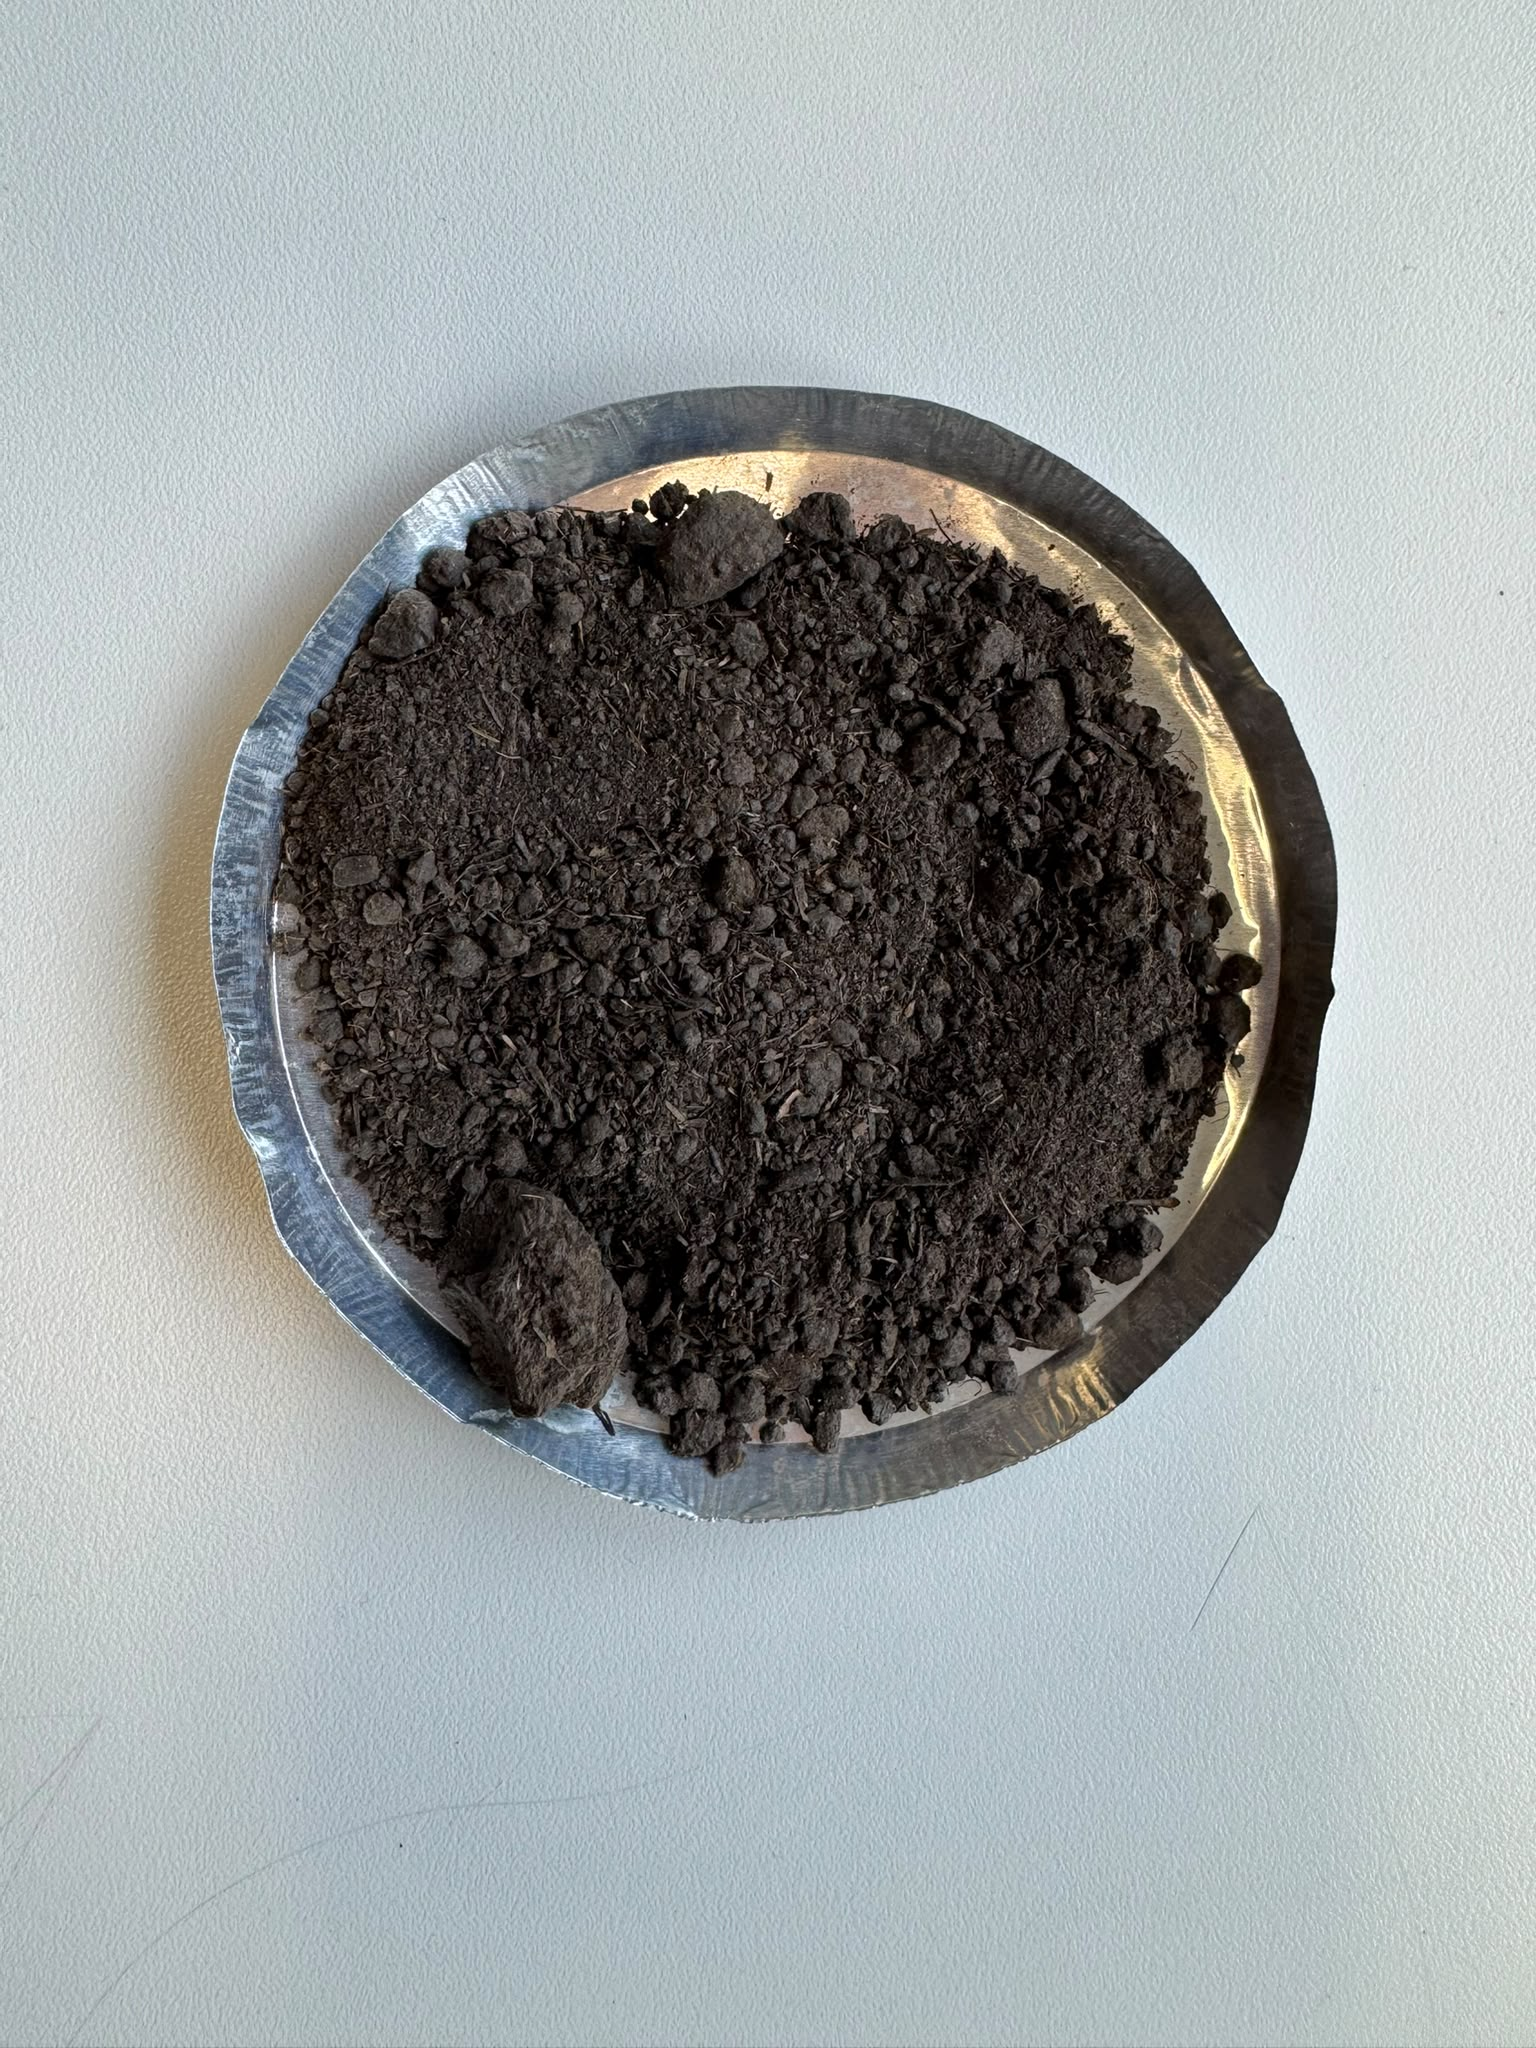
\includegraphics[angle=-90,origin=c]
            {Abbildungen/French Digestate.jpeg}
        }
        \captionof{figure}{
            French digestate obtained from the Centre National de la Recherche
            Scientifique (CNRS-ICARE) in Orléans, France.
        }
        \label{fig:3.12}
    \end{minipage}

\end{figure}

\vspace{0.3em}

The digestate was used in its as-received state for the pyrolysis experiments. After pyrolysis, the resulting biochars were stored in a desiccator to prevent moisture uptake during subsequent storage and handling. A separate drying step using a moisture-analyzing device was applied to digestates and biochars prior to calorific value determination.

\vspace{0.3em}

The reagents and gasses employed in the activation and sulfurization steps were:
\begin{itemize}
    \item Deionized water ($H_2O$) - Activation agent
    \item Argon, $Ar$ with 99,999\% purity - Inert gas for purging prior to activation
    \item Iron(II) sulfide, $FeS$ - sulfide source for $H_2S$ generation
    \item Hydrochloric acid, H$Cl$ - acid reagent for $H_2S$ generation
\end{itemize}

\subsection{Biochar Production via Pyrolysis}
\setresponsible{Surya Salim}
\label{biocharproduction}

Biochar was produced in the laboratory for thermochemical processes in Department 1: Engineering—Energy and Information at the Berlin University of Applied Sciences (HTW Berlin). Biochar was produced from both digestates by slow pyrolysis in an electrically heated laboratory-scale oven. The setup consisted of a programmable temperature-controlled oven and a sealable pyrolysis reactor, as shown in Figure~\ref{fig:3.2.1}. The required heating temperature and duration for the pyrolysis process were set and regulated using the button located right below the chamber. Inside the oven, white refractory ceramic insulation material is used to withstand high temperatures and reduce heat transfer to the outside, ensuring an uniform temperature inside the heating chamber. 

\begin{figure}[H]
    \centering
    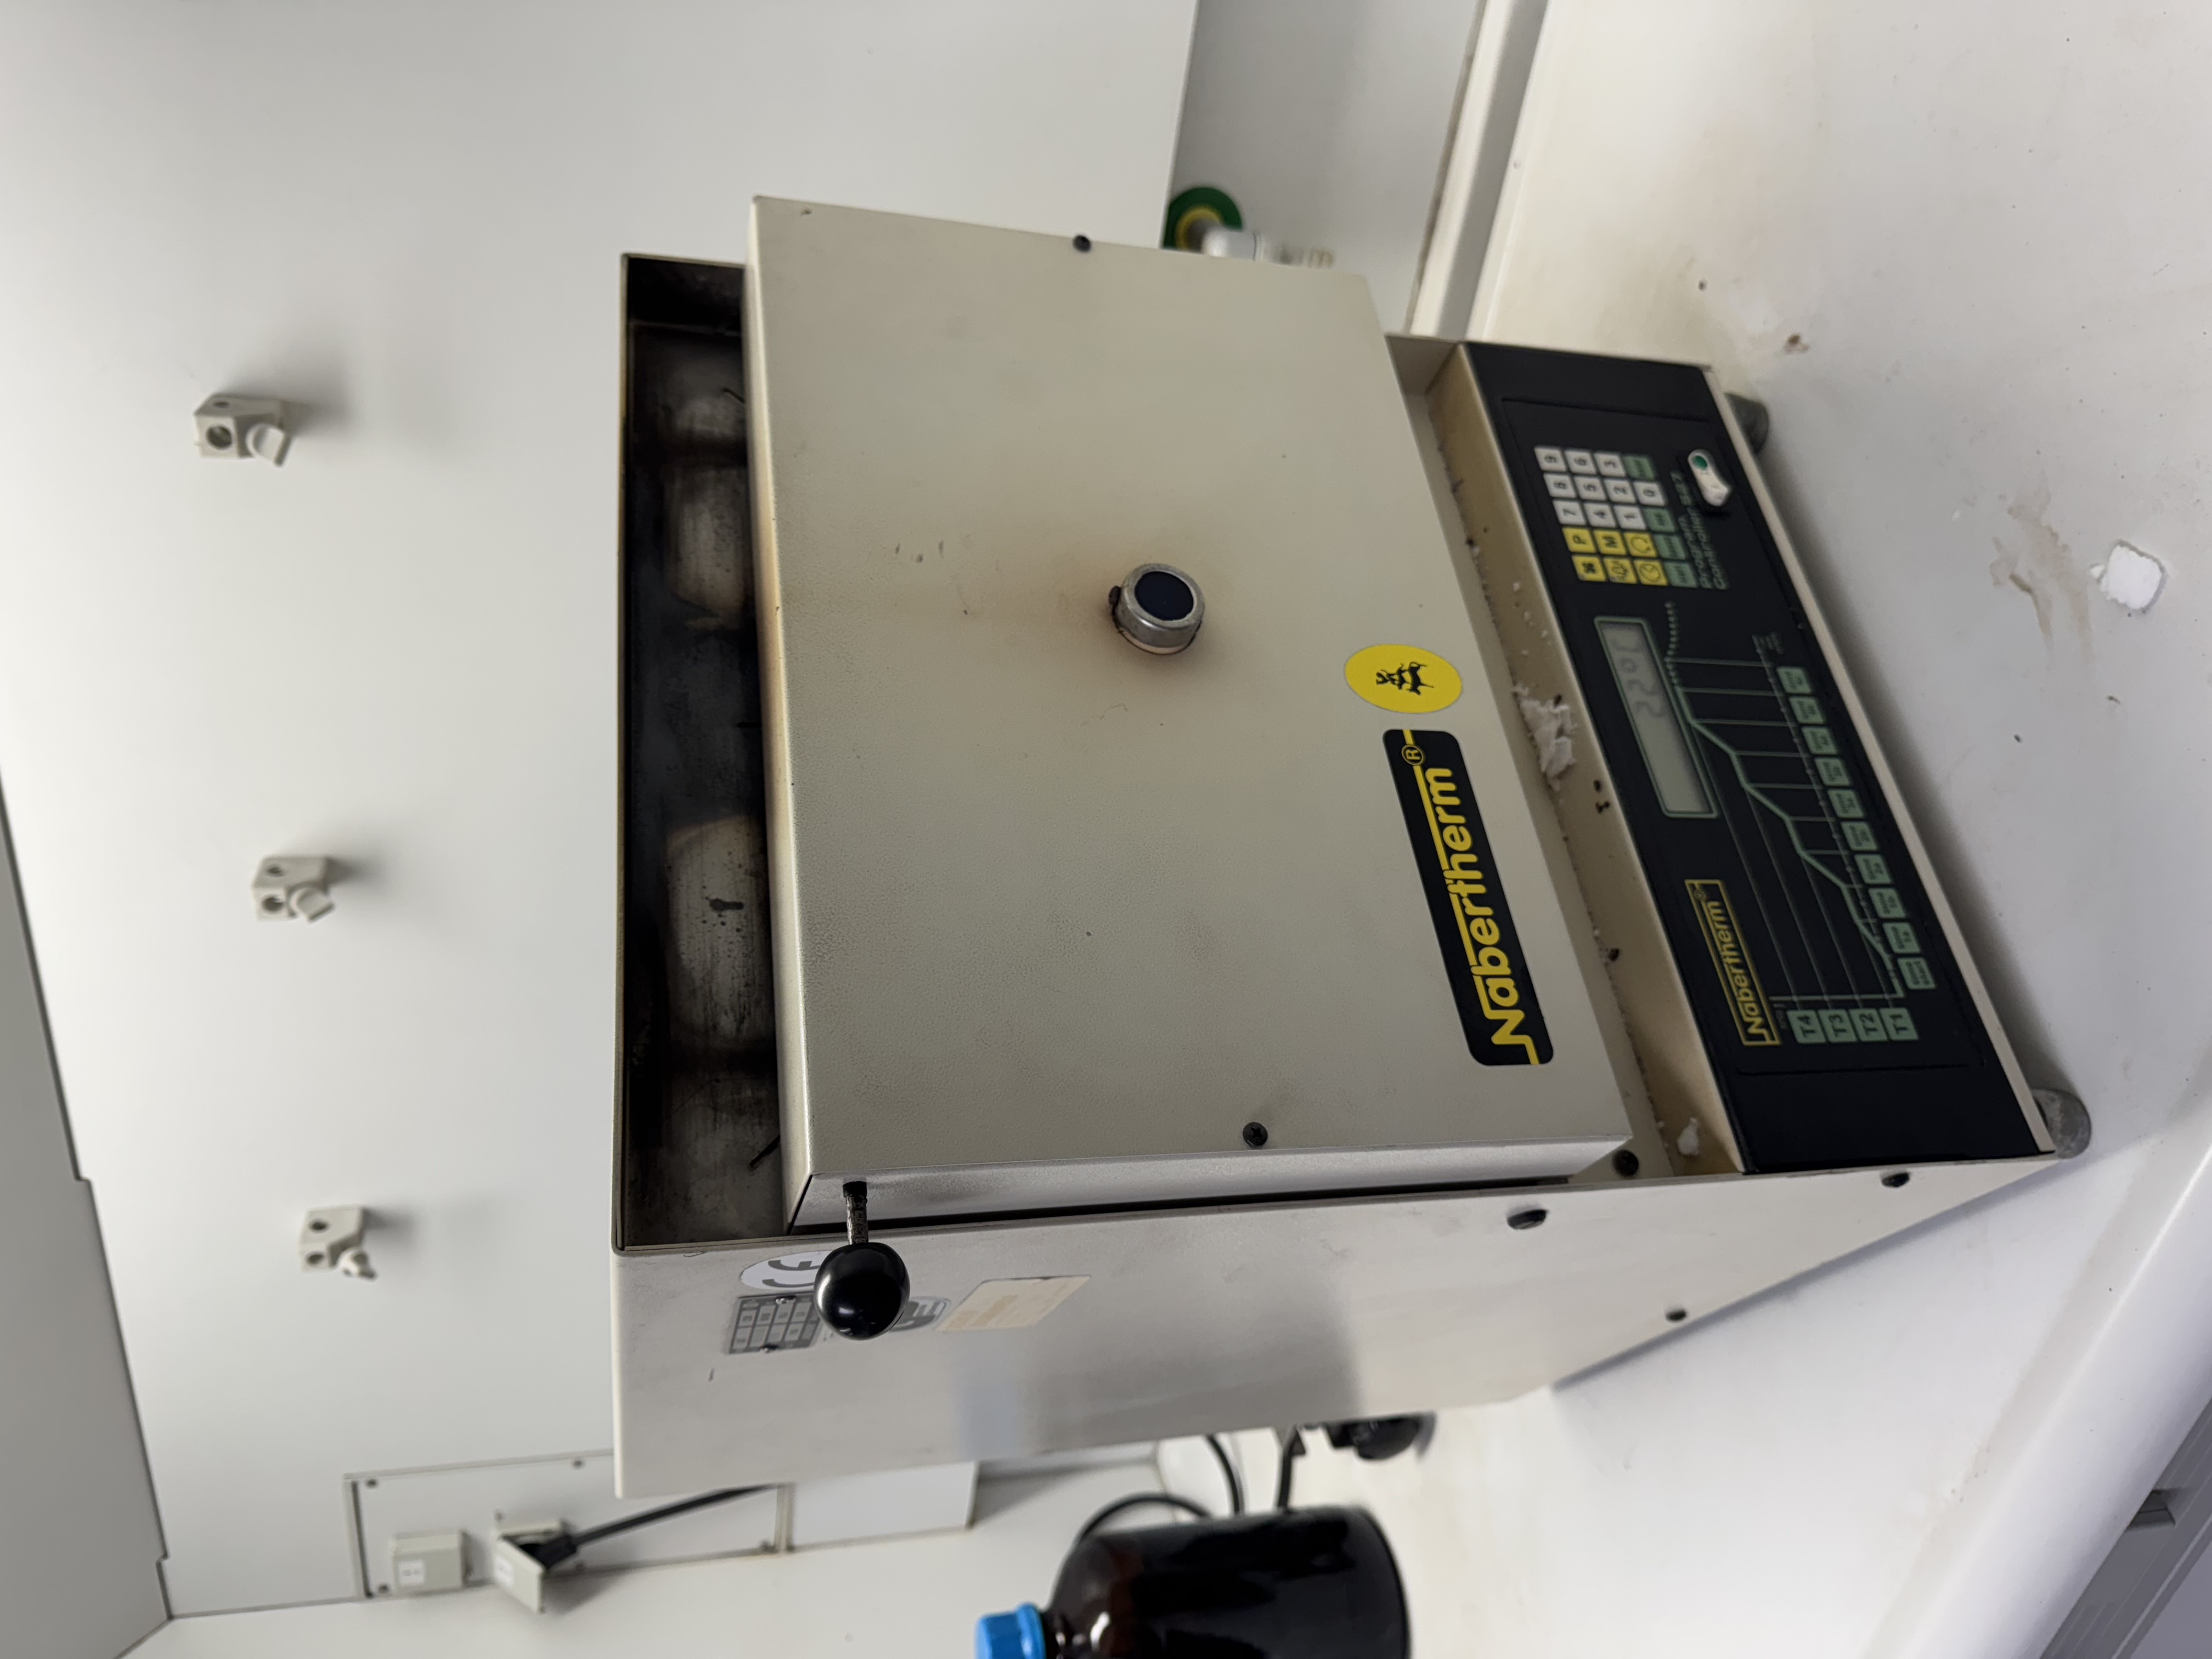
\includegraphics[width=0.8\linewidth, angle=-90]{Abbildungen/Pyrolissi oven.jpeg}
    \caption{Experimental setup for slow pyrolysis}
    \label{fig:3.2.1}
\end{figure}

\vspace{0.3em}

Prior to each run, the reactor was thoroughly cleaned to ensure consistency between experiments, and the gas outlet pipe was inspected to prevent blockages during operation. Due to the limited quantity of the primary substrate (Slaughterhouse digestate, France), pyrolysis was carried out using ceramic crucibles Figure~\ref{fig:3.2.2}, placed inside the reactor rather than by filling the reactor volume directly, as illustrated in Figure~\ref{fig:3.2.3} and \ref{fig:3.2.4} .

\begin{figure}[H]
    \centering
    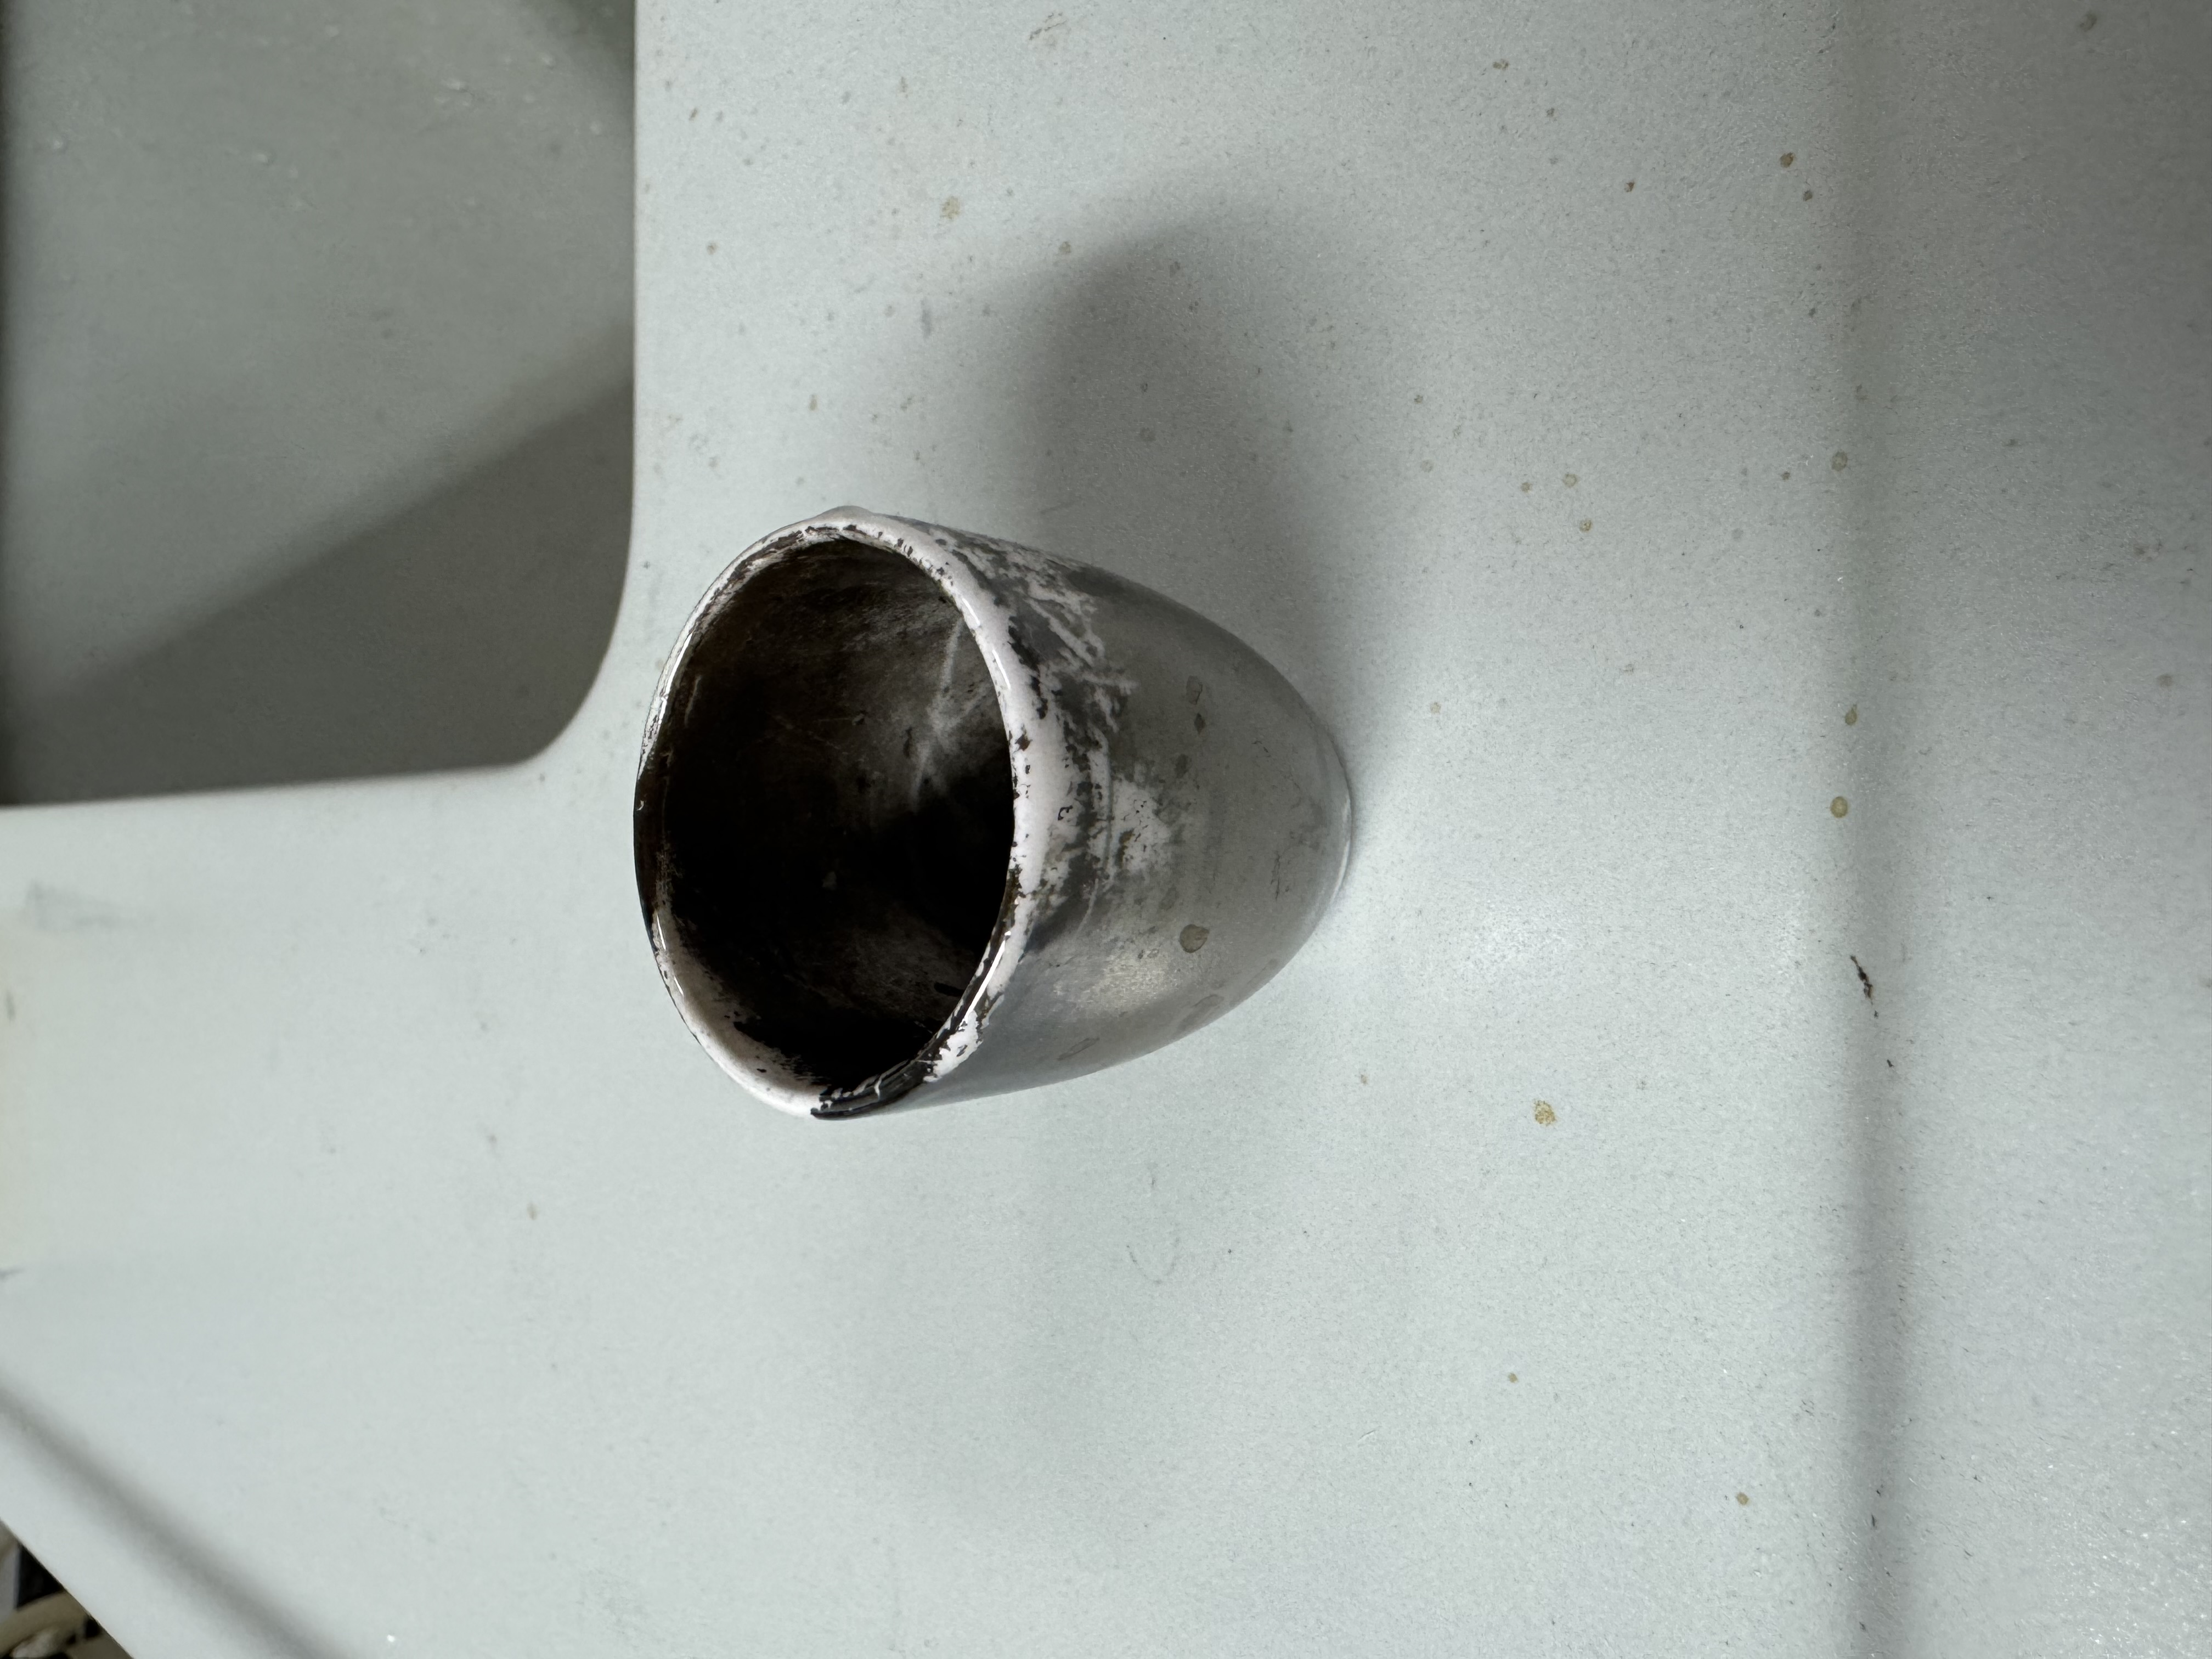
\includegraphics[width=0.7\linewidth, angle=-90]{Abbildungen/Crucible.jpeg}
    \caption{Ceramic crucible}
    \label{fig:3.2.2}
\end{figure}

\begin{figure}[H]
    \centering
    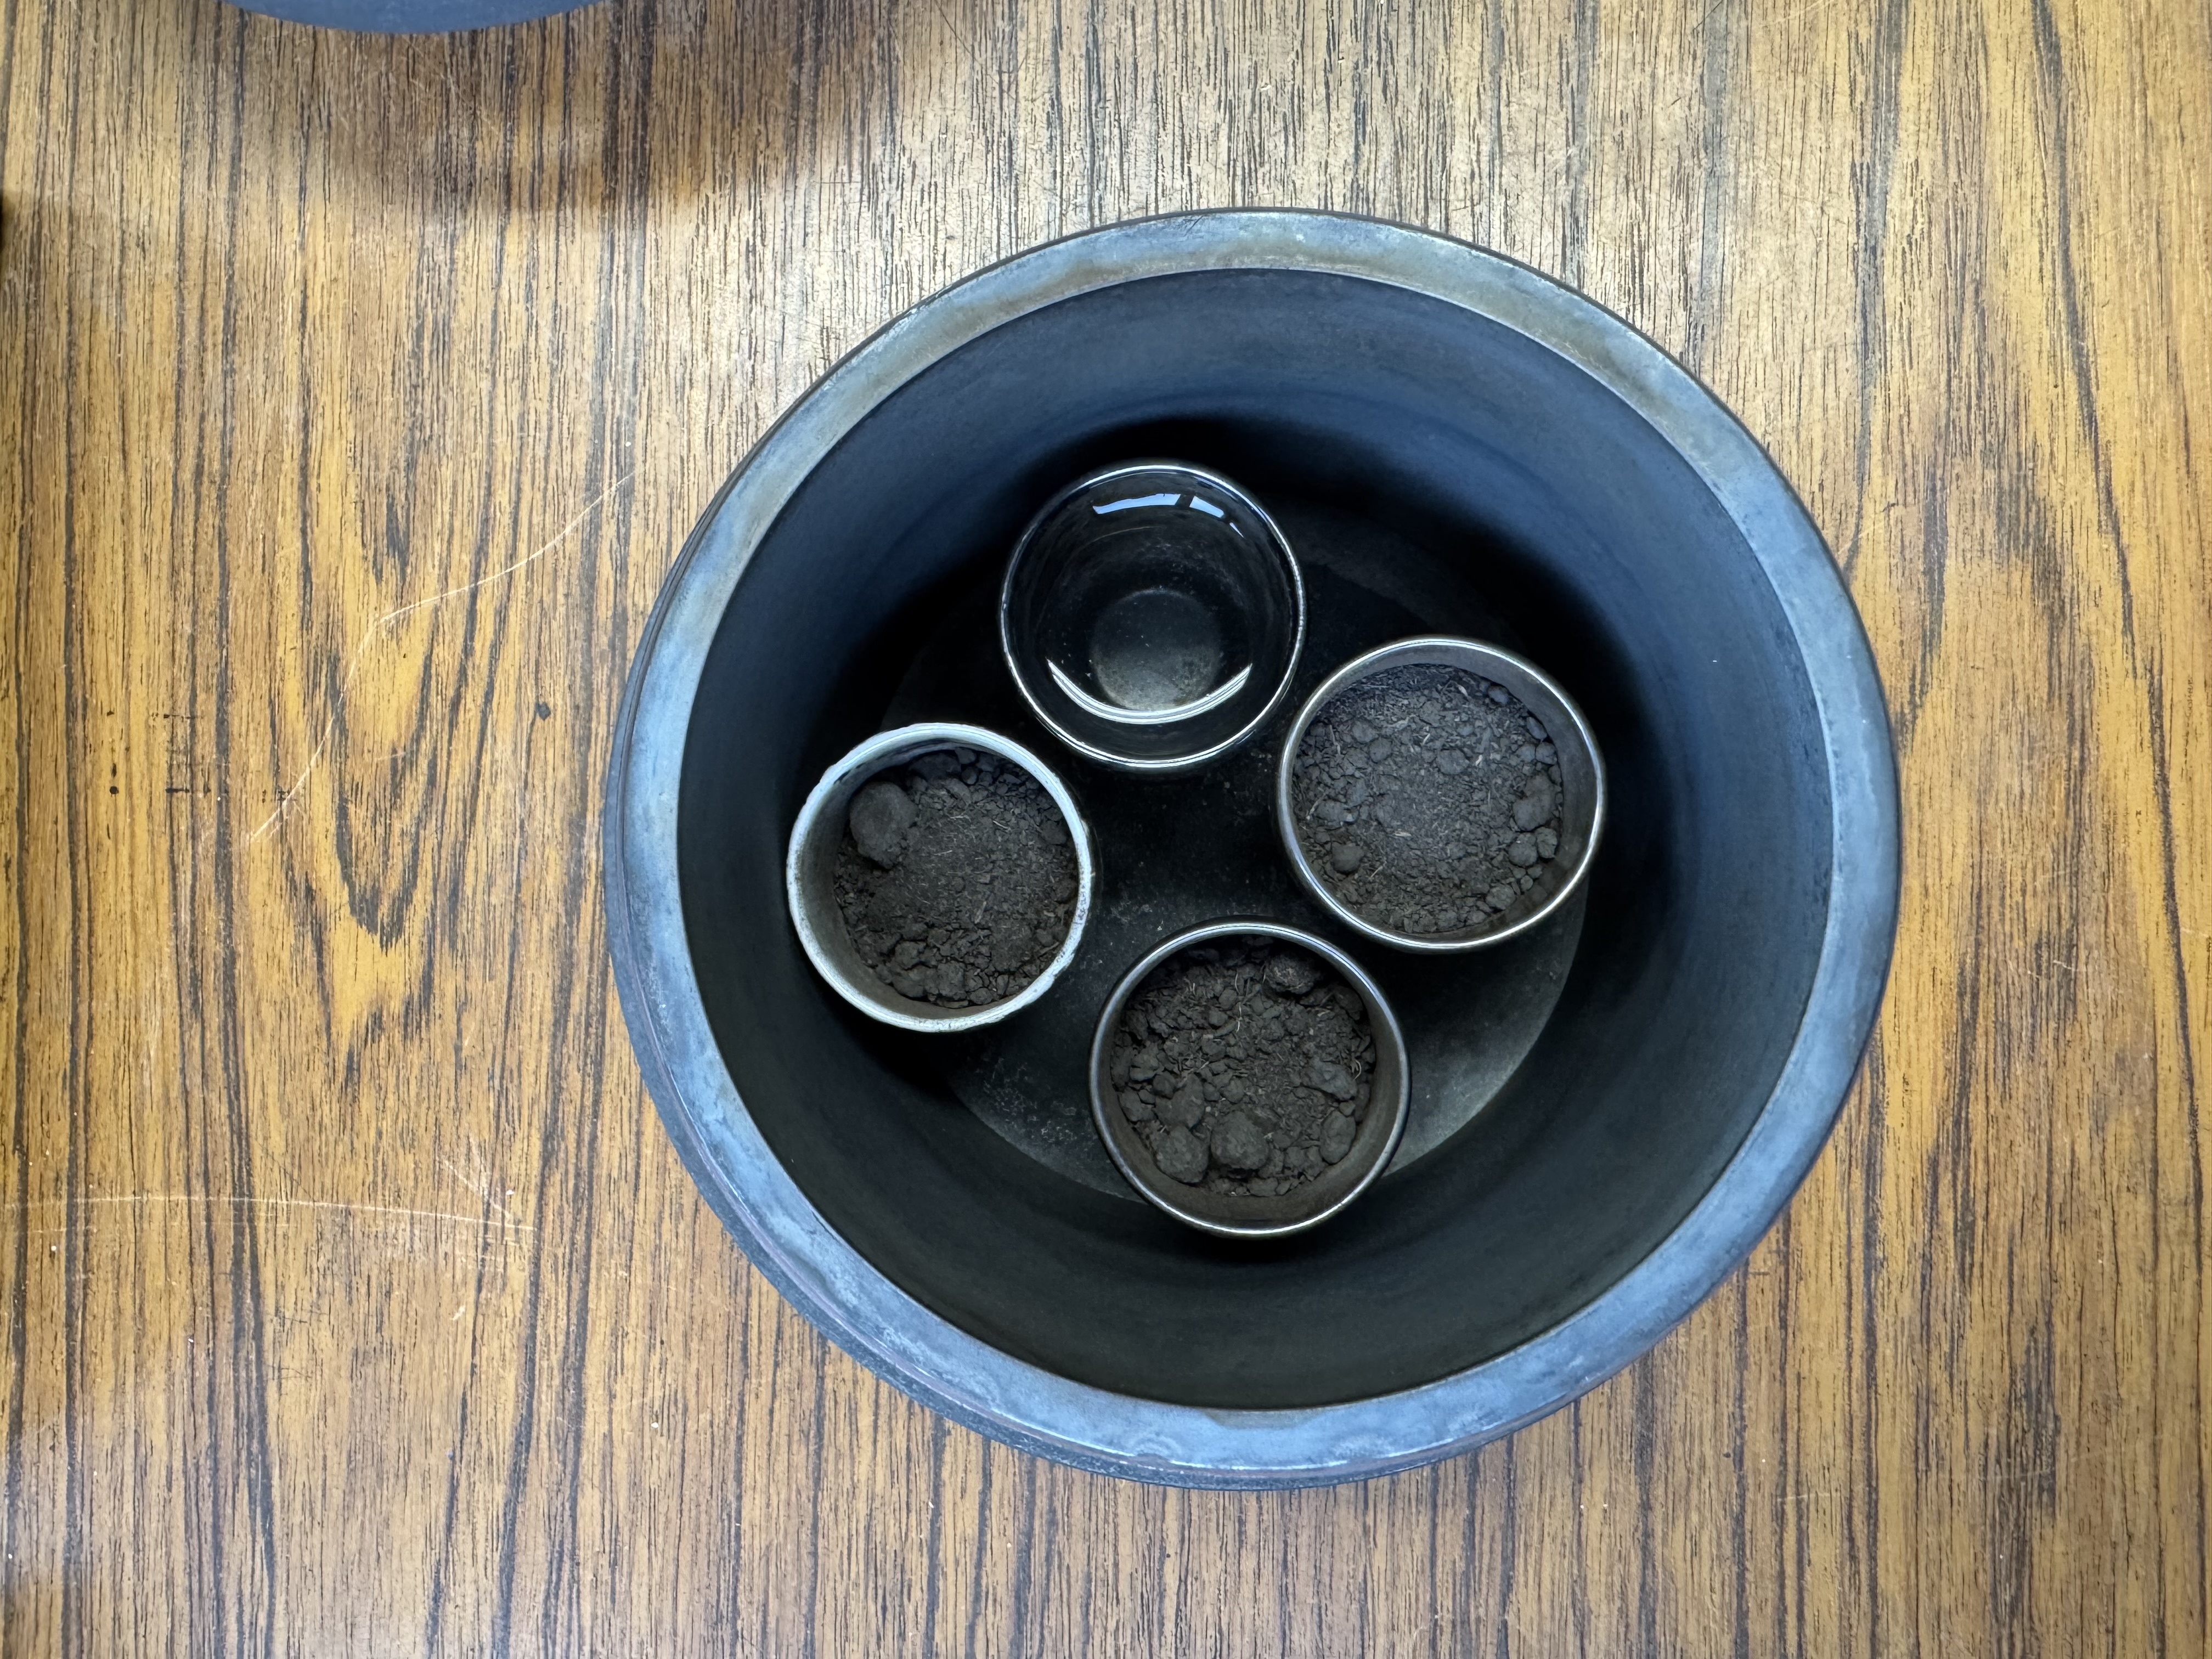
\includegraphics[width=0.8\linewidth]{Abbildungen/IMG_0003 (1).jpeg}
    \caption{The ceramic crucibles filled with biomass and water inside the reactor}
    \label{fig:3.2.3}
\end{figure}

\begin{figure}[H]
    \centering
    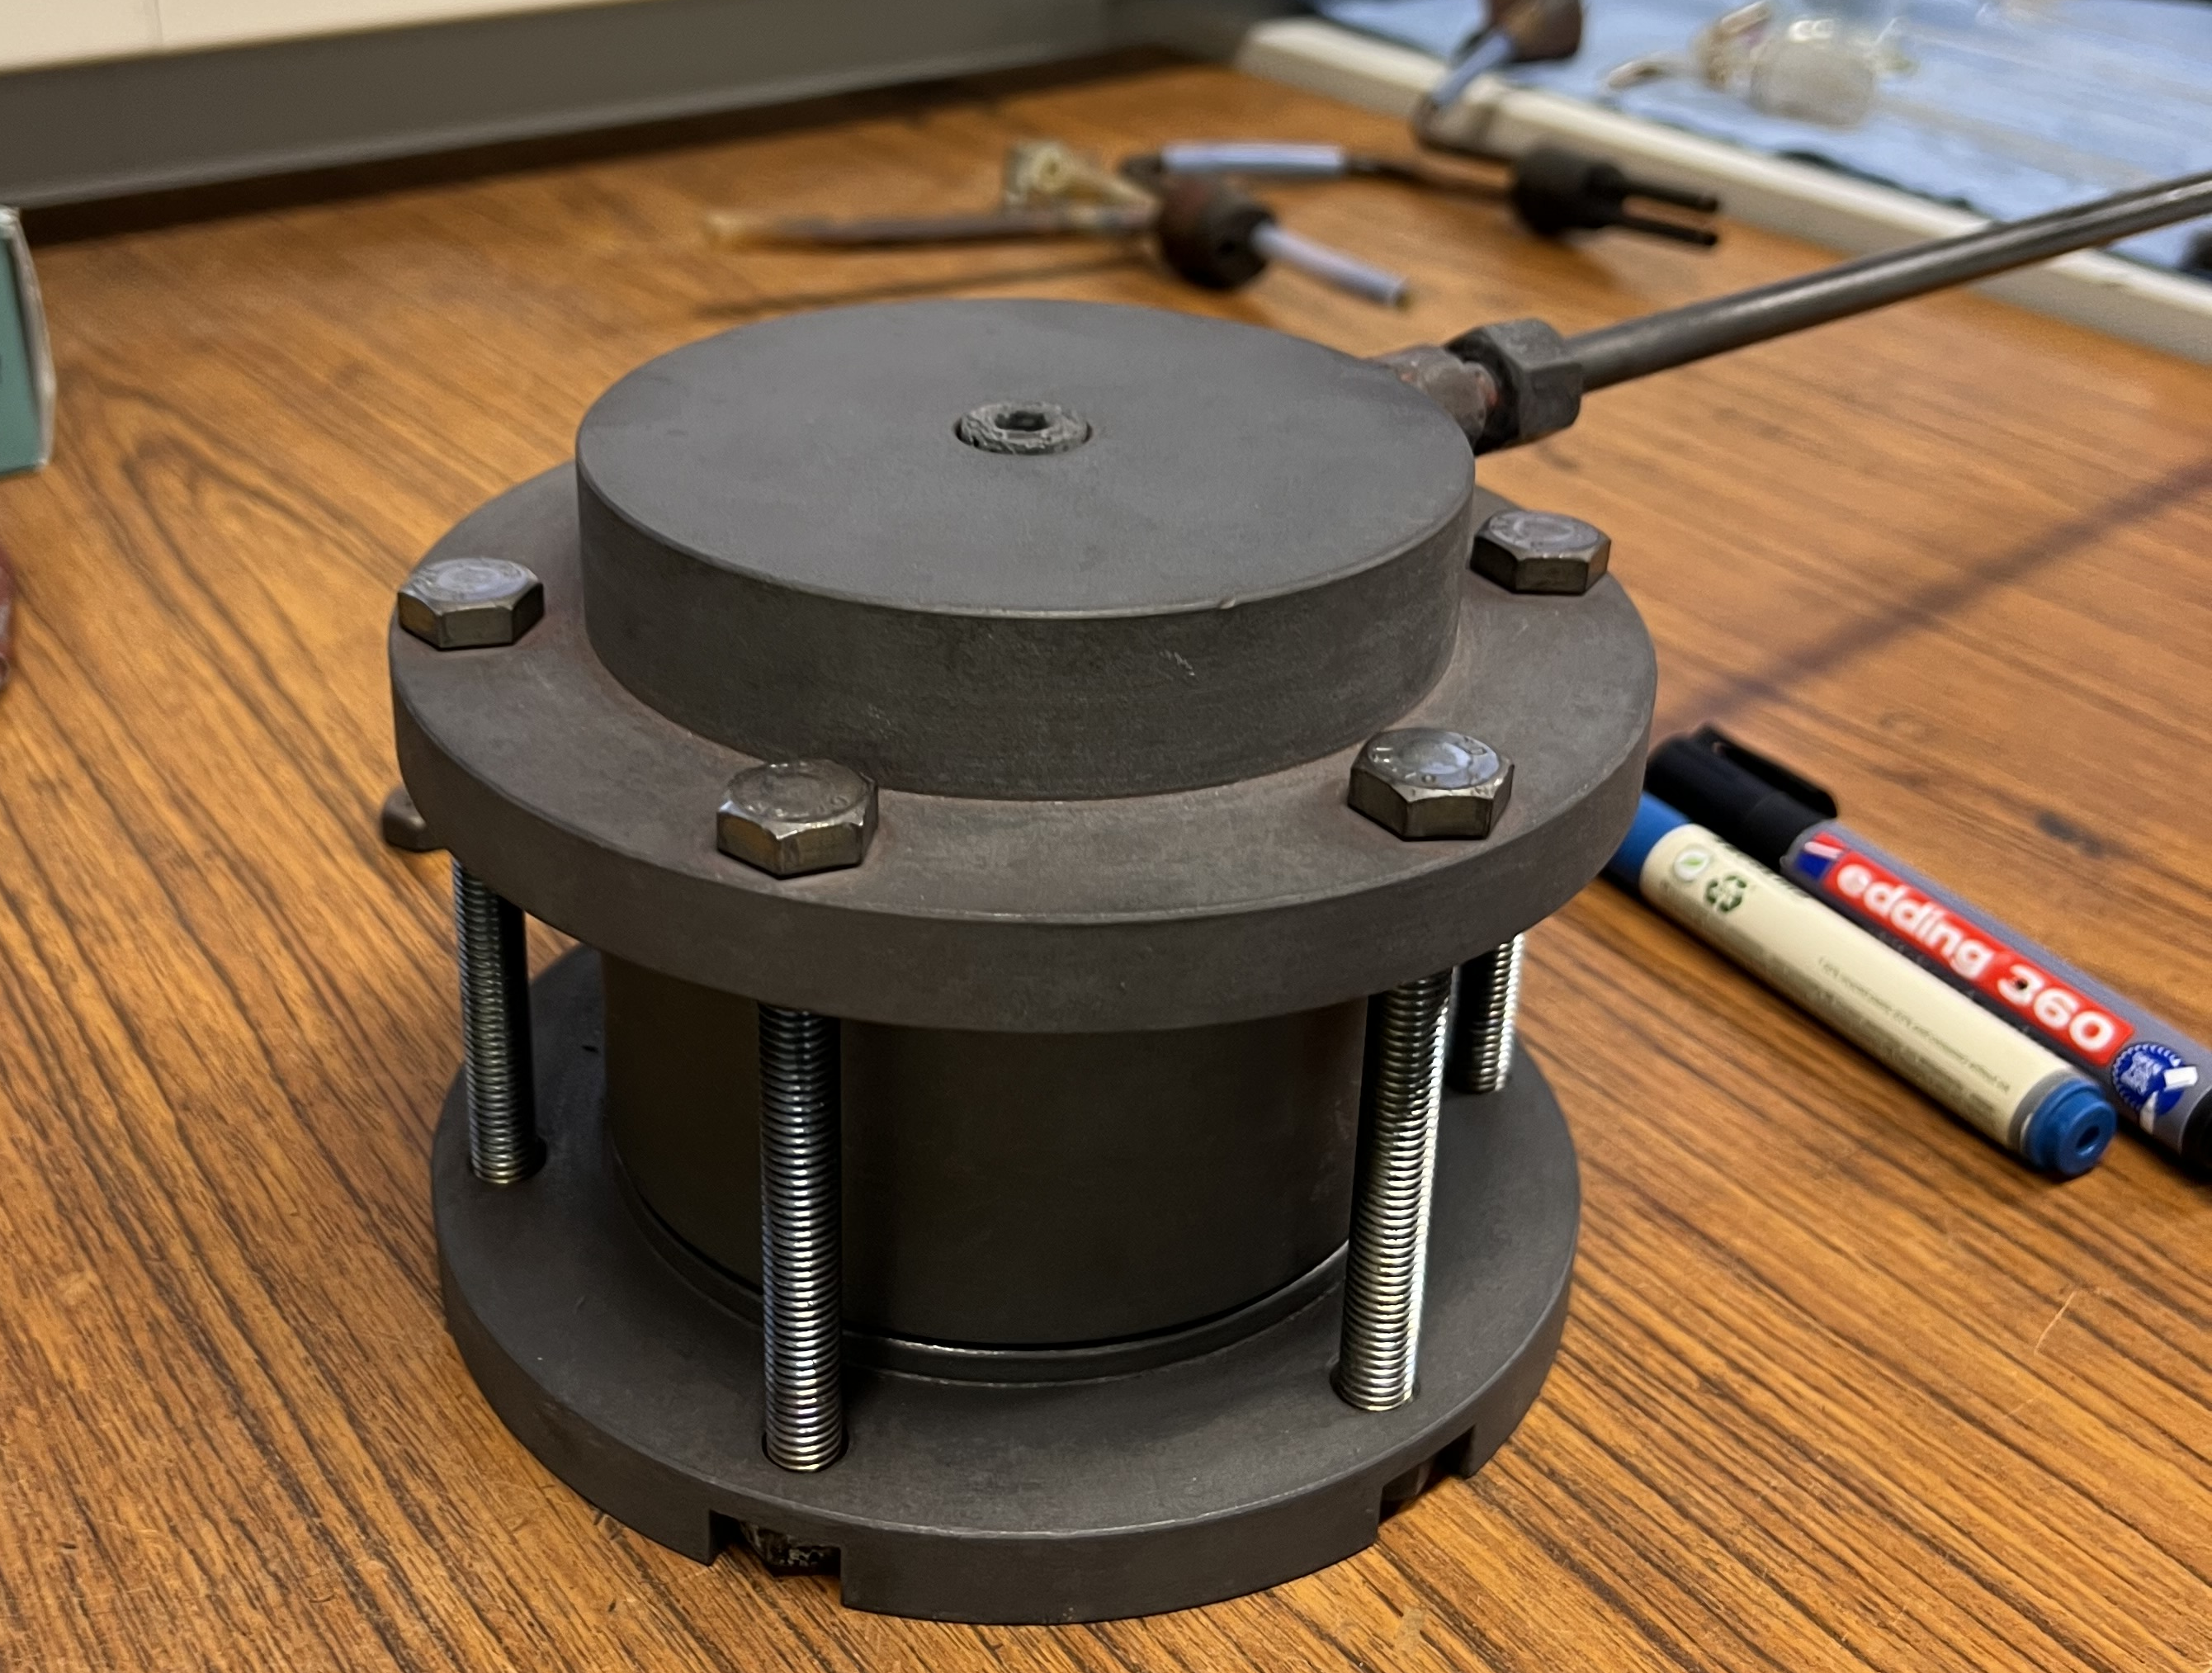
\includegraphics[width=0.8\linewidth]{Abbildungen/Cut-reactor.png}
    \caption{The reactor}
    \label{fig:3.2.4}
\end{figure}

\vspace{0.3em}

For each run, a known mass of digestate (recorded before pyrolysis) was loaded into the crucibles, and an additional crucible containing a defined mass of water was placed alongside the sample crucibles. The water generated water vapor during heating, which helped maintain an oxygen-poor atmosphere within the reactor. 

\vspace{0.8em}

The reactor was first sealed with 6 screws, then placed inside the oven, and heated according to the following programmed conditions:
\begin{itemize}
    \item Heating rate : 10 °C min$^{-1}$
    \item Target temperatures : 400 °C, 500 °C, or 600 °C
    \item Residence time at target temperatures: 1 h
\end{itemize}

Three pyrolysis temperatures were investigated to study the influence of pyrolysis temperature on biochar yield and properties, as discussed in \S~\ref{Influence pyrolysis condition}. After the residence time, the oven was switched off and the reactor was allowed to cool down to relative lower temperature before opening, in order to avoid oxidation of the freshly produced biochar by atmospheric oxygen.

Only the solid product (biochar) was collected and quantified in this study. The condensable bio-oil and non-condensable gas fractions were neither quantified nor characterized. The biochar yield Y was calculated as:
\begin{equation}
    Y = \frac{m_{Biochar}}{m_{Digestate}} \times 100 \%
    \label{eq:biochar yield}
\end{equation}
where $m_{Digestate}$ is the initial mass of digestate loaded into the reactor and $m_{Biochar}$ is the mass of the solid product recovered after pyrolysis. The collected biochars were transferred to plastic containers with name labels on them and stored until further processing in the activation step.

\subsection{\texorpdfstring{H$_2$O}{H2O}-Activation}
\setresponsible{Surya Salim}
\label{subsec:methods-activation}

To develop the porous structure of the biochar produced in \S~\ref{biocharproduction}, a steam activation step was carried out in a separate setup consisting of a horizontal tube furnace (Carbolite) and a reaction tube placed coaxially inside the furnace, as shown in Figures~\ref{fig:3.3.1} and~\ref{fig:3.3.2}. The reaction tube is sealed at both ends by valve-controlled fittings, allowing controlled gas flow during heat-up and full isolation of the reaction volume once the steam phase is initiated. The H$_2$O activation was carried out in the chemistry lab of Department 1: Engineering—Energy and Information, in Building F at the Berlin University of Applied Sciences (HTW Berlin). The activation was carried out exclusively on the biochar produced from the French digestate. The French biochar was designated as the primary substrate for the activation, sulfur loading and characterization steps that follow.
\begin{figure}[ht!]
    \centering
    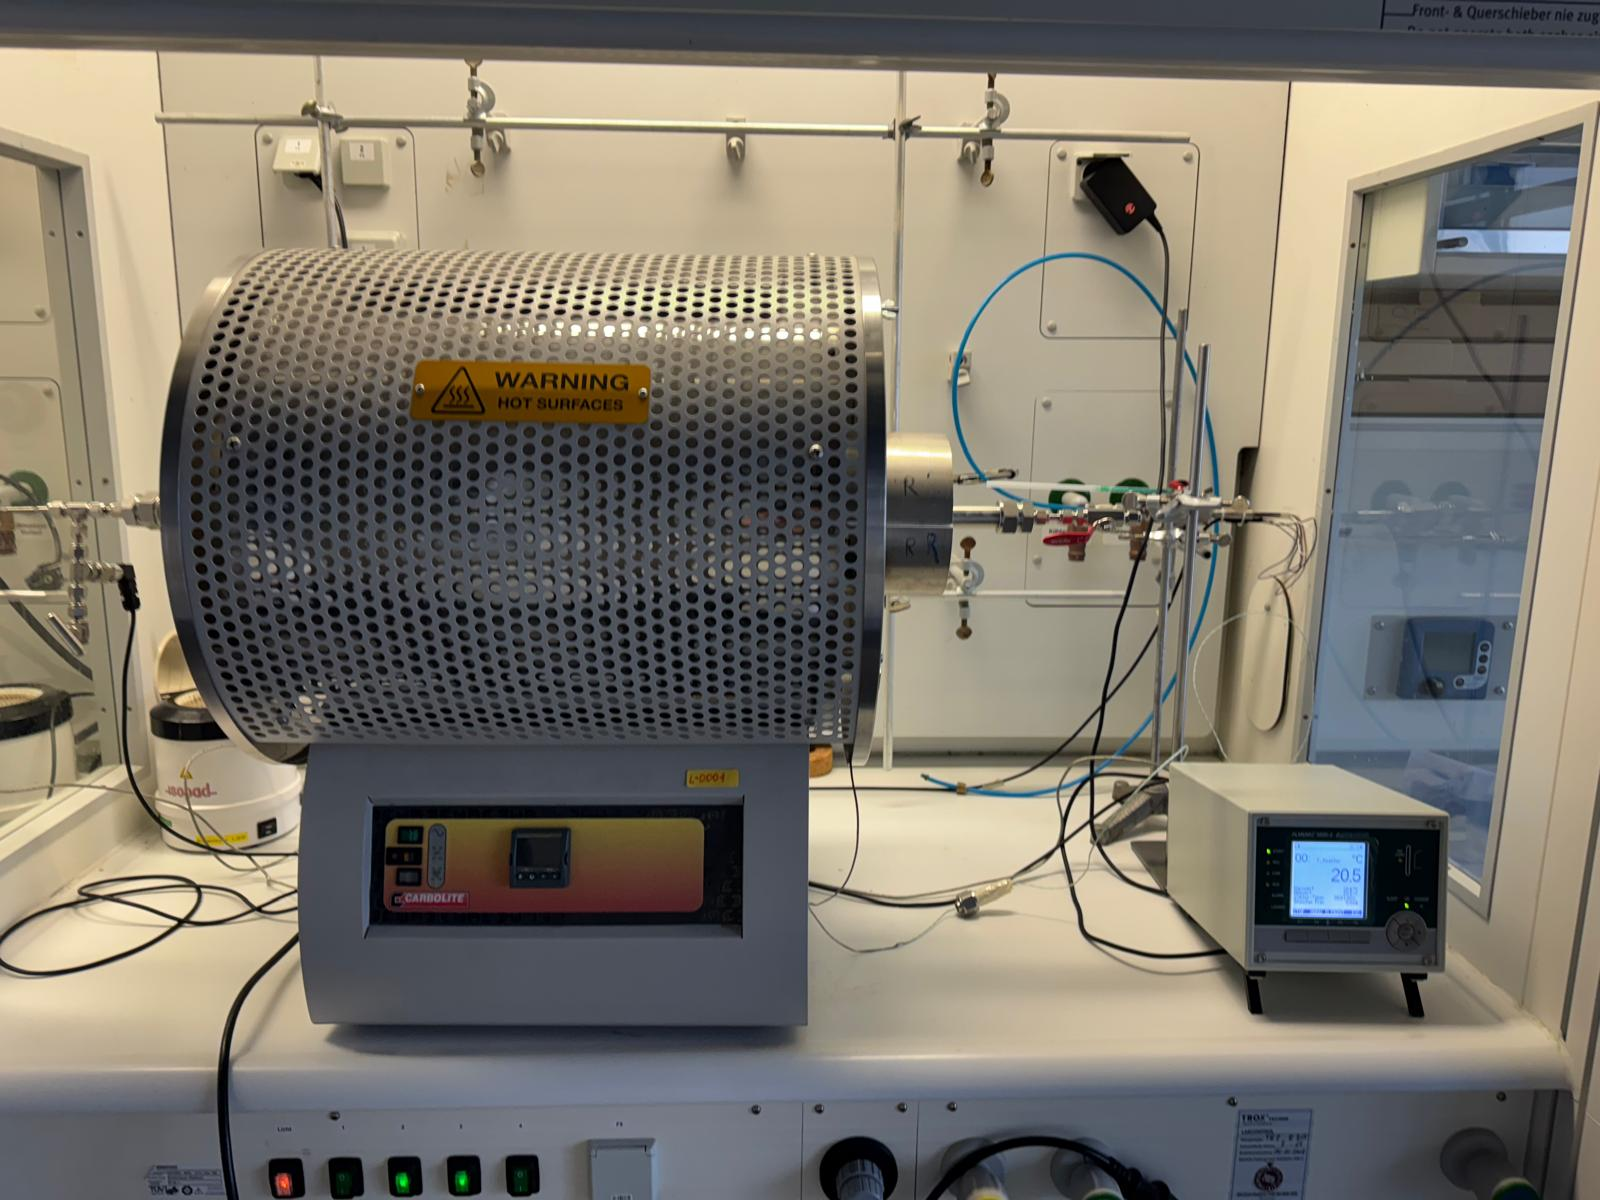
\includegraphics[width=0.8\linewidth]{Abbildungen/Aktivierungsetup.jpeg}
    \caption{Experimental setup for the steam activation of biochar, comprising the tube furnace, reactor tube and temperature controller.}
    \label{fig:3.3.1}
\end{figure}

\begin{figure}[ht!]
    \centering
    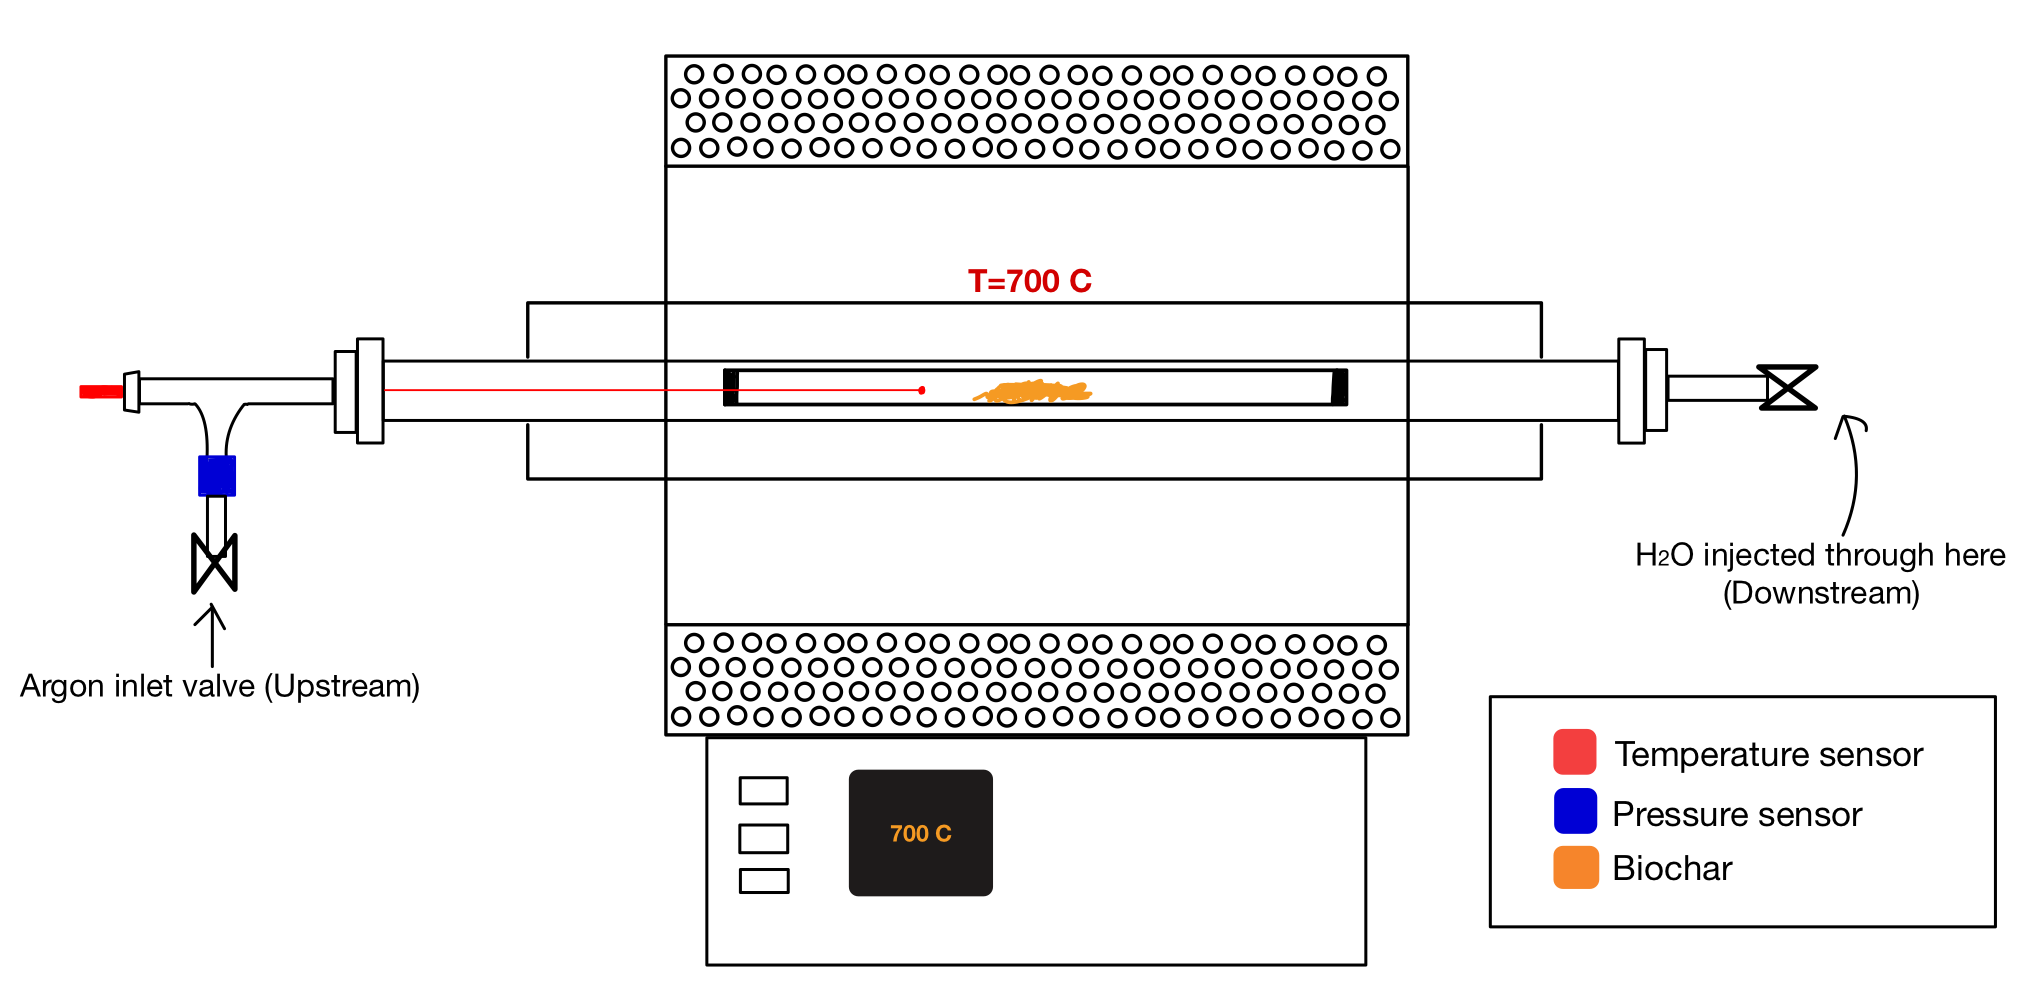
\includegraphics[width=0.8\linewidth]{Abbildungen/Aktivierungsovensketch.png}
    \caption{Schematic cross-section of the steam activation setup, showing the reactor tube within the tube furnace, with the biochar in the heated zone (T = 700 °C).}
    \label{fig:3.3.2}
\end{figure}

\vspace{0.8em}

The amount of water introduced per activation was selected to limit the mass loss of the biochar to below 10\%, in line with the burn-off control objective established in the project work. Although the underlying intent is to limit "carbon" loss, the experimentally accessible quantity in this work is the total mass loss of the biochar before and after activation. The two are equivalent only under the assumption that the steam-carbon reaction :
\begin{equation}
    C \, + H_2O \rightarrow CO \, + H_2
\end{equation}
is the sole mass-removing process. In practice, residual devolatilization of hydrogen- and oxygen-containing functional groups may also contribute to the measured mass loss.

\vspace{0.3em}

For this thesis, the biochar carbon content is assumed approximately 60\% based on preceding project work. Based on this number, a stoichiometric calculation for the respective reaction indicates that, at a uniform tube temperature of 700 °C, only about 0.09 g of water ($\approx$ 0.09 mL at STP) would theoretically be required to gasify 0.06 g of carbon. In practice, however, the temperature is not uniform across the entire tube volume; the central hot zone reaches the set point while the tube extremities remain considerably cooler, so that a non-negligible fraction of the injected water condenses on the cooler tube walls and is not available for reaction with the biochar. The maximum temperature was also set to 700 °C, since the pipe joint could not withstand temperatures exceeding 700 °C.

\vspace{0.3em}

To verify that the 10\% mass-loss target could be met under these non-ideal conditions, a comparative trial was carried out with two water doses applied to 1 g biochar from each pyrolysis temperature : 0.1 mL (close to the theoretical minimum) and 0.5 mL (a fivefold excess intended to compensate for steam losses to condensation). The resulting losses were essentially identical for the 500 °C  biochars (see table~\ref{tab:activation-full}). On the wet basis, both doses sat near or below 10\%, while moisture-corrected losses ran 10-22\%. 

\vspace{0.3em}

On this basis, the 0.5 mL of water per 1 g of biochar dose was adopted as the standard activation condition. All activated biochars used thereafter for the elemental and surface analyzes described in \S~\ref{sec: Analyticalmethods} were produced under this condition. The 0.1 mL dose was retained only as a comparative reference for the activation study. The same dose ratio was additionally checked at twice the scale. In runs 10--12 (Table~\ref{tab:activation-full}), 2\,g of biochar was activated with 1.0\,mL of water, and the
moisture-corrected mass losses followed the same descending order with pyrolysis temperature as
the corresponding 1\,g runs.

\subsubsection*{Activation procedure}
\begin{enumerate}
    \item \textbf{Inert purging and heat-up} \newline
    Argon was introduced from the upstream end (or left side of Figure \ref{fig:3.3.2}) of the tube and allowed to exit through the other end of the tube valve. The argon flow was kept deliberately low to maintain an inert atmosphere without blowing off the biochar. Simultaneously, the furnace was switched on and programmed to reach a set point of 700 °C at a heating rate of 10 K min$^{-1}$.
    \item \textbf{Transition to steam atmosphere} \newline
    Argon pushing was continued until the downstream end (or right side of Figure \ref{fig:3.3.2}) of the tube reached a temperature above 100 °C. This ensures that injected liquid water would flash to vapor rather than condense at the injection point. At this point, before injection, the argon flow was stopped and both valves of the tube were closed.
    \item \textbf{Water injection and sealed activation} \newline
    A single dose of 0.5 mL of deionized water was manually injected through the downstream valve using a syringe. The downstream valve was closed immediately after injection, isolating the reaction tube from the surrounding atmosphere. Under these closed-tube conditions, the injected water flashed to steam in the hot central region and reacted with the biochar over the activation period. The 1 h activation period was timed from the moment of water injection. Some condensation of steam in the cooler tube extremities is expected. Consequently, not all of the injected water vapor is assumed to participate in the steam-carbon reaction.
    \item \textbf{Cool-down} \newline
    After the 1 h hold, the furnace was switched off and the system was allowed to cool to ambient temperature overnight.

    After cooling, the activated biochar was recovered from the reactor tube and weighed. The activation mass loss was calculated on a wet basis as:
    \begin{equation}
        \Delta m_{active,wet}=\frac{m_{before}-m_{after,wet}}{m_{before}} \times 100\%
    \end{equation}
    Because water was introduced during activation by spraying, this initial post-activation mass still contained moisture that had to be separated from the actual mass change caused by activation. Residual moisture was determined gravimetrically using another halogen moisture analyzer (PCE-MA series, PCE Instruments GmbH, Germany) operating on the loss-on-drying (LOD) principle. The instrument heats the sample by means of halogen lamps and calculates moisture content from the mass difference before and after drying; a drying temperature of 190 °C was used. As the analyzer required a minimum sample mass to produce a stable reading, two inert metal rings (combined mass $m_{Nutrings}$=20.74 g) were placed in the sample pan together with each biochar sample to meet this threshold. The rings were first dried so they contributed no moisture of their own, meaning the entire water mass detected during drying originated from the biochar.
    
    Because the analyzer reports moisture as a fraction of the total mass in the chamber, the reported value $w_{dryer}$ refers to the combined mass of biochar and metal rings rather than to the biochar alone. To get the true biochar moisture content:
    \begin{equation}
        w_{bio}=\frac{w_{dryer}\times(m_{after,wet}+m_{Nutrings})}{m_{after,wet}}
    \end{equation}
where $m_{after,wet}$ is the post-activation mass of the biochar prior to drying. After this  the value of $m_{after,dry}$ could be known thus also the total mass loss both from activation and also from the moisture which can be described as :
\begin{equation}
    \Delta m_{loss}=\frac{m_{before}-m_{after,dry}}{m_{before}} \times 100\%
\end{equation}
    \begin{equation}
        \Delta m_{loss}=\frac{m_{before}-(m_{after,wet}(1-w_{bio}))}{m_{before}} \times 100\%
    \end{equation}
    where $m_{before}$ is the mass of biochar loaded into the tube and $m_{after,dry}$ is the post-activation mass after drying. The activated biochars were stored in a glass container until further use in the sulphurization step.
\end{enumerate}

\subsection{Sulfur Loading}
\label{subsec:methods-sulfur-loading}
\setresponsible{Regen Wijaya}

The sulfur loading was carried out in the same chemistry laboratory where the H$_2$O activation took place. The sulfur loading process is carried out exclusively for activated biochar produced from French digestates. The process was conducted in the same chemistry laboratory room, using a simple laboratory-scale setup that resembles the principal process of biogas desulfurization. The setup consists of a magnetic stirrer, a reaction flask equipped with a dropping funnel, glass tubes, and connector tube (Figure \ref{fig:Schwsetup}), all of which are placed in an enclosed chamber equipped with a suction function.

\vspace{0.3em}

\begin{figure}[ht!]
  \centering
  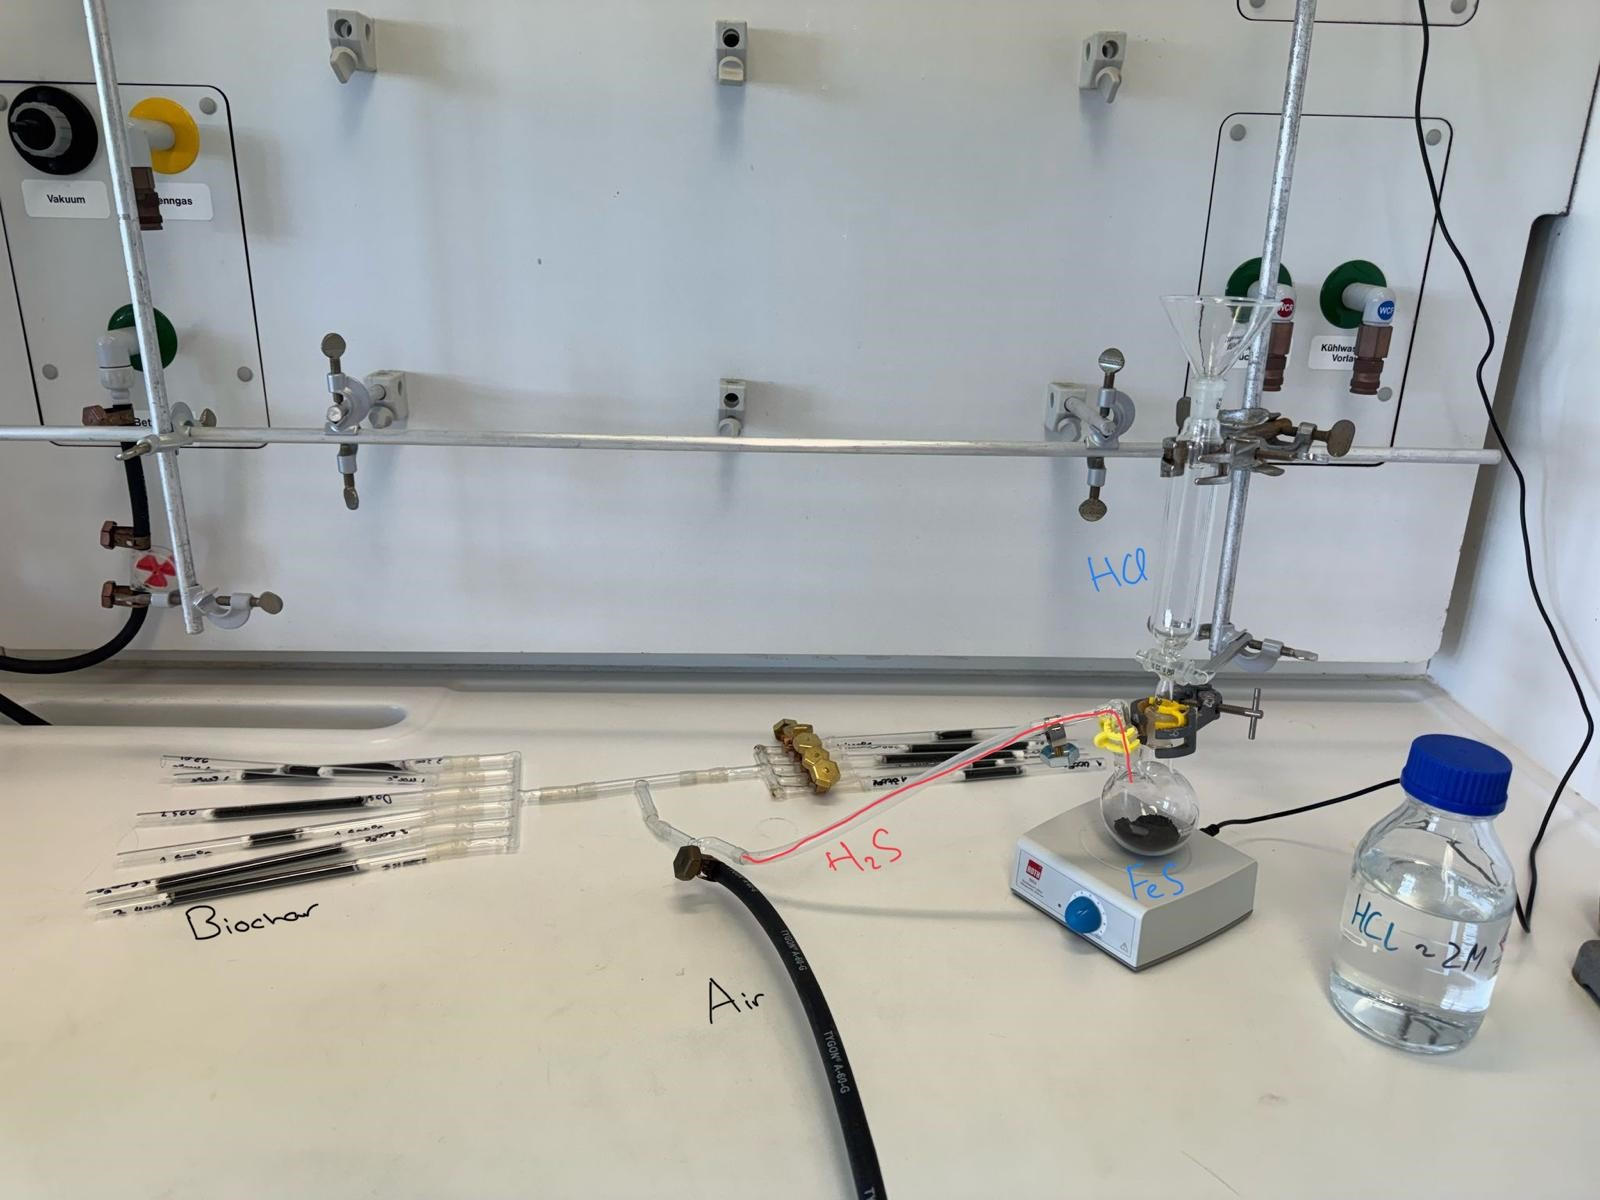
\includegraphics[width=0.8\linewidth]{Abbildungen/Schwefelbeladung Setup .jpg}
  \caption{The setup to load sulfur on the surface of biochar}
  \label{fig:Schwsetup}
\end{figure}

Firstly, the activated biochars were placed inside glass tubes that were open at both ends and plugged at both ends with cotton wool to keep the samples in place while allowing the gaseous flow of hydrogen sulfide to pass through without causing blockage. Each tube was connected to a Y-connector, which was linked to an air source and a reaction flask. 

\vspace{0.3em}

In the reaction flask, pulverized iron sulfide was placed and reacted gradually with droplets of hydrochloric acid from the funnel until the formation and release of hydrogen sulfide gas occurred, which can be characterized by the presence of continuous bubbling in the solution. The generated gaseous hydrogen sulfide was then directed to a Y-connector, where the $H_2S$ stream was introduced to the air stream. The resulting gaseous mixture then flowed through the activated biochars via each glass tube, where partial oxidation of H$_2$S to elemental sulfur was intended to occur on the biochar surface. The whole process lasted for approximately 30 minutes, allowing as much sulfur as possible to be absorbed on the surface of the biochar. Once the entire process was complete, the experimental setup was left undisturbed until the next day. The biochars were then dried and weighed.

\vspace{0.3em}

The sulfur adsorption capacity is represented by the quantity of sulfur adsorbed on the surface of biochar. It is evaluated gravimetrically by dividing the mass increase, which is the difference between the mass before and after the sulfur loading and drying process, by the initial mass of the biochar. It is then defined in milligrams per gram of biochar, as shown in Equation~\ref{Equation sulfur loading}.

\begin{equation}
q_s = \frac{m_{\mathrm{after,s}} - m_{\mathrm{before,s}}}{m_{\mathrm{before,s}}} \times 1000
\label{Equation sulfur loading}
\end{equation}

\subsection{Analytical Methods}
\label{sec: Analyticalmethods}
The analytical methods described in this section were applied to the raw digestate as well as to the biochars obtained after pyrolysis, $H_2O$ activation, and sulfurization, in order to evaluate the effect of each processing step on the resulting material properties.


\subsubsection{Calorific Value Determination (Bomb Calorimetry)}
\label{subsubsec:methods-calorimetry}
The higher heating value (HHV) of the raw digestate and the biochars was determined using an isoperibolic bomb calorimeter (IKA C 200, IKA-Werke GmbH \& Co. KG; Figure~\ref{fig:bombcalori}) following the principle described in \S~\ref{subsubsec:HHV}. The instrument was calibrated at the beginning of each measurement campaign using certified benzoic acid pellets, which served as the reference material for determining the effective heat capacity $\varepsilon$ of the calorimeter system.

\begin{figure}[htbp]
  \centering
  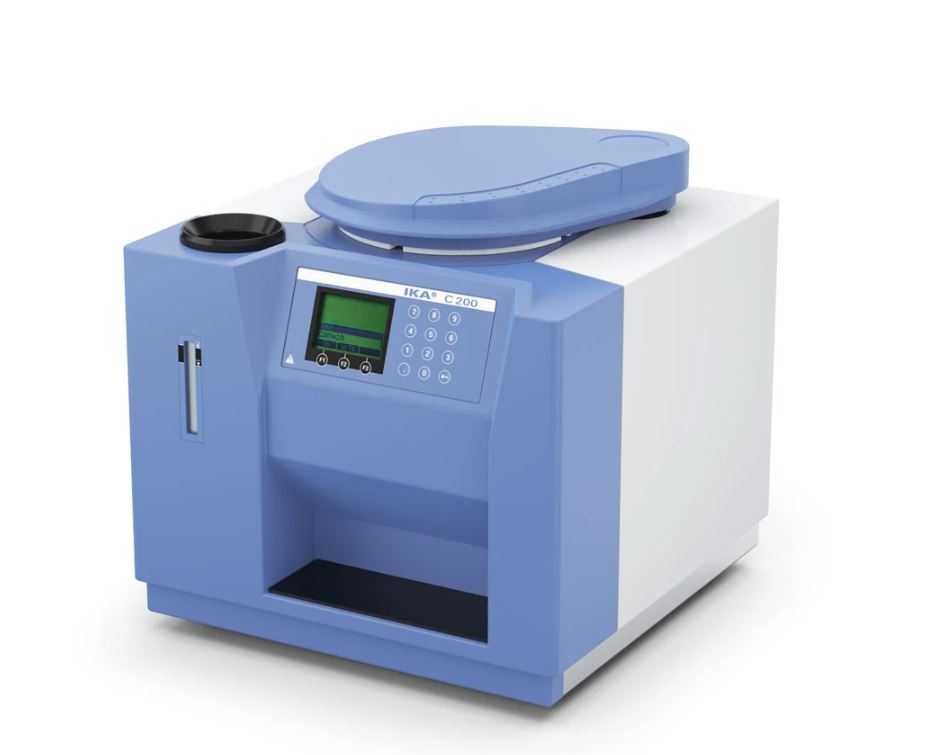
\includegraphics[width=0.88\linewidth]{Abbildungen/Kalorimeter.JPG}
  \caption{IKA calorimeter C 200}
  \label{fig:bombcalori}
\end{figure}

\vspace{0.3em}

Prior to each measurement, biochars were dried to remove residual moisture using a halogen moisture analyzer (PCE-MB 210C, Figure~\ref{fig:moisture_analyzer}) operated at 100°C until constant mass was reached, with the device evaluating dryness via a switch-off criterion of 10 s without further mass change. The dried biochars were transferred to a desiccator and kept there until measurement to prevent the re-uptake of atmospheric moisture. The moisture content displayed by the device was used solely as a process control to confirm that the biochar had reached a dry state and was not to be reported as an independent result.

\begin{figure}[H]
    \centering
    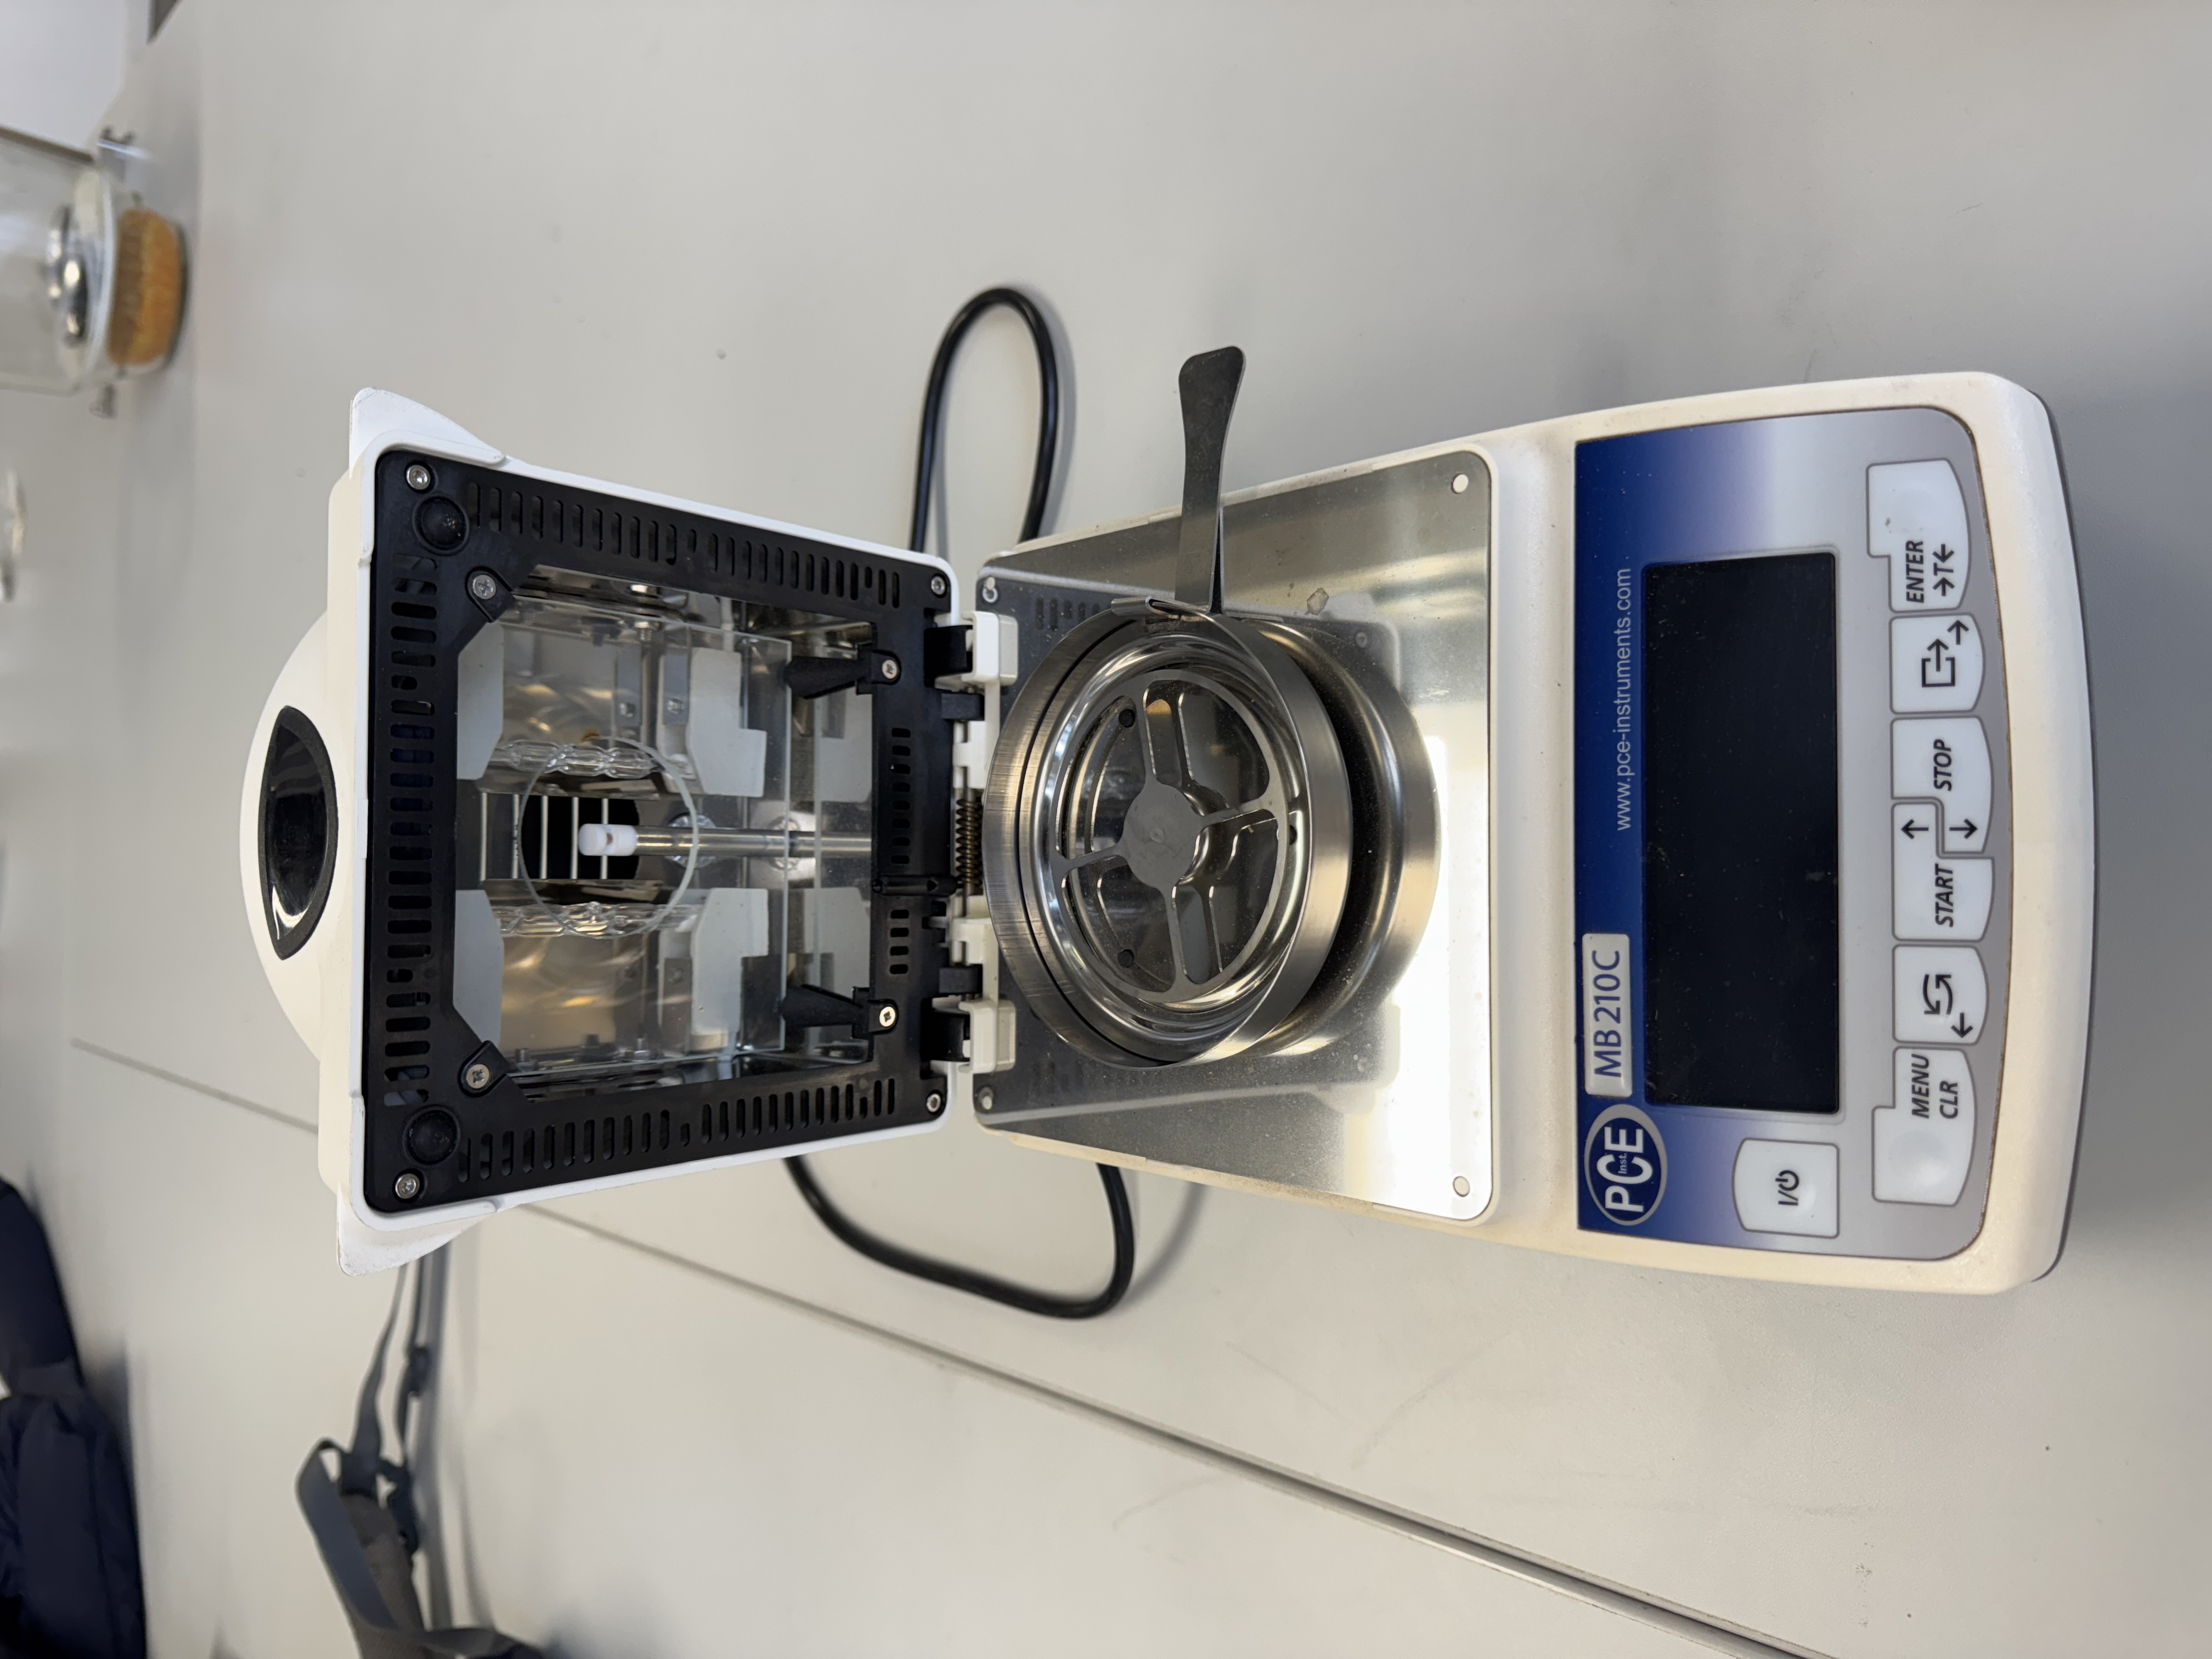
\includegraphics[
        angle=-90,
        origin=c,
        height=0.40\textheight,
        keepaspectratio
    ]{Abbildungen/moisture analyzer.jpeg}
    \caption{Halogen moisture analyzer PCE-MB 210C}
    \label{fig:moisture_analyzer}
\end{figure}

\vspace{0.3em}

For each measurement, approximately 1.0 g of dried biochar was placed in the crucible and then inserted into the bomb. The bomb was sealed and pressurized with pure oxygen to ensure complete combustion. Combustion was initiated electrically via an ignition wire in contact with a thread, which was also in contact with and buried within the biochar. The temperature rise of the surrounding water bath was recorded by the instrument, and the gross calorific value $q_{V,gr}$ was calculated automatically by the device according to Equation \ref{equ: qvgr} in \S~\ref{subsubsec:HHV}.

\vspace{0.3em}

Each biochar was measured in triplicate (n=3). Mean values and standard deviations are reported in Chapter \ref{Section:result}. 


\subsubsection{Ash Content Determination}
\label{subsubsec:methods-ash}
The ash content was not determined in a separate ashing campaign. It was taken from the
calorific value determination runs described in \S~\ref{subsubsec:methods-calorimetry}, each of which leaves a
mineral residue in the crucible once the organic fraction has burned off.

\vspace{0.3em}

The empty crucible was tared on the analytical balance, and the dried biochar was weighed into it, giving the initial mass $m_0$. After the bomb had been depressurized and opened, the crucible was weighed again with the residue still inside. The residue mass $m_{\mathrm{ash}}$ is the difference between the two readings, and the ash content follows as

\begin{equation}
\mathrm{Ash} = \frac{m_{\mathrm{ash}}}{m_0} \times 100\,\%
\label{eq:ash-content}
\end{equation}

Since every calorimetric run yields one ash value, the triplicate measurement gives three ash
values per material. Means and standard deviations are reported alongside the calorific values
in Chapter~\ref{Section:result}, and the individual weighings are listed in
Table~\ref{tab:calorific-full}. Ash was determined this way for the raw French digestate and for
the three pristine biochars. The activated and sulfur-loaded chars were not measured, which is
why no ash-free basis and no oxygen-by-difference can be given for them
(\S~\ref{subsubsec:methods-chns}).

\vspace{0.3em}

This procedure does not constitute a standard ash determination. According to DIN EN ISO 18122 for solid biofuels and ASTM E1755 for biomass, ash content is determined by heating the sample in a muffle furnace in air at approximately 550~$^\circ$C until a constant mass is reached \cite{96,97}. In contrast, the residue measured here resulted from a short combustion step rather than from complete ashing under standardized conditions.

This is not a standard ash determination. Accordiing to DIN EN ISO 18122 for
solid biofuels and ASTM E1755 for biomass, both ash the sample in a muffle furnace in air at
550\,$^{\circ}$C and hold it until the mass is constant \parencite{iso18122_2022, astm_e1755_2020}. The residue weighed here comes instead from a short combustion in pressurized pure oxygen, at no defined holding temperature and no defined holding time. Carbonates and other thermally labile minerals may therefore decompose to a different extent than they would in a furnace, and traces of unburned carbon can remain in the crucible. The values reported in this work are combustion residues, defined by the calorimetric procedure itself, and they are not strictly comparable with ash contents measured according to the standards above. The procedure was used because it costs no additional sample material and requires no separate furnace run, and because the ash values enter this work as a correction factor for converting results to an ash-free basis \parencite{iso16993_2016} rather than as a fuel specification reported in its own right.

\subsubsection{BET Analysis}

The BET analysis was outsourced to the Chair for Energy Process Engineering and Conversion Technologies for Renewable Energies (Fachgebiet Energieverfahrenstechnik und Umwandlungstechniken regenerativer Energien, EVUR), Institute of Energy Technology, Faculty III -- Process Sciences, Technische Universität Berlin (TU Berlin), as the corresponding equipment and instrumentation were not available at HTW Berlin. The analysis used a BET analyzer with the model Sync220A and a static volumetric method. This analysis used nitrogen as the adsorbate, and the measurement was done at 77.35 K. The analysis required approximately 2 hours. Only the pristine and activated, sulfur-enriched French biochars were subjected to BET analysis due to budgetary reasons and lower mass loss during the activation.

\vspace{0.3em}

The results of the analysis include the specific surface area (SSA), the total pore volume, and the mean pore diameter. Since the results are based on two measurements conducted under the same conditions, the final values for the SSA and the total pore volume are reported as averages. Therefore, the mean pore diameter determined by BET analysis is not used and is subsequently calculated from the average value of SSA and total pore volume as follows:

\begin{equation}
\text{Mean pore diameter} = \frac{4 *\text{Total pore volume}}{\text{Specific surface area}} =\frac{4V_p}{A}
\label{Equation mean pore}
\end{equation}

%\vspace{0.3em}

\subsubsection{CHNS Elemental Analysis}
\label{subsubsec:methods-chns}
The elemental analysis was also outsourced to EVUR. The mass fractions of carbon (C), hydrogen (H), nitrogen (N), and sulfur (S) in the pristine biochar, as well as in the activated, sulfur-loaded biochars were determined by combustion-based elemental analysis. The analysis consisted of four individual measurements, which were then calculated and presented as an arithmetic mean. These individual measurements were not released by the laboratory of TU Berlin, which means no scatter can be shown.

\vspace{0.3em}

Since the analysis only determined the CHNS elements, the fraction of oxygen was not included in the measurement. However, assuming that the sum of C, H, N, S, O, and ash accounts for the whole biochar composition, the fraction of oxygen can presumably be calculated as follows:  

\begin{equation}
O = 100\% - (C + H + N + S + \mathrm{ash})
\label{eq:O_fraction}
\end{equation}




\newpage
\section{Results and Discussion}
\label{Section:result}



\subsection{Pyrolysis for Biochar Production}
\setresponsible{Regen Wijaya}
\label{subsec:results-pyrolysis}

Table~\ref{tab:yield_summary} summarizes the data obtained from the pyrolysis and biochar yield calculated using Equation~\ref{eq:biochar yield}. Since the amount of biochar is quite small, the standard deviation was also calculated for each yield. 


\begin{table}[htbp]
\centering
\caption{Yields in biochar production from French and Algerian digestate via pyrolysis at different temperatures}
\label{tab:yield_summary}
\begin{tabular}{llccc}
\toprule
\multirow{2}{*}{\thd{Sample}} & \multirow{2}{*}{\thd{$T_\mathrm{pyr}$ (\textdegree C)}} & \multicolumn{2}{c}{\thd{Mass (g)}} & \multirow{2}{*}{\thd{Yield (\%)}} \\
\cmidrule(lr){3-4}
 & & \thd{Digestate} & \thd{Biochar} & \\
\midrule
\multirow{3}{*}{French digestate}   & 400 & $14.068 \pm 0.041$ & $6.436 \pm 0.023$ & $45.75 \pm 0.05$ \\
                                    & 500 & $14.044 \pm 0.005$ & $6.056 \pm 0.006$ & $43.12 \pm 0.05$ \\
                                    & 600 & $15.122 \pm 0.434$ & $6.379 \pm 0.193$ & $42.18 \pm 0.07$ \\
\midrule
\multirow{3}{*}{Algerian digestate} & 400 & $2.402 \pm 0.008$  & $0.899 \pm 0.006$ & $37.42 \pm 0.32$ \\
                                    & 500 & $2.406 \pm 0.006$  & $0.827 \pm 0.003$ & $34.37 \pm 0.14$ \\
                                    & 600 & $2.405 \pm 0.007$  & $0.805 \pm 0.016$ & $33.45 \pm 0.58$ \\
\bottomrule
\end{tabular}

\tabnote{``$T_\mathrm{pyr}$'' refers to the pyrolysis temperature at which the
biochars were produced.}
\end{table}

Across the pyrolysis temperature range, the French digestate exhibited a 8--9\% higher biochar yield, decreasing from 45.7\,\% at 400\,$^{\circ}$C to 42.2\,\% at 600\,$^{\circ}$C, whereas the Algerian digestate yielded between 37.4\,\% and 33.5\,\% over the same temperatur range, as shown in Table~\ref{tab:yield_summary}. This difference may be attributed to different feedstock compositions between both digestates rather than the pyrolysis process because both digestates were derived from slaughterhouse waste and pyrolyzed under identical conditions. The French digestate may have a larger fraction of material retained in the solid phase, which points to differences in the organic and mineral balance of the two digestates arising from their respective origins and upstream digestion \cite{kujawska-2026,sarkar-2024}. This interpretation was addressed further in Section~\ref{sec:characterisation} based on the elemental and ash data, where the mineral content retained in the biochar is directly quantified.

\vspace{0.3em}

Figure~\ref{fig:pyrolysis-yield} also provides a visual overview of how the biochar yield changed across the investigated temperature range for both digestates. As shown in Figure~\ref{fig:pyrolysis-yield}, the biochar yields from both digestates followed the same trend, with a lower standard deviation for the entire French digestate below 0.1 than for the Algerian digestate in Table~\ref{tab:pyrolysis-yield-full}. Both biochar yields decreased steadily as the pyrolysis temperature increased, amounting to about 3.6 percent for the French biochar and 4.0 for the Algerian biochar between 400 and 600\,$^{\circ}$C.

\begin{figure}[ht]
\centering
\begin{tikzpicture}
\begin{axis}[
    thesisline,
    title={Biochar production at different pyrolysis temperatures},
    xlabel={Pyrolysis temperature ($^{\circ}$C)},
    ylabel={Biochar yield (\%)},
    xtick={400,500,600},
    xmin=370, xmax=630,
    ymin=30, ymax=48,
]
\addplot[s primary,
    error bars/.cd, y dir=both, y explicit]
  coordinates {
    (400,45.75) +- (0,0.05)
    (500,43.12) +- (0,0.05)
    (600,42.18) +- (0,0.07)
  };
\addlegendentry{French digestate}
\addplot[s secondary,
    error bars/.cd, y dir=both, y explicit]
  coordinates {
    (400,37.42) +- (0,0.32)
    (500,34.37) +- (0,0.14)
    (600,33.45) +- (0,0.58)
  };
\addlegendentry{Algerian digestate}
\end{axis}
\end{tikzpicture}
\caption{Biochar yield from pyrolysis at different temperatures for the French and
Algerian digestate.}
\label{fig:pyrolysis-yield}
\end{figure}


\newpage

The downward trend points to the expected release of volatile matter at higher temperatures since the thermally less stable fractions are removed and a more carbonized residue remains \cite{zhang-2014,zhang-2022,224pyrolysistemp}. The decline may also suggest that the high mineral fraction in digestate-derived feedstocks is largely retained in the solid during pyrolysis, making the yield responds less steeply to temperature than is typical for lignocellulosic biomass (Section~\ref{subsubsec:digestate-pyrolysis relevance}) \parencite{kujawska-2026, wang-2023}. This supports the assumption that the differences between the starting materials and the temperatures are due to actual compositional effects rather than measurement variations.

\vspace{0.3em}

The biochar yields of this work reproduced similar values with little differences for Algerian biochars compared to biochar yield of the preceding project work, as shown in Table~\ref{tab:projektarbeit-yield}, as they were produced with the same conditions and procedures. The Algerian digestate, which was pyrolyzed at 400 °C and 500 °C in both studies, yielded identical amounts of biochar. However, the Algerian digester residue that was pyrolyzed at 600 °C in the previous project yielded 2\% less biochar compared to the Algerian digestate pyrolyzed at 600 °C in the present study, which could be attributed to human error rather than to the composition of the digester residue. 

\begin{table}[ht]
\centering
\caption{Biochar yield of the three digestates examined in the
preceding project work \parencite{MartinezHuete2024Projektarbeit}.}
\label{tab:projektarbeit-yield}
\begin{tabularx}{\textwidth}{@{}CCCC@{}}
\toprule
\thd{Pyrolysis temperature (°C)} & \thd{Slaughterhouse yield (\%)} \\
\midrule
400 & 37 \\
500 & 34 \\
600 & 31 \\
\bottomrule
\end{tabularx}
\end{table}



\newpage

\subsection{\texorpdfstring{H$_2$O}{H2O}-Activation}
\setresponsible{Surya Salim}
\label{subsec:results-activation}

Figure~\ref{fig:activation-massloss} shows the activation mass loss measured for the two water doses (0.5\,mL\,g$^{-1}$ and 0.1\,mL\,g$^{-1}$). All four data series show an overall decrease with increasing the pyrolysis temperature. On the moisture-corrected basis, the mass loss decreased, from 17.9\,\% at 400\,$^{\circ}$C to 11.1\,\% at 600\,$^{\circ}$C, and the 2\,g scale-up runs followed the same descending order (20.6\,\%, 15.0\,\% and 9.8\,\%; Table~\ref{tab:activation-full}). The uncorrected wet basis further supports this downward trend, as shown by the dashed line in Figure~\ref{fig:activation-massloss}.

\begin{figure}[ht]
\centering
\begin{tikzpicture}
\begin{axis}[
    thesisline,
    title={Activation mass loss of activated French biochar},
    xlabel={Pyrolysis temperature ($^{\circ}$C)},
    ylabel={Activation mass loss (\%)},
    xtick={400,500,600},
    xmin=370, xmax=630,
    ymin=0, ymax=24,
]
% Hue = water dose (blue 0.5 mL, vermillion 0.1 mL);
% solid/filled = moisture-corrected, dashed/open = wet basis.
\addplot[s primary]
  coordinates {(400,17.92) (500,15.86) (600,11.05)};
\addlegendentry{0.5 mL, corrected}
\addplot[s secondary]
  coordinates {(400,20.76) (500,21.65) (600,10.29)};
\addlegendentry{0.1 mL, corrected}
\addplot[s primary, s open]
  coordinates {(400,8.91) (500,7.92) (600,3.96)};
\addlegendentry{0.5 mL, wet}
\addplot[s secondary, s open]
  coordinates {(400,15.84) (500,7.92) (600,4.00)};
\addlegendentry{0.1 mL, wet}
\end{axis}
\end{tikzpicture}
\caption{Mass loss of the French biochar during activation at both water dosages (0.1 and
0.5\,mL\,g$^{-1}$) as a function of pyrolysis temperature.}
\label{fig:activation-massloss}
\end{figure}

This trend proposes that biochar produced at higher pyrolysis temperatures yields a more carbonized and thermally stable solid in which the volatile fractions have already been released (Section~\ref{subsubsec:Effect of Temperature on Biochar}), so less material remains available for removal during activation. The pattern is actually the counterpoint to pyrolysis line graph in Section~\ref{subsec:results-pyrolysis}. Volatile matter removed during pyrolysis is no longer present during activation, thereby, the more extensively devolatilized high-temperature biochars are, the less additional loss there is under activation. Residual devolatilization may also contribute substantially to the mass loss during activation. All three biochars were produced below the 700\,$^{\circ}$C activation set point, so reheating releases volatiles that have not yet been removed through pyrolysis beforehand. The effect is largest for 400\,$^{\circ}$C and smallest for the 600\,$^{\circ}$C biochar.

\vspace{0.3em}

As mentioned in section \ref{subsubsec:physical-activation}, steam gasification is the pore-forming reaction, which depends heavily on a steam supply, activation temperatures and activation time. Mass loss on its own cannot separate steam gasification from residual devolatilization, so it cannot settle whether the 0.5\,mL\,g$^{-1}$ charge reached the greater carbon conversion despite its smaller total loss. That question is left to the BET results. The 0.5\,mL\,g$^{-1}$ dose was retained as the standard for its more reliable wetting of the char and its lower mass loss.

\begin{table}[ht]
\centering
\caption{Activation mass loss from CO$_2$ activation for the three digestate-derived biochars of
the preceding project work
\parencite{MartinezHuete2024Projektarbeit}.}
\label{tab:co2-activation-projektarbeit}
\begin{tabular}{lccc}
\toprule
\thd{Feedstock} & \thd{Pyrolysis temp.\ ($^{\circ}$C)} & \thd{Residual char (g)}
& \thd{Mass loss (\%)} \\
\midrule
\multirow{3}{*}{Slaughterhouse digestate}& 400 & 0.85 & 15 \\
                                         & 500 & 0.93 & 7  \\
                                         & 600 & 0.98 & 2  \\
\bottomrule
\end{tabular}
\end{table}


\begin{figure}[ht]
\centering
\begin{tikzpicture}
\begin{axis}[
    thesisline,
    title={Steam vs $CO_2$ activation mass loss},
    xlabel={Pyrolysis temperature of biochar ($^{\circ}$C)},
    ylabel={Activation mass loss (\%)},
    xtick={400,500,600},
    xmin=370, xmax=630,
    ymin=0, ymax=24,
]
\addplot[s primary]
  coordinates {(400,17.92) (500,15.86) (600,11.05)};
\addlegendentry{Steam, 0.5\,mL\,g$^{-1}$ (corrected)}
\addplot[s secondary]
  coordinates {(400,20.76) (500,21.65) (600,10.29)};
\addlegendentry{Steam, 0.1\,mL\,g$^{-1}$ (corrected)}
\addplot[s reference]
  coordinates {(400,15) (500,7) (600,2)};
\addlegendentry{CO$_2$, slaughterhouse digestate (Algerian)}
\end{axis}
\end{tikzpicture}
\caption{Activation mass loss versus pyrolysis temperature for the French
biochar under steam activation and for the slaughterhouse-digestate biochar under CO$_2$ activation
\parencite{MartinezHuete2024Projektarbeit}.}
\label{fig:co2-vs-steam}
\end{figure}

The CO$_2$-activation of the preceding project work offers a direct point of comparison since it also used the same reactor, temperature, and residence time as the steam-activation runs here (700\,$^{\circ}$C, 1\,h). These two slaughterhouse-digestates, though they come from different sources, could provide insight into this discussion. Since no water is introduced during CO$_2$ activation, the reported before/after loss is assumed to be under low-moisture conditions and can be placed alongside the corrected steam values without adjustment. 

\vspace{0.3em}

Based on this, the steam-activated char loses more mass than the CO$_2$-activated char at every pyrolysis temperature (Figure~\ref{fig:co2-vs-steam}; Table~\ref{tab:co2-activation-projektarbeit}). The widest gap could be seen at 600\,$^{\circ}$C, where steam removes about 10--11\,\% compared to roughly 2\,\% for CO$_2$. Steam tends toward a more extensive distribution of micropores and also mesopores due to pore widening. It also adds more oxygen-containing surface groups, whereas CO$_2$ works mainly within the micropore range, as mentioned in \ref{subsubsec:physical-activation}. 

\subsection{Sulfur loading}
\setresponsible{Regen Wijaya}
\label{subsec:results-sulfur}
The mass gain of each biochar after the sulfur loading process was calculated from the difference between the mass before and after the sulfur loading. The sulfur adsorption capacity of each biochar was then calculated using Equation~\ref{Equation sulfur loading} and summarized together with the collected data in Table~\ref{tab:sulfur_loading}. 

\begin{table}[H]
\centering
\caption{Sulfur adsorption capacity of the steam-activated French biochars.}
\label{tab:sulfur_loading}


\tabwide
\begin{tabular}{lcccccc}
\toprule

\thd{Sample}
& \thd{Water}
& \thd{$T_\mathrm{pyr}$}
& \multicolumn{2}{c}{\thd{Mass of biochar (g)}}
& \thd{Mass gain}
& \thd{Sulfur adsorption capacity}
\\

& \thd{(mL)}
& \thd{($^\circ$C)}
& \thd{Before}
& \thd{After}
& \thd{(g)}
& \thd{(~mg\,g$^{-1}$)}
\\

\midrule

\multirow{6}{*}{French Biochar}
& \multirow{3}{*}{0.1}
& 400
& 0.829
& 0.875
& 0.045
& 54.504
\\

&
& 500
& 0.829
& 0.882
& 0.053
& 64.302
\\

&
& 600
& 0.904
& 0.946
& 0.041
& 45.671
\\

\cmidrule(lr){2-7}

&
\multirow{3}{*}{0.5}
& 400
& 0.900
& 0.936
& 0.037
& 40.912
\\

&
& 500
& 0.932
& 0.966
& 0.034
& 36.373
\\

&
& 600
& 0.923
& 0.963
& 0.040
& 43.883
\\

\bottomrule
\end{tabular}

\tabnote{``Water'' refers to the amount of water added during activation.}

\end{table}

Table~\ref{tab:sulfur_loading} shows that all biochars exhibited an increase in mass after the sulfur loading process. This indicates that elemental sulfur was adsorbed during the process and retained on the surface of the activated biochars. The biochars activated with 0.1 ml water dose presented a greater mass increase in the range of 0.04 to 0.05 g and an sulfur adsorption capacity in the range of 45 to 64 ~mg\,g$^{-1}$ compared to the biochars activated with a water dose of 0.5 ml, for which the mass increase ranged from 0.034 to 0.04 g and the adsorption capacities ranged from 36 to 44 ~mg\,g$^{-1}$. This difference is too small to carry a mechanism. Each dose was run once per pyrolysis temperature, and the spred of about 20\,mg\,g$^{-1}$ between the two doses is comparable to the disagreement between the gravimetric and the CHNS sulfur figures for the same samples, which reaches 16\,mg\,g$^{-1}$ at 400\,°C (Section~\ref{subsubsec:chns}). The activation data argue against a dose effect as well: on the moisture-corrected basis the 0.1\,mL dose removed more mass than the 0.5\,mL dose at 400 and 500\,°C (Table~\ref{tab:activation-full}), so the higher dose was not the harsher condition, and BET was run only on the 0.5\,mL samples, so there is no surface-area comparison between the doses.
%This can imply that steam activation with greater activation water quantity may lead to excessive gasification, in which micropores are converted into mesopores or macropores. As a result, the specific surface area to retain more elemental sulfur can be reduced, thereby decreasing the area available for adsorption. 

\vspace{0.3em}

Among the biochars activated with 0.1 ml water dose, the highest mass increase of approximately 0.053 g and the highest sulfur adsorption capacity of approximately 64.3 ~mg\,g$^{-1}$ were observed in the biochar pyrolyzed at 500 °C, followed by the biochar pyrolyzed at 400 °C and 600 °C. This may possibly be attributed to further possible carbonization at 600 °C, which can lead to a reduction in oxygen-containing functional groups \cite{Sajjadi2019} \cite{tomczyk-2020}, although higher pyrolysis temperatures are generally considered advantageous for higher sulfur adsorption capacity, as they promote pore formation and result in a larger specific surface area. 

%\begin{figure}[htbp]
%\centering
%\begin{tikzpicture}
%\begin{axis}[
%    width=1\textwidth,
%    height=0.62\textwidth,
%    xtick={400,500,600},
%    xticklabels={{400\,$^{\circ}$C},{500\,$^{\circ}$C},{600\,$^{\circ}$C}},
%    title={Adsorption capacity of French biochar},
%    ylabel={Adsorption capacity in ~mg\,g$^{-1}$},
%    xlabel={Pyrolysis temperature in $^\circ$C},
%    ymin=25, ymax=70,
%    xmajorgrids=true,
%    ymajorgrids=true,
%    grid style={draw=gray!25},
%    tick label style={font=\small},
%    label style={font=\small},
%    legend style={at={(0.5,-0.18)}, anchor=north, legend columns=2,
%                   font=\small, draw=gray!40,
%                  /tikz/every even column/.append style={column sep=0.4cm}},
%]
%\addplot[s primary]
% coordinates {(400,54.504) (500,64.302) (600,45.671)};
%\addlegendentry{Adsorption capacity, 0.1\,mL}
%\addplot[s secondary]
%  coordinates {(400,40.912) (500,36.373) (600,43.883)};
%\addlegendentry{Adsorption capacity, 0.5\,mL}
%\end{axis}
%\end{tikzpicture}
%\caption{Adsorption capacity of French biochar after sulfur loading, at two water activation doses (0.1 and 0.5\,mL) across pyrolysis temperatures.}
%\label{fig:sulfur-loading-capacity}
%\end{figure}

%\vspace{0.3em}

%\newpage

%Figure~\ref{fig:sulfur-loading-capacity} illustrates the adsorption capacity of French biochar samples after sulfur loading as a function of pyrolysis temperature. The samples activated using 0.1 and 0.5 mL water exhibited different behavior at different pyrolysis temperature. For the samples activated with 0.1 mL water, the adsorption capacity increases from the biochar produced at 400°C to  



%Figure~\ref{fig:sulfur_loading_capacity} visualizes the influence of pyrolysis temperature and activation-water dose on the sulfur-loading capacity. The two activation conditions show different temperature-dependent trends. For the samples activated with 0.1~mL water, the capacity increases from 400 to 500,$^{\circ}$C and then decreases considerably at 600,$^{\circ}$C, resulting in a clear maximum at 500,$^{\circ}$C. In contrast, the 0.5~mL series shows a slight decrease between 400 and 500,$^{\circ}$C followed by an increase at 600,$^{\circ}$C. Therefore, no simple monotonic relationship between pyrolysis temperature and sulfur-loading capacity can be observed.
\newpage
In contrast, among the biochars activated with a 0.5 ml water dose, the biochar pyrolyzed at 600 °C showed the highest increase of approximately 0.04 g and an sulfur adsorption capacity of 43.884 ~mg\,g$^{-1}$, while the lowest values were observed for the sample produced by pyrolysis at 500 °C. This implies that the effect of the pyrolysis temperature on the sulfur adsorption capacity may also be governed by the amount of water used during activation, as it influences the pore development and accessible internal surface for adsorption. 

%Although higher pyrolysis temperatures generally promote pore development and may increase the specific surface area of biochar, the highest average apparent adsorption capacity in this study was obtained for the biochar produced at 500 °C. This may indicate that the biochar produced at 500 °C retained a more favorable balance between accessible pore structure and reactive surface functional groups. At 600 °C, further carbonization may have reduced the availability of oxygen-containing functional groups involved in H₂S retention. However, because the adsorption performance also varied with the amount of activation water, the observed differences cannot be attributed to pyrolysis temperature alone.

%Pyrolysis temperature also significantly influences pore development and surface area. Elevated temperatures promote devolatilization and the formation of more developed porous structures, which are beneficial for adsorption-related applications such as wastewater treatment, gas purifi-cation, and contaminant removal. Higher-temperature biochars generally possess larger surface areas and improved adsorption performance due to increased aromaticity and pore formation 

\vspace{0.3em}

%Among the samples activated with 0.1 mL of water, the greatest mass increase was observed for biochar produced by pyrolysis at 500 °C. In contrast, among the samples activated with 0.5 mL of water, the greatest mass increase was observed for biochar produced by pyrolysis at 600 °C. 

%Overall, biochar activated with the lower water dose (0.1 mL) exhibited higher sulfur adsorption capacities (45.671–64.302 ~mg\,g$^{-1}$) compared to those activated with the higher dose (0.5 mL), which yielded capacities between 36.373 and 43.883 ~mg\,g$^{-1}$. This suggests that a lower water content during the activation process is more favorable for sulfur uptake, possibly because excess water occupies or obstructs the pore structure of the biochar, thereby reducing the surface area accessible for sulfur adsorption.

\begin{table}[H]
\centering
\caption{Sulfur adsorption capacity of the  CO$_2$-activated Algerian biochars.}
\label{tab:sulfur_loading_co2}


\begin{tabular}{lccccc}
\toprule

\thd{Sample}
&
\thd{($^\circ$C)}
&
\multicolumn{2}{c}{\thd{Mass of biochar (g)}}
&
\thd{Mass gain}
&
\thd{Sulfur adsorption capacity}
\\

&
\thd{($^\circ$C)}
&
\thd{Before}
&
\thd{After}
&
\thd{(g)}
&
\thd{(~mg\,g$^{-1}$)}
\\

\midrule

\multirow{3}{*}{%
\begin{tabular}[c]{@{}l@{}}
Slaughterhouse\\
digestate\\
(Algeria)
\end{tabular}}
&
400
&
0.843
&
0.864
&
0.021
&
24.428
\\

&
500
&
0.950
&
0.965
&
0.016
&
16.426
\\

&
600
&
0.976
&
0.988
&
0.012
&
12.298
\\

\bottomrule
\end{tabular}

\end{table}

%\begin{figure}[htbp]
%\centering
%\begin{tikzpicture}
%\begin{axis}[
%    width=0.9\textwidth,
%    height=0.55\textwidth,
%    xbar,
%    bar width=16pt,
%    symbolic y coords={400,500,600},
%    ytick=data,
%    yticklabels={{400\,$^{\circ}$C},{500\,$^{\circ}$C},{600\,$^{\circ}$C}},
%    y dir=reverse,
%    title={Adsorption capacity of Algerian biochar},
%    xlabel={Adsorption capacity in ~mg\,g$^{-1}$},
%    ylabel={Pyrolysis temperature in $^\circ$C},
%     xmin=0, xmax=30,
%    xtick distance=10,
%    xmajorgrids=true,
%    grid style={draw=gray!25},
%    tick label style={font=\small},
%    label style={font=\small},
%    nodes near coords={\pgfmathprintnumber[fixed,precision=1]{\pgfplotspointmeta}},
%    every node near coord/.append style={font=\scriptsize, text=black, anchor=west},
%]
%\addplot+[b primary]
%  coordinates {(24.428,400) (16.426,500) (12.298,600)};
%\end{axis}
%\end{tikzpicture}
%\caption{Adsorption capacity of Algerian biochar activated using CO$_2$ from previous work.}
%\label{fig:adsoprtion capacity algeria biochar preivous}
%\end{figure}

Table~\ref{tab:tab:sulfur_loading_co2}) shows that the sulfur adsorption capacity of Algerian biochars activated with CO$_2$ decreased as the pyrolysis temperature increased, with the highest sulfur adsorption capacity of approximately 24 ~mg\,g$^{-1}$ observed for biochar pyrolyzed at 400 °C, suggesting that CO$_2$ activation is favored in biochar pyrolyzed at lower temperatures. 

\vspace{0.3em}

Compared to the sulfur adsorption capacity of CO$_2$-activated biochars from preceding work, the adsorption capacities of biochars in this work are 2-3 times higher. Although the CO$_2$ activation is theoretically associated with the development of narrow micropores, steam activation not only promotes the formation of micropores but also allows for the formation of mesopores and macropores through pore widening, which may facilitate the transport pathway of gas mixture of hydrogen sulfide and oxygen to the active adsorption sites \cite{Sajjadi2019}. The fewer presence of oxygen-containing functional groups such as phenolic and carbonyl groups during CO$_2$-activation may also contribute to the lower sulfur adsorption capacity of the biochar, since they provide reactive sites for the adsorption \cite{Sajjadi2019}. This suggests that the sulfur adsorption capacity may be influenced not only by the surface area but also by the pore size distribution and the oxygen-containing functional groups.

\newpage
\subsection{Characterization of biochar}
\label{sec:characterisation}

\subsubsection{Calorific value}
\setresponsible{Surya Salim}
\label{subsubsec:calorific}

\begin{figure}[ht]
\centering
\begin{tikzpicture}
\begin{axis}[
    name=maxis,
    thesisbar,
    bar width=13pt,
    enlarge x limits=0.18,
    symbolic x coords={Digestate,400,500,600},
    xticklabels={Digestate,{400\,$^{\circ}$C},{500\,$^{\circ}$C},{600\,$^{\circ}$C}},
    ylabel={Gross calorific value (MJ\,kg$^{-1}$)},
    ymax=32,
    legend columns=3,
    legend style={at={(0.5,-0.16)}, anchor=north, legend columns=3,
                  font=\small, draw=tcGridGrey, fill=white,
                  /tikz/every even column/.append style={column sep=0.5cm}},
]
\addplot+[b primary,
          error bars/.cd, y dir=both, y explicit]
  coordinates {(Digestate,16.41)+-(0,0.13) (400,14.16)+-(0,0.43)
               (500,14.17)+-(0,0.25) (600,14.11)+-(0,0.06)};
\addlegendentry{HHV, ash measured}
\addplot+[b emphasis]
  coordinates {(Digestate,21.20) (400,25.07) (500,27.88) (600,28.23)};
\addlegendentry{HHV, ash-free}
\addlegendimage{line legend, s reference}
\addlegendentry{Ash content}
\end{axis}
\begin{axis}[
    at={(maxis.south east)}, anchor=south east,
    thesisaxis right,
    symbolic x coords={Digestate,400,500,600},
    ylabel={Ash content (\%)},
    ymin=0, ymax=60,
]
\addplot[s reference,
         error bars/.cd, y dir=both, y explicit]
  coordinates {(Digestate,22.6)+-(0,0.6) (400,43.5)+-(0,2.0)
               (500,49.2)+-(0,0.9) (600,50.0)+-(0,0.6)};
\end{axis}
\end{tikzpicture}
\caption{Gross calorific value and ash content of the French digestate and its
biochars.}
\label{fig:calorific-value}
\end{figure}

The gross calorific value of the slaughterhouse digestate from France was 16.41\,MJ\,kg$^{-1}$. After pyrolysis, these values are lower for all three biochars at about 14.1--14.2\,MJ\,kg$^{-1}$ (Figure~\ref{fig:calorific-value}; Table~\ref{tab:calorific-full}). The calorific values of the biochars are visibly lower than that of the raw digestate itself. There are also minimal differences between pyrolysis temperatures, which might suggest that temperature has little effect on calorific value — but the ash trend argues otherwise. Ash was determined gravimetrically from the residue of the same combustion runs (Equation~\ref{eq:ash-content}, \S~\ref{subsubsec:methods-ash}). Bomb calorimetry reports the heat released per gram of whole samples, which means ash is also included. Ash is an inert mineral matter that adds mass without contributing anything to combustion. Thus, dividing the measured value by the combustible fraction $(1 - \text{ash content})$ removes this ballast. Assuming that ash releases no heat, the ash-free calorific value climbs with pyrolysis temperature, from 21.2\,MJ\,kg$^{-1}$ for the digestate to 25.1, 27.9, and 28.2\,MJ\,kg$^{-1}$ at 400, 500, and 600\,$^{\circ}$C respectively. The organic fraction of the biochar becomes more energy-dense as temperature increases, consistent with the progressive loss of oxygen-rich volatiles and the enrichment in fixed carbon that accompanies carbonization \parencite{pecchi-2019, hung-2017}. 

The high ash content additionally determines where these biochars are applicable. Half the mass of the 600\,$^{\circ}$C and 500\,$^{\circ}$C biochar is mineral residue, which makes it a poor option for solid fuel. On the other hand, taking the soil-amendment route seems like a better option since the same fraction could carry the mineral nutrients concentrated from the digestate or the biochar and return them to the soil with the carbon. In this context, the ash works in the material's favor; its effect on adsorption is a separate question, addressed along with the BET surface-area results.

\vspace{0.3em}

\textcite{hung-2017} reports about 16.6\,MJ\,kg$^{-1}$ for a solid digestate, containing roughly 23\,wt\% ash. The 16.41\,MJ\,kg$^{-1}$ measured here at 22.6\,\% ash closely reproduces that number, which can lay the foundation for the upcoming comparison of the biochars. The biochars themselves sit near the bottom of the published range. Table~\ref{tab:hhv_digestate_comparison} spans 13--22\,MJ\,kg$^{-1}$ after pyrolysis: \textcite{opatokun-2015} report 13--16\,MJ\,kg$^{-1}$ for a food-waste digestate and \textcite{kujawska-2026} 19--22\,MJ\,kg$^{-1}$ for an agricultural one. The 14.1--14.2\,MJ\,kg$^{-1}$ measured here falls in the lower band rather than below the range, close to the value Opatokun reports for the comparably high-ash material. Ash-content plays an important role. At roughly 50\,\% for the 600\,$^{\circ}$C biochar, this places this material at the top of the 15--50\,wt\% band typical of digestates.

To prove the points a bit further, using the equation~\ref{eq:edf}, The energy densification can be achieved by dividing the biochar calorific value by that of the feedstock. Every biochar has an energy densification factor of 0.86, and that means one thing. The pyrolysis lowered the energy density of the solid instead of raising it. Lignocellulosic feedstocks treated over the same 400--600\,$^{\circ}$C window normally reach 1.4--1.8 \parencite{bridgwater-2011, antal-2003}. This difference could actually be expected. For high-ash digestates, the factor should stay below 1.4 and can fall to 1 or lower. The reason is that ash dilution outweighs carbon enrichment \parencite{hung-2017, opatokun-2015}, and the present material reaches the lower bound of that prediction. Applying Equation~\ref{eq:energy-yield} with the mass
yields of Section~\ref{subsec:results-pyrolysis} gives energy yields of 39.5,
37.2 and 36.3\,\% at 400, 500 and 600\,$^{\circ}$C. For comparison, lignocellulosic feedstocks yield energy around 50--75\,\%.
However, if compared on an ash-free basis, the same biochars read differently. Their 25.1--28.2\,MJ\,kg$^{-1}$ lies inside the 25--33\,MJ\,kg$^{-1}$ reported for lignocellulosic
biochar (Table~\ref{tab:hhv_fuels}), and when the densification factor is recalculated again, this basis rises to 1.18--1.33. The ash-free biochar left by pyrolysis is comparable in energy density to wood-derived biochar, and the shortfall in the measured value comes from ash rather than from poor or incomplete carbonization. 
\newpage
\subsubsection{CHNS elemental analysis}
\setresponsible{Surya Salim}
\label{subsubsec:chns}

The results are evaluated on two bases. The as-analyzed basis reports the composition of the whole sample, mineral matter included. The ash-free basis divides each element by the combustible fraction $(1-\text{ash})$; therefore,describes the organic matter alone (Table~\ref{tab:chns-ashfree}). The Ash-content was determined for the three biochars in Section~\ref{subsubsec:calorific} but not for the activated and sulfur-loaded samples. This means that neither the oxygen, obtained by difference, nor any ash-free value can be calculated for the sulfur-loaded biochars. Because of this limitation, the pristine biochars are discussed on both bases, while the loaded biochars are evaluated through their as-analyzed contents and through the atomic ratios (Table~\ref{tab:chns-ratios}).


\begin{table}[ht]
\centering
\caption{CHNS elemental analysis of the French digestate biochars
and the corresponding activated, sulfur-loaded biochars, reported on the as-analyzed
basis.}
\label{tab:chns-full}
\begin{tabular}{llccccccc}
\toprule
\multirow{2}{*}{\thd{Sample}} & \multirow{2}{*}{\thd{$T$ ($^\circ$C)}}
& \multicolumn{4}{c}{\thd{Elemental content (\%)}}
& \multirow{2}{*}{\thd{Ash (\%)}}
& \multirow{2}{*}{\thd{O$_{\text{diff}}$ (\%)}}
& \multirow{2}{*}{\thd{Sum (\%)}} \\
\cmidrule(lr){3-6}
& & \thd{C} & \thd{H} & \thd{N} & \thd{S} & & & \\
\midrule
\multirow{3}{*}{\begin{tabular}[c]{@{}l@{}}Pristine\\biochar\end{tabular}}
& 400 & 37.98 & 1.534 & 2.744 & 1.486 & 43.5 & 12.76 & 100.0 \\
& 500 & 38.43 & 0.814 & 2.320 & 1.629 & 49.2 & 7.61  & 100.0 \\
& 600 & 37.99 & 0.521 & 1.626 & 1.584 & 50.0 & 8.28  & 100.0 \\
\midrule
\multirow{3}{*}{\begin{tabular}[c]{@{}l@{}}Sulfur-loaded\\activated biochar\end{tabular}}
& 400 & 31.66 & 0.342 & 1.148 & 6.804 & N/A & N/A & -- \\
& 500 & 33.61 & 0.344 & 1.066 & 5.290 & N/A & N/A & -- \\
& 600 & 33.47 & 0.348 & 0.943 & 5.217 & N/A & N/A & -- \\
\bottomrule
\end{tabular}

\vspace{2mm}

\end{table}

\begin{figure}[ht]
\centering
\begin{tikzpicture}
\begin{axis}[
    thesisbar, barlabels,
    title={Carbon content of the pristine biochars},
    bar width=20pt,
    symbolic x coords={400,500,600},
    xticklabels={{400\,$^{\circ}$C},{500\,$^{\circ}$C},{600\,$^{\circ}$C}},
    xlabel={Pyrolysis temperature},
    ylabel={Carbon content (\%)},
    ymax=90,
]
\addplot+[b primary] coordinates {(400,37.98) (500,38.43) (600,37.99)};
\addlegendentry{As-analyzed}
\addplot+[b emphasis] coordinates {(400,67.2) (500,75.7) (600,76.0)};
\addlegendentry{Ash-free}
\end{axis}
\end{tikzpicture}
\caption{Carbon content of the pristine biochars both as-analyzed and ash-free.}
\label{fig:chns-carbon}
\end{figure}


Figure~\ref{fig:chns-carbon} separates the carbon content on the two bases, as-analyzed and ash-free numbers. On the as-analyzed basis, the carbon content barely shows any difference in all three pyrolysis temperatures, sitting at 38.0, 38.4, and 38.0\,\% at 400, 500, and 600\,$^{\circ}$C. If plainly interpreted, that flatness would suggest that temperature did not have any influence to the carbon content. If we take the rising ash-content into account, which climbs from 43.5 to 50.0\,\% across the same range (Section~\ref{subsubsec:calorific}) and dilutes every organic element in equal measure, it shows a different picture. After dividing the carbon by the combustible fraction, which strips out that ballast, the ash-free carbon then rises from 67.2 to 75.7 to 76.0\,\%. The most noticeable gain is in the  400--500\,$^{\circ}$C step. The rise above 500\,$^{\circ}$C is very small. This means that the majority of carbonization happened below 500\,$^{\circ}$C. These ash-free numbers fall in the range reported for digestate biochars, whose carbon enriches more gently compared to lignocellulosic biochars because anaerobic digestion has already removed the fragile, easily devolatilized fractions before pyrolysis begins \cite{kujawska-2026}. 
Looking by the as-analyzed number, the loaded biochars visibly carry less carbon than the pristine biochars at 31-33\,\% against roughly 38\,\%. This is expected from the loading process, where the added sulfur, together with any iron it brings, adds mass that dilutes every element. 


\begin{figure}[ht]
\centering
\begin{tikzpicture}
\begin{axis}[
    thesissquare,
    title={H/C vs O/C : pristine biochar},
    width=0.78\textwidth,
    xlabel={Atomic O/C ratio}, ylabel={Atomic H/C ratio},
    xmin=0, xmax=0.45, ymin=0, ymax=0.66,
    xtick={0,0.1,0.2,0.3,0.4},
    ytick={0,0.1,0.2,0.3,0.4,0.5,0.6},
    legend columns=1,
    legend style={at={(0.03,0.97)}, anchor=north west, font=\small,
                  draw=tcGridGrey, fill=white},
]
\addplot[s primary] coordinates {(0.252,0.481) (0.149,0.252) (0.164,0.163)};
\addlegendentry{This work (biochar)}
\addplot[s reference] coordinates {(0.379,0.565) (0.138,0.086)};
\addlegendentry{Digestate biochar, Kujawska et al.}
% point labels placed off the trend lines
\node[anchor=south, yshift=3pt, font=\footnotesize, text=tcBlue] at (axis cs:0.252,0.481) {400\,$^{\circ}$C};
\node[anchor=east, xshift=-4pt, font=\footnotesize, text=tcBlue] at (axis cs:0.149,0.252) {500\,$^{\circ}$C};
\node[anchor=east, xshift=-4pt, font=\footnotesize, text=tcBlue] at (axis cs:0.164,0.163) {600\,$^{\circ}$C};
\node[anchor=south, yshift=3pt, font=\footnotesize, text=tcGrey] at (axis cs:0.379,0.565) {400\,$^{\circ}$C};
\node[anchor=north, yshift=-3pt, font=\footnotesize, text=tcGrey] at (axis cs:0.138,0.086) {800\,$^{\circ}$C};
\end{axis}
\end{tikzpicture}
\caption{Van Krevelen diagram for the French digestate biochars, with the digestate-biochar trajectory of \textcite{kujawska-2026} shown for reference.}
\label{fig:chns-vankrevelen}
\end{figure}

With the van Krevelen diagram (Figure~\ref{fig:chns-vankrevelen}), one can utilize the atomic H/C and O/C ratios to explain the changes in the degree of biochar carbonization. This method is widely applied as an indicator of the stability and long-term environmental properties of biochar \cite{kumar-2024}. It could be seen in figure~\ref{fig:chns-vankrevelen} that both ratios fall as the pyrolysis temperature rises. H/C drops from 0.481 at 400\,$^{\circ}$C to 0.252 at 500\,$^{\circ}$C and 0.163 at 600\,$^{\circ}$C, while O/C moves from 0.252 to 0.149. The downward-left trend is the signature of aromatization, where the biochar sheds hydrogen- and oxygen-bearing groups and its carbon condenses into fused aromatic rings. The steepest move is between 400-500\,$^{\circ}$C, which corresponds with the increase in carbon in figure~\ref{fig:chns-carbon}. The reference line of \textcite{kujawska-2026} for a manure digestate biochar also runs along the same diagonal. This biochar carbonizes along the near-linear path typical of a digestate that anaerobic digestion has already partially stabilized.
Since the oxygen is obtained by difference and thus contains every error in the other channels, the small rightward step in O/C between 500 and 600\,$^{\circ}$C (0.149 to 0.164) falls within that case. 

\begin{figure}[ht]
\centering
\begin{tikzpicture}
\begin{axis}[
    thesisbar, barlabels,
    title={H/C Ratio of the Biochars},
    bar width=20pt,
    symbolic x coords={400,500,600},
    xticklabels={{400\,$^{\circ}$C},{500\,$^{\circ}$C},{600\,$^{\circ}$C}},
    xlabel={Parent pyrolysis temperature},
    ylabel={Atomic H/C ratio},
    ymax=0.56,
    every node near coord/.append style={/pgf/number format/precision=3},
]
\addplot+[b primary] coordinates {(400,0.481) (500,0.252) (600,0.163)};
\addlegendentry{Pristine Biochar}
\addplot+[b emphasis] coordinates {(400,0.129) (500,0.122) (600,0.124)};
\addlegendentry{activated, sulfur-loaded biochar}
\end{axis}
\end{tikzpicture}
\caption{Atomic H/C ratio of the pristine and the activated, sulfur-loaded biochars.}
\label{fig:chns-hc-loaded}
\end{figure}




Now that in figure~\ref{fig:chns-hc-loaded} both biochars are set side by side, it can be observed, that once the biochars have been steam-activated and sulfur-loaded, that trend is gone. All three sit at 0.129, 0.122, and 0.124, a common floor near 0.12-0.13 across all temperatures. It is safe to assume that the hydrogen is stripped in the 700\,$^{\circ}$C activation step, not during sulfur loading. The size of the change tracks how much hydrogen was there to lose. The 400\,$^{\circ}$C biochar falls the furthest, from 0.481 to 0.129, while the 600\,$^{\circ}$C parent only moves from 0.163 to 0.124. The pyrolysis had already carbonized it close to the same level. All three loaded and activated biochars end up below even the 600\,$^{\circ}$C pristine Biochar number. This means that activation carries aromatization past what pyrolysis alone reaches at 600\,$^{\circ}$C. Another thing to take from this is that the pyrolysis temperature, which matters a lot for the pristine Biochar, has little influence on the aromaticity of the final activated biochar once the activation step has leveled it out.
\clearpage
\begin{figure}[ht]
\centering
\begin{tikzpicture}
\begin{axis}[
    thesisbar, barlabels,
    title={N/C Ratio of the Biochars},
    bar width=20pt,
    symbolic x coords={400,500,600},
    xticklabels={{400\,$^{\circ}$C},{500\,$^{\circ}$C},{600\,$^{\circ}$C}},
    xlabel={Parent pyrolysis temperature},
    ylabel={Atomic N/C ratio},
    ymax=0.072,
    every node near coord/.append style={/pgf/number format/precision=3},
]
\addplot+[b primary] coordinates {(400,0.062) (500,0.052) (600,0.037)};
\addlegendentry{Pristine Biochar}
\addplot+[b emphasis] coordinates {(400,0.031) (500,0.027) (600,0.024)};
\addlegendentry{activated, sulfur-loaded biochar}
\end{axis}
\end{tikzpicture}
\caption{Atomic N/C ratio of the pristine and the activated, sulfur-loaded biochars.}
\label{fig:chns-nc}
\end{figure}


Slaughterhouse digestate is protein-rich, and the pristine Biochars hold a correspondingly large share of nitrogen: 2.74, 2.32, and 1.63\,\% at 400, 500, and 600\,$^{\circ}$C on an as-analyzed basis. From the N/C ratio in figure~\ref{fig:chns-nc}, nitrogen decreases as the pyrolysis temperature rises. Compared to carbon, nitrogen is observed to leave faster. The N/C ratio drops from 0.062 to 0.037 across the three temperatures, indicating that each step of carbonization removes proportionally more nitrogen than carbon.  Labile nitrogen in amide and amine groups volatilizes while the carbon condenses and remains behind. The same decline in nitrogen with temperature is reported across different papers for digestate biochars \cite{kujawska-2026, tomczyk-2020}
 
The loaded biochars sit lower again, with N/C values at 0.031, 0.027, and 0.024, close to half of the related biochar at every temperature. Due to the activation process, it drove off the residual nitrogen, much like the residual hydrogen. H/C collapsed onto a single floor, but N/C still maintains the downward trend of the parent biochar.

\clearpage
\begin{figure}[ht]
\centering
\begin{tikzpicture}
\begin{axis}[
    thesisbar, barlabels,
    title={Sulfur content of the Biochars},
    bar width=20pt,
    symbolic x coords={400,500,600},
    xticklabels={{400\,$^{\circ}$C},{500\,$^{\circ}$C},{600\,$^{\circ}$C}},
    xlabel={Parent pyrolysis temperature},
    ylabel={Sulfur content, as-analyzed (\%)},
    ymax=7.8,
    every node near coord/.append style={/pgf/number format/precision=2},
]
\addplot+[b primary] coordinates {(400,1.486) (500,1.629) (600,1.584)};
\addlegendentry{Pristine Biochar}
\addplot+[b emphasis] coordinates {(400,6.804) (500,5.290) (600,5.217)};
\addlegendentry{activated, sulfur-loaded biochar}
\end{axis}
\end{tikzpicture}
\caption{Sulfur content of the pristine and the activated, sulfur-loaded chars.}
\label{fig:chns-s}
\end{figure}

The data shown by the figure~\ref{fig:chns-s} can be compared against the gravimetric loading capacities in Section~\ref{subsec:results-sulfur}. The results from table~\ref{tab:sulfur_loading} were obtained independently from the mass each sample gained during loading. Treating the loaded sulfur as a deposited mass and taking the biochar's own sulfur as the baseline, the deposited-sulfur capacity per gram, $Q_\mathrm{S}$, follows from the measured loaded fraction $w_\mathrm{S,loaded}$ and the baseline $w_\mathrm{S,base}$:
\begin{equation}
Q_\mathrm{S} = \frac{w_\mathrm{S,loaded} - w_\mathrm{S,base}}{1 - w_\mathrm{S,loaded}}
\label{eq:s-capacity}
\end{equation}
With $w_\mathrm{S,base}\approx1.5\,\%$, Equation~\ref{eq:s-capacity} gives 57, 40 and 39\,mg\,g$^{-1}$ at 400, 500, and 600\,$^{\circ}$C, against the gravimetric 41, 36, and 44\,mg\,g$^{-1}$. These two measures tell a broadly consistent story but do not match point for point. The 400\,$^{\circ}$C parent is widely agreed to be a strong loader. They diverge most at 600\,$^{\circ}$C, where the mass gain ranks highest (44\,mg\,g$^{-1}$), but here, the sulfur analysis ranks among the lowest (5.2\,\%). The major reason for this difference is that the two methods count different things. The mass gain records the net change (or decrease) in weight, which does not take some variables into account, like moisture, oxidation, and handling alongside the deposited sulfur. CHNS, on the other hand, responds to sulfur alone. The 400\,$^{\circ}$C number makes this plain, since the CHNS-derived 57\,mg\,g$^{-1}$ exceeds the 41\,mg\,g$^{-1}$ actually weighed in; this can only mean that the biochar shed some mass even as sulfur built up. At 600\,$^{\circ}$C, the reverse also happens, the weight gain higher than the sulfur-content number.



\newpage
\subsubsection{BET analysis}
\setresponsible{Regen Wijaya}
\label{subsubsec:bet}
The BET analysis of pristine, as well as sulfur-loaded and activated French biochars, resulted in three parameters: the SSA, total pore volume, and mean pore diameter.  

\begin{figure}[htbp]
\centering
\begin{tikzpicture}
\begin{axis}[
    thesisbar, barlabels,
    title={Specific surface area of French biochars},
    bar width=22pt,
    symbolic x coords={400C, 500C, 600C},
    xticklabels={400\textdegree C, 500\textdegree C, 600\textdegree C},
    xlabel={Pyrolysis temperature},
    ylabel={Specific surface area in m$^2$/g},
    ymax=160,
    scaled y ticks=false,
    every node near coord/.append style={/pgf/number format/precision=2},
]
\addplot[b primary] coordinates {
    (400C, 0.780)
    (500C, 1.800)
    (600C, 31.970)
};
\addlegendentry{Pristine biochar}

\addplot[b emphasis] coordinates {
    (400C, 100.966)
    (500C, 146.089)
    (600C, 88.636)
};
\addlegendentry{Activated, sulfur loaded biochar}

\end{axis}
\end{tikzpicture}
\caption{SSA of French pristine and activated, sulfur loaded biochars across different pyrolysis temperatures.}
\label{fig:bet_surface_area}
\end{figure}

Figure~\ref{fig:bet_surface_area} shows specifically the SSA of both pristine and activated, sulfur loaded French biochars measured during the BET-analysis. Pristine biochars exhibited an increase in SSA with increasing pyrolysis temperature. The lowest SSA values for the pristine biochars were measured at 400 °C at around 0.78 m$^2$\,g$^{-1}$ and at 500°C at around 1.8 m$^2$\,g$^{-1}$. At 600°C, the SSA reached the highest number at 31.97 m$^2$\,g$^{-1}$. This may be attributed to the promotion of de-volatilization and the development of internal pores and porous structure with increasing temperature, thereby increasing the accessible surface area \parencite{tomczyk-2020,ghorbani-2022}.

\vspace{0.3em}

Compared to pristine biochar samples, activated, sulfur-loaded biochars exhibited a substantially larger specific surface area. The SSA increased significantly to 100.97 m$^2$\,g$^{-1}$ at 400 °C and to 146.09 m$^2$\,g$^{-1}$ at 500 °C, suggesting that more micropores may be unblocked and developed during steam activation. Furthermore, this suggests that the biochar produced at a pyrolysis temperature of 500°C provided a particularly favorable carbon structure for subsequent pore formation, especially micropores, during steam activation, since the highest SSA is observed at 500°C. However, the activated, sulfur-loaded biochar produced from the 400°C exhibited the highest sulfur content around 6.804\%, as shown in Figure~\ref{fig:chns-s}, indicating that the pore structure of activated, sulfur-loaded biochar at 400°C may be partially occupied and blocked by sulfur element, which can reduce the internal surface accessible to N$_2$ during BET analysis. 

\vspace{0.3em}

In contrast to the SSA of pristine biochars, the SSA observed at 600°C was the lowest among the SSA of other activated, sulfur-loaded biochars. This may indicate that the carbon structure of biochar pyrolyzed at 600°C was strongly and less reactive for further gasification and pore development during steam activation. 

\vspace{0.3em}

The SSA values of the biochars in this study are lower compared to the SSA values reported in the literature, as shown in Table~\ref{tab:biochar_ssa_selected}, even though the feedstock differs significantly. The SSA of pristine biochar produced at 400°C in this work is 20 times lower compared to the SSA of biochar produced from pig manure at the same pyrolysis temperature, which is around 15.6 m$^2$\,g$^{-1}$. This number is comparably achieved by the biochar produced in this work at 600°C. Furthermore, the SSA of activated biochar derived from pig manure at pyrolysis temperature of 700°C reported by Vamvuka and Raftogianni \cite{Vamvuka2021PigManure} is about 231.4 m$^2$\,g$^{-1}$, which is higher than the maximum SSA value of 146.09 m$^2$\,g$^{-1}$ at 500°C measured in this work. This may strongly be caused by the difference of feedstock composition, of which pig manure can contain residual lignocellulosic material from undigested feed, whereas slaughterhouse digestate is richer in animal-derived organic matter and minerals.

\vspace{0.3em}

In addition, the SSA of activated, sulfur loaded biochars in this work is significantly lower compared to the SSA of plant-derived activated biochars, including 1479~m$^2$\,g$^{-1}$ for olive-stone-derived material and 767~m$^2$\,g$^{-1}$ for vine-shoot-derived material. These big differences in SSA are attributed particularly to the feedstock characteristics. As discussed in Section~\ref{Properties of Biochar}, plant-derived feedstocks generally contain a larger carbonaceous and lignocellulosic fraction and can develop a more extensive porous structure, whereas animal- and digestate-derived biochars usually contain a comparatively high mineral and ash fraction, which may reduce the accessible specific surface area \cite{Vamvuka2021PigManure} \cite{Gargiulo2018SteamBiochar}.

%As illustrated in Figure~\ref{fig:bet_surface_area}, the specific surface area (SSA) of the pristine biochar samples increased with rising pyrolysis temperature. The pristine biochar sample produced at pyrolysis temperatures of 400 °C and 500 °C exhibited a SSA of 0.78 and 1.8 m$^2$\,g$^{-1}$, respectively, which align with the range reported in the literature for animal-based biochar. However, the SSA of the pristine biochar sample at 600°C increased significantly to 31.97 m$^2$\,g$^{-1}$, suggesting that 




%The specific surface area of pristine biochar remains very low at 400°C and 500°C (0.78 and 1.8 m$^2$\,g$^{-1}$, respectively), indicating a largely non-porous or poorly developed pore structure at these temperatures. This is consistent with the fact that at lower pyrolysis temperatures, the carbonization process is incomplete — volatile matter and tars remain trapped within or block the developing pore network, limiting the accessible surface area. At 600°C, however, BC shows a sharp increase to 31.97 m$^2$\,g$^{-1}$. This jump reflects more complete pyrolysis: at higher temperatures, greater release of volatile organic compounds occurs, along with more advanced decomposition of the lignocellulosic structure, which opens up internal pores that were previously blocked or undeveloped. This suggests 600°C represents a threshold temperature at which significant pore development begins to occur naturally, even without any activation treatment.









%the pristine biochar samples exhibited BET specific surface areas of only 0.78, 1.80, and 31.97~m$^2$,g$^{-1}$ at pyrolysis temperatures of 400, 500, and 600~$^\circ$C, respectively. Thus, increasing the pyrolysis temperature alone already promoted considerable pore development, particularly between 500 and 600~$^\circ$C. This behavior agrees with the mechanism discussed in Section~\ref{subsubsec:Effect of Temperature on Biochar}: increasing temperature promotes devolatilization, whereby volatile compounds are progressively removed from the carbon matrix and previously inaccessible voids and pores become exposed. As a result, a more developed internal pore network, including micropores and mesopores, can form. Since micropores provide a particularly large internal surface per unit mass, their formation and exposure can strongly increase the BET specific surface area \parencite{tomczyk-2020,ghorbani-2022}.



%The effect of the subsequent treatment was substantially greater than that of pyrolysis alone. After steam activation and sulfur loading, the BET specific surface areas increased to 100.97, 146.09, and 88.64~m$^2$,g$^{-1}$ for the samples initially pyrolyzed at 400, 500, and 600~$^\circ$C, respectively. The corresponding absolute increases relative to the pristine biochars were approximately 100, 144, and 57~m$^2$,g$^{-1}$. These large differences provide strong evidence that the treatment opened a substantial fraction of previously inaccessible internal surface. During steam activation, H$_2$O penetrates into the pore system and partially gasifies the carbon matrix. This process can remove carbon from pore entrances, open blocked micropores, create new micropores, and enlarge existing pores into mesopores. Macropores contribute comparatively little directly to BET surface area because of their large dimensions, but they can serve as transport channels through which the adsorbate reaches smaller mesopores and micropores located deeper within the particle. The large increase in BET surface area therefore indicates the development of a more accessible hierarchical pore structure rather than simply the formation of larger pores \parencite{Sajjadi2019}.



%The most important finding is that the highest BET surface area was not obtained from the biochar pyrolyzed at the highest temperature. Instead, the 500~$^\circ$C precursor reached the maximum value of 146.09~m$^2$,g$^{-1}$ after treatment. This suggests that the 500~$^\circ$C biochar provided the most favorable initial structure for subsequent pore development. At this temperature, sufficient devolatilization had already occurred to establish an initial pore network, while the carbon matrix apparently retained enough reactivity for steam to further gasify pore walls and open additional micropores. The 500~$^\circ$C precursor can therefore be interpreted as representing a balance between initial carbonization and subsequent activation reactivity under the conditions investigated.



%The 400~$^\circ$C result further supports this interpretation. Although this sample exhibited a relatively high mass loss during steam activation, its final specific surface area reached only 100.97~m$^2$,g$^{-1}$, considerably below the 146.09~m$^2$,g$^{-1}$ obtained from the 500~$^\circ$C precursor. Therefore, activation mass loss cannot be interpreted directly as pore formation. The biochar initially produced at 400~$^\circ$C was less carbonized and consequently still contained a larger proportion of thermally unstable and volatile material. When reheated to the activation temperature of 700~$^\circ$C, part of the measured mass loss was likely associated with further devolatilization rather than selective carbon gasification responsible for creating new internal surface. In other words, a larger amount of material was removed, but this removal was apparently less efficient in generating BET-accessible microporosity.



%A different behavior is observed for the 600~$^\circ$C precursor. Before activation, this sample already possessed by far the largest BET surface area of the pristine biochars, at 31.97~m$^2$,g$^{-1}$. Nevertheless, after treatment its surface area increased only to 88.64~m$^2$,g$^{-1}$ and remained below those of both the treated 400 and 500~$^\circ$C samples. Together with the lower activation mass loss measured for the 600~$^\circ$C biochar, this indicates that the highly carbonized precursor was less susceptible to additional steam gasification. A substantial portion of its pore structure may already have been developed during pyrolysis, leaving less reactive carbon available for further pore creation during activation. 



%In addition, pore enlargement offers a plausible explanation for why stronger initial pore development does not necessarily lead to the largest final BET surface area. Steam gasification does not only create new micropores; continued carbon removal can also widen existing micropores into mesopores and, under stronger conversion, mesopores into macropores. While this process may increase total pore volume and improve transport through the particle, it does not necessarily increase specific surface area. A large number of narrow micropores provides considerably more internal surface than the same pore volume distributed among larger mesopores or macropores. Consequently, the decrease from 146.09~m$^2$,g$^{-1}$ for the 500~$^\circ$C precursor to 88.64~m$^2$,g$^{-1}$ for the 600~$^\circ$C precursor may indicate that pore development shifted from the generation of new high-surface-area micropores toward pore widening, or that parts of the pore network became less accessible \parencite{Sajjadi2019}.



%The BET results therefore complement the activation mass-loss results and reveal information that mass loss alone cannot provide. High burn-off does not automatically correspond to high surface area; the decisive factor is how carbon removal modifies the pore network. Among the investigated conditions, the biochar initially pyrolyzed at 500~$^\circ$C produced the highest accessible surface area after treatment and therefore appears to provide the most favorable precursor structure for steam-induced pore development. This condition most likely promoted effective formation and opening of micropores while avoiding excessive pore widening into larger mesopores and macropores.



%It should nevertheless be emphasized that the BET measurement was performed on samples that had undergone both steam activation and subsequent sulfur loading. The measured surface areas therefore represent the final pore accessibility after the complete treatment sequence and cannot be attributed quantitatively to steam activation alone. Sulfur deposited during the loading process may occupy or partially block micropores and mesopores, thereby reducing the surface accessible to nitrogen during BET analysis. Consequently, the actual surface area directly after steam activation may have been higher than the final values reported here. Separate BET measurements before and after sulfur loading would be required to distinguish pore generation during activation from subsequent pore occupation by sulfur.



%Overall, the results demonstrate that the development of specific surface area is governed not simply by the highest pyrolysis temperature or the greatest activation mass loss, but by the interaction between the initial carbon structure and its reactivity during steam activation. Under the experimental conditions used in this work, the biochar pyrolyzed at 500~$^\circ$C showed the most favorable balance, producing the largest BET-accessible internal surface and therefore the greatest apparent potential for adsorption-related applications.

\begin{figure}[H]
\centering
\begin{tikzpicture}
\begin{axis}[
    thesisbar, barlabels,
    title={Total pore volume of French biochars},
    bar width=22pt,
    symbolic x coords={400C, 500C, 600C},
    xticklabels={400\textdegree C, 500\textdegree C, 600\textdegree C},
    xlabel={Pyrolysis temperature},
    ylabel={Total pore volume in cm$^3$/g},
    ymax=0.1,
    ytick={0,0.02,0.04,0.06,0.08,0.1},
    yticklabels={0,0.02,0.04,0.06,0.08,0.1},
    scaled y ticks=false,
    every node near coord/.append style={/pgf/number format/precision=3},
]
\addplot[b primary] coordinates {
    (400C, 0.003)
    (500C, 0.005)
    (600C, 0.028)
};
\addlegendentry{Pristine biochar}

\addplot[b emphasis] coordinates {
    (400C, 0.071)
    (500C, 0.095)
    (600C, 0.068)
};
\addlegendentry{Activated, sulfur loaded biochar}

\end{axis}
\end{tikzpicture}
\caption{Total pore volume of French pristine and activated, sulfur loaded biochars across different pyrolysis temperatures.}
\label{fig: total pore volume}
\end{figure}

Figure~\ref{fig: total pore volume} shows the total pore volume of both the pristine and the activated, sulfur-loaded French biochars, as measured by BET analysis. The pattern is identical to that of the SSA. The pore volume of the pristine samples also increased with rising pyrolysis temperature, with the highest total pore volume observed at 600 °C at approximately 0.028 cm$^3$\,g$^{-1}$, followed by 0.005 cm$^3$\,g$^{-1}$ at 500 °C and 0.003 cm$^3$\,g$^{-1}$ at 400 °C. As the temperature rose, further pore networks formed as a result of devolatilization \parencite{tomczyk-2020,ghorbani-2022}.
\vspace{0.3em}

After activation and sulfur loading, the pore volumes increased significantly to 0.071~cm$^3$\,g$^{-1}$ at 400°C, 0.095~cm$^3$\,g$^{-1}$ at 500°C and 0.068~cm$^3$\,g$^{-1}$ at 600°C. The biochar pyrolyzed at 500°C remains favorable to obtain higher pore volume through steam activation, while the biochar pyrolyzed at 600°C exhibited the lowest total pore volume.

\vspace{0.3em}

\begin{figure}[H]
\centering
\begin{tikzpicture}
\begin{axis}[
    thesisbar, barlabels,
    title={Mean pore diameter of French biochars},
    bar width=22pt,
    symbolic x coords={400C, 500C, 600C},
    xticklabels={400\textdegree C, 500\textdegree C, 600\textdegree C},
    xlabel={Pyrolysis temperature},
    ylabel={Mean pore diameter in nm},
    ymax=20,
    scaled y ticks=false,
    every node near coord/.append style={/pgf/number format/precision=3},
]
\addplot[b primary] coordinates {
    (400C, 17.814)
    (500C, 10.933)
    (600C, 3.508)
};
\addlegendentry{Pristine biochar}

\addplot[b emphasis] coordinates {
    (400C, 2.804)
    (500C, 2.603)
    (600C, 3.076)
};
\addlegendentry{Activated, sulfur loaded biochar}

\end{axis}
\end{tikzpicture}
\caption{Mean pore diameter of French pristine and activated, sulfur loaded biochars across different pyrolysis temperatures.}
\label{fig: mean pore}
\end{figure}

Figure~\ref{fig: mean pore} shows the mean pore diameter of both the pristine and the activated, sulfur-loaded French biochars, as calculated using Equation~\ref{Equation mean pore}. This trend differs from that of the SSA and the total pore volume since the mean pore diameter is derived from the ratio \(4V/A\). The mean pore diameter of pristine biochars decreased from 17.814 nm to 3.508 nm as the pyrolysis temperature, specific surface area, and total pore volume increased. This could indicate that the pore structure is increasingly dominated by smaller accessible pores, which may also include micropores. 

\vspace{0.3em}

After steam activation and sulfur loading, the mean pore diameters continued to decrease to 2.804 nm at 400°C, 2.603 nm at 500°C, and 3.076 nm at 600°C. The sample at 500 °C exhibited the smallest mean pore diameter as well as the largest specific surface area and pore volume, which could signify the most highly developed fine-pore structure among the samples examined. 

\newpage
\subsection{Comparison of H\texorpdfstring{$_2$}{2}O and CO\texorpdfstring{$_2$}{2} activation}
\setresponsible{Surya Salim}
\label{subsec:h2o-vs-co2}

The individual results in Sections~\ref{subsec:results-activation}, \ref{subsec:results-sulfur}, and \ref{sec:characterisation} each touched on the CO$_2$-activated biochar from the preceding project work. In this section, the threads between them are laid out and read as one comparison. Because of the same parameter used in the char activation process, these two different data sets can be placed side by side with reasonable confidence \cite{MartinezHuete2024Projektarbeit}. It is important to specify two boundaries right away. The comparison is not a controlled head-to-head on a single sample, but rather two slaughterhouse digestates from different sources. Additionally, the surface-area aspect of the comparison is based on published values and the sulfur-loading reaction rather than a direct measurement because no BET measurement was performed on the CO$_2$-activated biochar. A stark difference could be seen in the activation mass loss. The steam-activated char lost more mass than the CO$_2$-activated char at every pyrolysis temperature, and the gap was widest at 600\,$^{\circ}$C, where steam removed about 10--11\,\% compared to roughly 2\,\% for CO$_2$ (Figure~\ref{fig:co2-vs-steam}; Table~\ref{tab:co2-activation-projektarbeit}). The reaction formula covered in Section~\ref{subsubsec:physical-activation} leads to this. Under similar conditions, steam gasification progresses more quickly and achieves a higher carbon conversion because the H$_2$O molecule is smaller than CO$_2$ and diffuses more easily into the pore system \cite{Sajjadi2019, Zhang2021TyreActivation}. 

\vspace{0.3em}

The surface-area has the largest limitation for a comparison due to the missing CO$_2$ BET measurement. The steam-activated chars here reached 89--146\,m$^2$\,g$^{-1}$ (Figure~\ref{fig:bet_surface_area}), but there is no available number for the CO$_2$ char to compare against; therefore, it is difficult to illustrate the difference from this work alone. Published comparisons on a common feedstock could help in this case. \textcite{Zhang2021TyreActivation} activated a spent tyre char with both same agents and found steam gave the higher BET surface area at equal carbon conversion, about 667\,m$^2$\,g$^{-1}$ against 435\,m$^2$\,g$^{-1}$ for CO$_2$. Steam also developed both micropores and mesopores on the char, whereas CO$_2$ worked mainly within the micropore range. The same pattern also reported in the work from \textcite{Sajjadi2019}. On that basis, compared to CO$_2$ activation of the same material, the steam pathway used here would be predicted to create a wider pore network. Nevertheless, this is still an inference from the literature rather than a measurable outcome. 

\vspace{0.3em}

The sulfur-loading response is the one piece of the present dataset that speaks to this indirectly. The steam-activated chars took up roughly two to three times more sulfur than the CO$_2$-activated chars, 36--64\,mg\,g$^{-1}$ against 12--24\,mg\,g$^{-1}$ (Tables~\ref{tab:sulfur_loading} and~\ref{tab:sulfur_loading_co2}). A wider pore network with mesopores that boost the adsorption rate is a plausible reason. As already noted in Section~\ref{subsec:results-sulfur}, uptake on these high-ash chars also depends on the mineral content and surface chemistry rather than on surface area alone, so the sulfur data reinforce the surface-area comparison instead of standing in for it \cite{Huang2022DigestateH2S}.
 
\vspace{0.3em}

Considered altogether, the comparison points one way without exaggerating it. For this kind of digestate and for the sulfur-sorbent target of the work, steam activation takes the upper hand in effectiveness. It removed more mass, and the resulting char absorbed significantly more sulfur than its CO$_2$-activated counterpart. When a tight, strongly microporous structure is desired instead of the wider pore-size distribution that steam typically produces, CO$_2$ activation maintains its own advantage \cite{Sajjadi2019}. There are some drawbacks that also need to be considered in this conclusion, as stated before : the two feedstocks were not identical, the CO$_2$ char was never measured by BET, and the surface areas reported here are for the combined activation-and-loading sequence rather than for activation alone. 


\subsection{Application of the Biochars}
\setresponsible{Regen Wijaya}
\label{subsec:utilization}
Based on the results of the characterization of the physicochemical properties of biochar conducted in this study, the potential applications of the biochar produced are limited to use in adsorption, carbon storage, and soil amendment. The BET results show that the activated, sulfur-loaded biochar produced at a pyrolysis temperature of 500°C has the best-developed pore structure among all biochars produced in this work, with the highest SSA and total pore volume, which makes it the most favorable precursor for adsorption-related applications. The measured H$_2$S uptake, however, did not follow the surface area. In the 0.5\,mL\,g$^{-1}$ series the 500\,°C char took up the least sulfur of the three (36.4\,mg\,g$^{-1}$, against 40.9 at 400\,°C and 43.9 at 600\,°C, Table~\ref{tab:sulfur_loading}). In addition, the CHNS sulfur content is highest for the 400\,°C char at 6.80\,\%. As discussed in Section~\ref{subsubsec:bet}, the deposited sulfur may block part of the pore system and reduce the surface accessible to N$_2$, so the 500\,°C biochar is named here for its pore structure rather than for a demonstrated advantage in sulfur loading.


\vspace{0.3em}

Pristine biochar produced at 400°C may contribute to soil fertility, since it contains the highest nitrogen at around 2.744\%, whereas the pristine biochar produced at 600°C might be promising for long-term carbon storage in soil, since it has the lowest H/C ratio, which indicates a stable and highly carbon-rich structure attributed to an increased proportion of aromatic structure, which is highly resistant to microbial degradation in the soil \cite{Li2023Biochar}. 

\vspace{0.3em}

The application of biochars as solid fuel may unfortunately less promising, as the highest measured gross calorific values of the biochars were only approximately 14.1--14.2~MJ/kg, mainly because of the high ash contents of 43.5--50.0\%, compared to commercial charcoal with heating values over 27 MJ/kg \parencite{Mencarelli2025Charcoal}, whereas commercial wood pellets exhibit generally higher calorific values of approximately 18.5--19.3 MJ/kg \parencite{Mack2025Pellets}.

\vspace{0.3em}

%Overall, the results indicate that no single pyrolysis temperature is optimal for every potential application. The 500,$^\circ$C biochar appears to provide the most favorable precursor for subsequent activation and adsorption-related use, whereas the 600,$^\circ$C biochar may be more suitable when a highly carbonized and stable material is required. Among the investigated utilization pathways, H$_2$S removal represents the most directly supported application, while the BET and elemental results additionally indicate potential for broader environmental adsorption and carbon-storage applications.

%Overall, the present results suggest that higher-value applications based on adsorption, gas purification, or carbon storage may be more advantageous for this slaughterhouse-digestate-derived biochar.


\subsection{Overall assessment and viability}
\setresponsible{Regen Wijaya}
\label{subsec:assessment}
With all of the results, analyses, and discussions, this section weighs whether the thesis examined here, turning slaughterhouse digestate into a steam-activated biochar, is worth pursuing beyond this work. The discussion here will remain qualitative, which means it rests on the material properties measured rather than on cost figures. For that, it would then need pilot-scale data that the present experiments cannot provide several results argue in favor. 

\vspace{0.3em}

The feedstock is a residue from a slaughterhouse that normally carries a disposal cost, so using it is a form of waste valorization rather than a raw-material expense. The steam activation method worked: it raised the specific surface area from about 1--2\,m$^2$\,g$^{-1}$ in the pristine low-temperature chars to 146\,m$^2$\,g$^{-1}$ after treatment (Section~\ref{sec:characterisation}), and the resulting char took up sulfur at up to about 64\,mg\,g$^{-1}$, roughly two to three times the uptake of the CO$_2$ route tested previously (Section~\ref{subsec:h2o-vs-co2}). The sulfur results also point to a concrete use: the removal of H$_2$S from biogas, which is a low- to moderate-duty gas-cleaning task where a moderate surface area can already be useful.

\vspace{0.3em}

The limits are just as obvious. The surface areas achieved here are modest compared to commercial activated carbons, which typically reach several hundred to over a thousand m$^2$\,g$^{-1}$. There is less carbon available for pore development for an animal-derived digestate, mostly because of the high ash content. The process must also pay for two high-temperature stages, and the performance results come with the method limitations already noted.

\vspace{0.3em}
Taken together, the concept is worth pursuing, but as a specific proposition rather than a general one. Its main strength is not peak adsorption but the combination of a near-free waste feedstock and a performance that is adequate for a low- to moderate-duty task. A realistic role would be a low-cost desulfurization or soil-amendment material derived from slaughterhouse waste, not a replacement for high-grade activated carbon, as mentioned in the previous section (section~\ref{subsec:utilization}).

\subsection{Error Analysis}
\setresponsible{Surya Salim}
\label{subsec:error-analysis}
The limitations of this work, such as the limited feedstock, the condition of the activation setup, and the outsourced surface and elemental analyses, were already explained in section~\ref{subsec:limitations}. In this section, the measurement errors that affect how far the reported numbers can be pushed are gathered and summarized. Several key quantities are inferred rather than measured directly and therefore, carry the errors of their inputs. The activation mass loss (Section~\ref{subsec:methods-activation}) equals the steam-gasified carbon only if that reaction removes all the mass, whereas residual devolatilization of the sub-700\,$^{\circ}$C-activated chars, condensation of injected water, and the manual syringe injection all contribute. Because of this, rather than being a direct measurement, it is interpreted as an upper limit on carbon conversion. By the interpretation of CHNS results, the oxygen is taken by difference (Equation~\ref{eq:O_fraction}) and thus accumulates the error of every other channel. The ash-free values depend on the separately measured ash content, which was taken from the calorimetric residue rather than from a standard furnace ashing (\S~\ref{subsubsec:methods-ash}). The sulfur content read gravimetrically (Section~\ref{subsec:results-sulfur}) diverges from the CHNS value (Section~\ref{subsubsec:chns}), because the mass gain also accounts for moisture, oxidation, and handling losses, whereas CHNS responds only to sulfur. In the BET section, the mean pore diameter is computed as $4V/A$ (Equation~\ref{Equation mean pore}) from two BET inputs. The BET surface areas were, moreover, measured after sulfur loading rather than after activation alone. The deposited sulfur may block pores, and the "real" post-activation area can be higher than that reported in this work (Section~\ref{sec:characterisation}). The scatter in the data can only be quantified for the repeated measurements, such as the pyrolysis data (triplicate, standard deviation at most 0.58 percentage points, Section~\ref{subsec:results-pyrolysis}) and the calorific values and ash contents (triplicate, Figure~\ref{fig:calorific-value}). The CHNS values are a four-run mean whose individual results were not released by the laboratory (Section~\ref{subsubsec:methods-chns}) and the BET parameters are averages of only two measurements, therefore no scatter can be attached to either. 



\newpage
\section{Conclusions}

\subsection{Keyfinding?}

%Considered together, the three BET parameters show that pyrolysis temperature and subsequent treatment strongly influenced the pore structure of the French biochars. Increasing pyrolysis temperature alone resulted in higher specific surface area and pore volume, while the mean pore diameter decreased. This indicates that progressive devolatilization during pyrolysis exposed and developed a finer internal pore network rather than merely generating larger voids.

%The subsequent treatment produced an even stronger modification of the pore structure. Among the investigated precursors, the biochar initially pyrolyzed at 500,$^\circ$C showed the most favorable final BET characteristics, combining the highest specific surface area of 146.09~m$^2$,g$^{-1}$ and the highest pore volume of 0.095~cm$^3$,g$^{-1}$ with the smallest mean pore diameter of 2.603~nm. This suggests that 500,$^\circ$C provided a favorable balance between sufficient initial carbonization and remaining reactivity toward steam activation. In comparison, the 400,$^\circ$C precursor was less carbonized and likely underwent a larger contribution from additional devolatilization during activation, whereas the 600,$^\circ$C precursor was already more strongly carbonized and therefore less susceptible to further pore development.

%Nevertheless, the final BET values represent the combined effects of steam activation and subsequent sulfur loading. Since BET analysis was performed after sulfur loading, the increase in surface area and pore volume cannot be attributed quantitatively to steam activation alone. Sulfur deposited within the pore system may also have occupied part of the available pore volume or partially blocked pore entrances, thereby influencing the surface subsequently accessible to nitrogen during BET measurement. A separate BET analysis directly after activation and before sulfur loading would therefore be required to distinguish the effect of activation from the effect of sulfur deposition.


%Nevertheless, the values cannot be compared solely on the basis of the starting material, as the activation conditions also differed between the studies. Furthermore, in this study, the BET measurements were performed both after steam activation and after sulfur loading, so that the measured surface area reflects the final, sulfur-loaded material and not the biochar immediately after activation.


\subsection{Outlook}

- %bet anlysis cuman buat biochar yang aactivated doang
- %SEM dilaakuin
- %sulfur loading jangan pake kapas lagi, mungkin bisa caari alternativ lain
- %buat activationn pake steam mungkin bisa bikin leitung buat supply waater dengan tekanan yang pas tau sesuai
- %Terus mungkin bisa minin temperatur activationnya dingka 850 (paling bagus sesuai literatur)
- %A direct comparison on one digestate, with BET run on both activated chars before sulfur loading, would be needed to turn this reading into a quantitative result.
- % untuk plausibilas pengaplikasiianny, mungkin bisa dilakukan secara langsung, seperti nanam bunga untuk soil amandment ataau pun sulufr loading (H2S) removl tapi lebih proper














The results of this study


Several aspects can be investigated further in order to better understand and optimize the treatment process.

The results of this study demonstrate that activation and sulfur loading substantially enhance the specific surface area of French biochar samples compared to their pristine counterparts, with the most pronounced effect observed at 500°C. However, several aspects remain open for further investigation and could guide future research in this field.


%The results of this work demonstrate that slaughterhouse-digestate-derived biochar can be modified through steam activation and subsequent sulfur loading. However, 
%A particularly important step for future work would be to characterize the biochar at each individual treatment stage. In the present study, BET analysis was performed on the pristine biochar and on the final activated, sulfur-loaded material. Therefore, the effects of steam activation and sulfur loading on the pore structure could not be separated quantitatively. Future experiments should include BET measurements directly after steam activation and before sulfur loading. In addition, both investigated water doses should be characterized, since the lower dose of 0.1~mL\,g$^{-1}$ resulted in higher sulfur-loading capacities, while BET measurements were only performed for the standard activation condition of 0.5~mL\,g$^{-1}$. This would allow the relationship between activation intensity, pore development and sulfur-loading capacity to be evaluated more directly.

%Further optimization of the activation process could include systematic variation of the activation temperature, duration and steam supply. The present results indicate that the biochar initially pyrolyzed at 500~$^\circ$C was particularly promising in terms of pore development, reaching the highest measured specific surface area of 146.09~m$^2$/g after activation and sulfur loading. Future experiments could therefore focus on this precursor while varying the activation conditions in order to determine whether a higher accessible surface area and pore volume can be obtained without excessive carbon loss.

%The sulfur-loading experiments should also be extended using controlled H$_2$S concentrations and gas flow rates. Breakthrough experiments would allow the actual H$_2$S adsorption capacity and the time-dependent performance of the biochar to be determined more accurately than gravimetric mass gain alone. Additional surface characterization could further clarify the chemical form and distribution of sulfur retained on the biochar.

%Finally, the applicability of the produced biochar should be investigated under conditions closer to practical use. Considering its ability to retain sulfur-containing species, application in H$_2$S removal, for example during biogas purification, represents a particularly relevant direction for further research. Comparison with conventional activated carbons, together with investigations of regeneration, long-term stability and economic feasibility, would be necessary to evaluate whether slaughterhouse digestate can serve as a technically and environmentally viable precursor for adsorbent production.














\newpage
%Quellenverzeichnis
\sloppy
\input{Quellen}
\fussy
\newpage

%Anhang
\section{Appendix}

\begin{table}[ht]
\centering
\caption{Complete per-crucible pyrolysis data for the French and Algerian
slaughterhouse digestate}
\label{tab:pyrolysis-yield-full}
\begin{tabular}{ccccc}
\toprule
$T$ ($^{\circ}$C) & Crucible & Charge (g) & Biochar (g) & Yield (\%) \\
\midrule
\multicolumn{5}{l}{\textit{French slaughterhouse digestate}} \\
\addlinespace
400 & B1 & 14.0516 & 6.4207 & 45.69 \\
    & B2 & 14.1154 & 6.4632 & 45.79 \\
    & B3 & 14.0381 & 6.4246 & 45.77 \\
\multicolumn{4}{r}{\textit{Mean $\pm$ SD}} & $45.75 \pm 0.04$ \\
\addlinespace
500 & B1 & 14.0385 & 6.0588 & 43.16 \\
    & B2 & 14.0490 & 6.0610 & 43.14 \\
    & B3 & 14.0435 & 6.0489 & 43.07 \\
\multicolumn{4}{r}{\textit{Mean $\pm$ SD}} & $43.12 \pm 0.04$ \\
\addlinespace
600 & B1 & 15.4928 & 6.5449 & 42.24 \\
    & B2 & 15.2304 & 6.4251 & 42.19 \\
    & B3 & 14.6442 & 6.1671 & 42.11 \\
\multicolumn{4}{r}{\textit{Mean $\pm$ SD}} & $42.18 \pm 0.05$ \\
\midrule
\multicolumn{5}{l}{\textit{Algerian slaughterhouse digestate}} \\
\addlinespace
400 & B1 & 2.4046 & 0.8923 & 37.11 \\
    & B2 & 2.3928 & 0.9033 & 37.75 \\
    & B3 & 2.4072 & 0.9000 & 37.39 \\
\multicolumn{4}{r}{\textit{Mean $\pm$ SD}} & $37.42 \pm 0.26$ \\
\addlinespace
500 & B1 & 2.4125 & 0.8262 & 34.25 \\
    & B2 & 2.4003 & 0.8243 & 34.34 \\
    & B3 & 2.4042 & 0.8299 & 34.52 \\
\multicolumn{4}{r}{\textit{Mean $\pm$ SD}} & $34.37 \pm 0.11$ \\
\addlinespace
600 & B1 & 2.4130 & 0.8231 & 34.11 \\
    & B2 & 2.3991 & 0.7979 & 33.26 \\
    & B3 & 2.4036 & 0.7930 & 32.99 \\
\multicolumn{4}{r}{\textit{Mean $\pm$ SD}} & $33.45 \pm 0.48$ \\
\bottomrule
\end{tabular}
\end{table}


\begin{table}[ht]
\centering
\caption{Complete steam-activation data for the French biochar: sample mass, water
dose, biochar mass before ($M_0$) and after ($M_1$) activation, and the resulting
mass loss on a wet basis and after moisture correction.}
\label{tab:activation-full}
\begin{tabular}{cccccccc}
\toprule
Run & $T_\mathrm{pyr}$ (°C) & Sample (g) & H$_2$O (mL) & $M_0$ (g) & $M_1$ (g)
    & Loss, wet (\%) & Loss, corr.\ (\%) \\
\midrule
4  & 400 & 1 & 0.1 & 1.01 & 0.85 & 15.84 & 20.76 \\
5  & 400 & 1 & 0.5 & 1.01 & 0.92 & 8.91  & 17.92 \\
6  & 500 & 1 & 0.1 & 1.01 & 0.93 & 7.92  & 21.65 \\
7  & 500 & 1 & 0.5 & 1.01 & 0.93 & 7.92  & 15.86 \\
8  & 600 & 1 & 0.1 & 1.00 & 0.96 & 4.00  & 10.29 \\
9  & 600 & 1 & 0.5 & 1.01 & 0.97 & 3.96  & 11.05 \\
\addlinespace
10 & 400 & 2 & 1.0 & 2.00 & 1.84 & 8.00  & 20.64 \\
11 & 500 & 2 & 1.0 & 2.00 & 1.77 & 11.50 & 14.99 \\
12 & 600 & 2 & 1.0 & 2.00 & 1.89 & 5.50  & 9.80  \\
\bottomrule
\end{tabular}
\end{table}


\begin{table}[ht]
\centering
\caption{Complete bomb-calorimetry data for the French digestate and its
biochars, three replicates each. $m_0$ is the sample mass, $m_{\mathrm{ash}}$
the residual ash mass, HHV the gross calorific value, and the ash content the
ratio $m_{\mathrm{ash}}/m_0$.}
\label{tab:calorific-full}
\begin{tabular}{llcccc}
\toprule
Material & Rep. & $m_0$ (g) & $m_{\mathrm{ash}}$ (g) & HHV (MJ\,kg$^{-1}$) & Ash (\%) \\
\midrule
\multirow{4}{*}{French digestate}
 & 1 & 0.956 & 0.222 & 16.53 & 23.22 \\
 & 2 & 0.966 & 0.214 & 16.44 & 22.12 \\
 & 3 & 0.998 & 0.224 & 16.27 & 22.43 \\
 & \textit{mean} & & & \textit{16.41\,$\pm$\,0.13} & \textit{22.59\,$\pm$\,0.57} \\
\midrule
\multirow{4}{*}{Biochar, 400\,$^{\circ}$C}
 & 1 & 0.996 & 0.444 & 14.39 & 44.59 \\
 & 2 & 1.004 & 0.413 & 13.66 & 41.20 \\
 & 3 & 0.975 & 0.437 & 14.43 & 44.78 \\
 & \textit{mean} & & & \textit{14.16\,$\pm$\,0.43} & \textit{43.52\,$\pm$\,2.02} \\
\midrule
\multirow{4}{*}{Biochar, 500\,$^{\circ}$C}
 & 1 & 0.985 & 0.480 & 14.42 & 48.76 \\
 & 2 & 0.982 & 0.477 & 14.17 & 48.61 \\
 & 3 & 1.009 & 0.506 & 13.91 & 50.16 \\
 & \textit{mean} & & & \textit{14.17\,$\pm$\,0.25} & \textit{49.18\,$\pm$\,0.86} \\
\midrule
\multirow{4}{*}{Biochar, 600\,$^{\circ}$C}
 & 1 & 0.977 & 0.495 & 14.18 & 50.70 \\
 & 2 & 1.007 & 0.500 & 14.08 & 49.68 \\
 & 3 & 0.992 & 0.493 & 14.08 & 49.67 \\
 & \textit{mean} & & & \textit{14.11\,$\pm$\,0.06} & \textit{50.02\,$\pm$\,0.59} \\
 \midrule
Activated, 400\,$^{\circ}$C & 1 & 0.603 & 0.305 & 12.49 & 50.64 \\
\midrule
Activated, 500\,$^{\circ}$C & 1 & 0.606 & 0.328 & 12.31 & 54.07 \\
\midrule
Activated, 600\,$^{\circ}$C & 1 & 0.605 & 0.314 & 12.65 & 51.87 \\
\bottomrule
\end{tabular}
\end{table}



\begin{table}[ht]
\centering
\caption{Elemental composition on an ash-free basis.}
\label{tab:chns-ashfree}
\renewcommand{\arraystretch}{1.15}
\setlength{\tabcolsep}{9pt}
\begin{tabular}{llccccc}
\toprule
\textbf{Sample} & \textbf{$T$ ($^\circ$C)} & \textbf{C (\%)} & \textbf{H (\%)}
& \textbf{N (\%)} & \textbf{S (\%)} & \textbf{O (\%)} \\
\midrule
\multirow{3}{*}{Biochar}
& 400 & 67.22 & 2.72 & 4.86 & 2.63 & 22.58 \\
& 500 & 75.65 & 1.60 & 4.57 & 3.21 & 14.97 \\
& 600 & 75.98 & 1.04 & 3.25 & 3.17 & 16.56 \\
\midrule
\multirow{3}{*}{\begin{tabular}[c]{@{}l@{}}Sulfur-loaded\\activated char\end{tabular}}
& 400 & [pending] & [pending] & [pending] & [pending] & [pending] \\
& 500 & [pending] & [pending] & [pending] & [pending] & [pending] \\
& 600 & [pending] & [pending] & [pending] & [pending] & [pending] \\
\bottomrule
\end{tabular}

\vspace{2mm}
\begin{minipage}{0.95\textwidth}
\footnotesize
\textit{Note.} Each element of Table~\ref{tab:chns-full} divided by the
combustible fraction $(1-\text{ash})$, so that the values describe the organic
matter alone. Every row for the biochars sums to 100\,\%.
\end{minipage}
\end{table}

\begin{table}[ht]
\centering
\caption{Atomic ratios derived from the CHNS data. These ratios are independent
of ash content and are therefore already complete for all six samples.}
\label{tab:chns-ratios}
\renewcommand{\arraystretch}{1.15}
\setlength{\tabcolsep}{9pt}
\begin{tabular}{llcccc}
\toprule
\textbf{Sample} & \textbf{$T$ ($^\circ$C)} & \textbf{H/C} & \textbf{O/C}
& \textbf{N/C} & \textbf{S/C} \\
\midrule
\multirow{3}{*}{Biochar}
& 400 & 0.4813 & 0.2521 & 0.0620 & 0.0147 \\
& 500 & 0.2524 & 0.1486 & 0.0518 & 0.0159 \\
& 600 & 0.1634 & 0.1636 & 0.0367 & 0.0156 \\
\midrule
\multirow{3}{*}{\begin{tabular}[c]{@{}l@{}}Sulfur-loaded\\activated char\end{tabular}}
& 400 & 0.1287 & -- & 0.0311 & 0.0805 \\
& 500 & 0.1220 & -- & 0.0272 & 0.0590 \\
& 600 & 0.1239 & -- & 0.0242 & 0.0584 \\
\bottomrule
\end{tabular}

\vspace{2mm}
\begin{minipage}{0.95\textwidth}
\footnotesize
\textit{Note.} Ratios are calculated on an atomic basis from the contents of
Table~\ref{tab:chns-full}. O/C for the sulfur-loaded samples requires the
oxygen-by-difference value, which in turn requires the pending ash content, and
is added once available.
\end{minipage}
\end{table}


\end{document}
